% Options for packages loaded elsewhere
\PassOptionsToPackage{unicode}{hyperref}
\PassOptionsToPackage{hyphens}{url}
\PassOptionsToPackage{dvipsnames,svgnames,x11names}{xcolor}
%
\documentclass[
  letterpaper,
  DIV=11,
  numbers=noendperiod]{scrartcl}

\usepackage{amsmath,amssymb}
\usepackage{iftex}
\ifPDFTeX
  \usepackage[T1]{fontenc}
  \usepackage[utf8]{inputenc}
  \usepackage{textcomp} % provide euro and other symbols
\else % if luatex or xetex
  \usepackage{unicode-math}
  \defaultfontfeatures{Scale=MatchLowercase}
  \defaultfontfeatures[\rmfamily]{Ligatures=TeX,Scale=1}
\fi
\usepackage{lmodern}
\ifPDFTeX\else  
    % xetex/luatex font selection
\fi
% Use upquote if available, for straight quotes in verbatim environments
\IfFileExists{upquote.sty}{\usepackage{upquote}}{}
\IfFileExists{microtype.sty}{% use microtype if available
  \usepackage[]{microtype}
  \UseMicrotypeSet[protrusion]{basicmath} % disable protrusion for tt fonts
}{}
\makeatletter
\@ifundefined{KOMAClassName}{% if non-KOMA class
  \IfFileExists{parskip.sty}{%
    \usepackage{parskip}
  }{% else
    \setlength{\parindent}{0pt}
    \setlength{\parskip}{6pt plus 2pt minus 1pt}}
}{% if KOMA class
  \KOMAoptions{parskip=half}}
\makeatother
\usepackage{xcolor}
\setlength{\emergencystretch}{3em} % prevent overfull lines
\setcounter{secnumdepth}{5}
% Make \paragraph and \subparagraph free-standing
\makeatletter
\ifx\paragraph\undefined\else
  \let\oldparagraph\paragraph
  \renewcommand{\paragraph}{
    \@ifstar
      \xxxParagraphStar
      \xxxParagraphNoStar
  }
  \newcommand{\xxxParagraphStar}[1]{\oldparagraph*{#1}\mbox{}}
  \newcommand{\xxxParagraphNoStar}[1]{\oldparagraph{#1}\mbox{}}
\fi
\ifx\subparagraph\undefined\else
  \let\oldsubparagraph\subparagraph
  \renewcommand{\subparagraph}{
    \@ifstar
      \xxxSubParagraphStar
      \xxxSubParagraphNoStar
  }
  \newcommand{\xxxSubParagraphStar}[1]{\oldsubparagraph*{#1}\mbox{}}
  \newcommand{\xxxSubParagraphNoStar}[1]{\oldsubparagraph{#1}\mbox{}}
\fi
\makeatother


\providecommand{\tightlist}{%
  \setlength{\itemsep}{0pt}\setlength{\parskip}{0pt}}\usepackage{longtable,booktabs,array}
\usepackage{calc} % for calculating minipage widths
% Correct order of tables after \paragraph or \subparagraph
\usepackage{etoolbox}
\makeatletter
\patchcmd\longtable{\par}{\if@noskipsec\mbox{}\fi\par}{}{}
\makeatother
% Allow footnotes in longtable head/foot
\IfFileExists{footnotehyper.sty}{\usepackage{footnotehyper}}{\usepackage{footnote}}
\makesavenoteenv{longtable}
\usepackage{graphicx}
\makeatletter
\newsavebox\pandoc@box
\newcommand*\pandocbounded[1]{% scales image to fit in text height/width
  \sbox\pandoc@box{#1}%
  \Gscale@div\@tempa{\textheight}{\dimexpr\ht\pandoc@box+\dp\pandoc@box\relax}%
  \Gscale@div\@tempb{\linewidth}{\wd\pandoc@box}%
  \ifdim\@tempb\p@<\@tempa\p@\let\@tempa\@tempb\fi% select the smaller of both
  \ifdim\@tempa\p@<\p@\scalebox{\@tempa}{\usebox\pandoc@box}%
  \else\usebox{\pandoc@box}%
  \fi%
}
% Set default figure placement to htbp
\def\fps@figure{htbp}
\makeatother

\KOMAoption{captions}{tableheading}
\makeatletter
\@ifpackageloaded{tcolorbox}{}{\usepackage[skins,breakable]{tcolorbox}}
\@ifpackageloaded{fontawesome5}{}{\usepackage{fontawesome5}}
\definecolor{quarto-callout-color}{HTML}{909090}
\definecolor{quarto-callout-note-color}{HTML}{0758E5}
\definecolor{quarto-callout-important-color}{HTML}{CC1914}
\definecolor{quarto-callout-warning-color}{HTML}{EB9113}
\definecolor{quarto-callout-tip-color}{HTML}{00A047}
\definecolor{quarto-callout-caution-color}{HTML}{FC5300}
\definecolor{quarto-callout-color-frame}{HTML}{acacac}
\definecolor{quarto-callout-note-color-frame}{HTML}{4582ec}
\definecolor{quarto-callout-important-color-frame}{HTML}{d9534f}
\definecolor{quarto-callout-warning-color-frame}{HTML}{f0ad4e}
\definecolor{quarto-callout-tip-color-frame}{HTML}{02b875}
\definecolor{quarto-callout-caution-color-frame}{HTML}{fd7e14}
\makeatother
\makeatletter
\@ifpackageloaded{caption}{}{\usepackage{caption}}
\AtBeginDocument{%
\ifdefined\contentsname
  \renewcommand*\contentsname{Table of contents}
\else
  \newcommand\contentsname{Table of contents}
\fi
\ifdefined\listfigurename
  \renewcommand*\listfigurename{List of Figures}
\else
  \newcommand\listfigurename{List of Figures}
\fi
\ifdefined\listtablename
  \renewcommand*\listtablename{List of Tables}
\else
  \newcommand\listtablename{List of Tables}
\fi
\ifdefined\figurename
  \renewcommand*\figurename{Figure}
\else
  \newcommand\figurename{Figure}
\fi
\ifdefined\tablename
  \renewcommand*\tablename{Table}
\else
  \newcommand\tablename{Table}
\fi
}
\@ifpackageloaded{float}{}{\usepackage{float}}
\floatstyle{ruled}
\@ifundefined{c@chapter}{\newfloat{codelisting}{h}{lop}}{\newfloat{codelisting}{h}{lop}[chapter]}
\floatname{codelisting}{Listing}
\newcommand*\listoflistings{\listof{codelisting}{List of Listings}}
\makeatother
\makeatletter
\makeatother
\makeatletter
\@ifpackageloaded{caption}{}{\usepackage{caption}}
\@ifpackageloaded{subcaption}{}{\usepackage{subcaption}}
\makeatother

\usepackage{bookmark}

\IfFileExists{xurl.sty}{\usepackage{xurl}}{} % add URL line breaks if available
\urlstyle{same} % disable monospaced font for URLs
\hypersetup{
  pdftitle={Methodology for Comparing Citation Database Coverage of Dataset Usage},
  colorlinks=true,
  linkcolor={blue},
  filecolor={Maroon},
  citecolor={Blue},
  urlcolor={Blue},
  pdfcreator={LaTeX via pandoc}}


\title{Methodology for Comparing Citation Database Coverage of Dataset
Usage}
\usepackage{etoolbox}
\makeatletter
\providecommand{\subtitle}[1]{% add subtitle to \maketitle
  \apptocmd{\@title}{\par {\large #1 \par}}{}{}
}
\makeatother
\subtitle{Findings}
\author{}
\date{2025-06-27}

\begin{document}
\maketitle

\renewcommand*\contentsname{Table of contents}
{
\hypersetup{linkcolor=}
\setcounter{tocdepth}{3}
\tableofcontents
}

\begin{tcolorbox}[enhanced jigsaw, leftrule=.75mm, colframe=quarto-callout-note-color-frame, toprule=.15mm, titlerule=0mm, colback=white, rightrule=.15mm, opacityback=0, breakable, bottomtitle=1mm, coltitle=black, colbacktitle=quarto-callout-note-color!10!white, left=2mm, toptitle=1mm, opacitybacktitle=0.6, title=\textcolor{quarto-callout-note-color}{\faInfo}\hspace{0.5em}{How to Cite:}, arc=.35mm, bottomrule=.15mm]

Chenarides, L., Bryan, C., \& Ladislau, R. (2025). \emph{Methodology for
comparing citation database coverage of dataset usage}. Available at:
\url{https://laurenchenarides.github.io/data_usage_report/report.html}

\end{tcolorbox}

\href{report.pdf}{Download PDF Version}

\newpage

\section{Report Summary}\label{report-summary}

\subsection*{What Is the Issue?}\label{what-is-the-issue}
\addcontentsline{toc}{subsection}{What Is the Issue?}

Federal datasets play an important role in supporting research across a
range of disciplines. Measuring how these datasets are used can help
evaluate their impact and inform future data investments. Agencies like
the US Department of Agriculture (USDA) track how their datasets are
referenced in research papers and disseminate data usage statistics
through platforms like \emph{Democratizing Data's}
\href{https://democratizingdata.ai/tools/dashboard/food-agricultural-research/}{Food
and Agricultural Research Data Usage Dashboard} and
\href{https://www.nass.usda.gov/Data_Visualization/5W/index.php}{NASS's
5 W's Data Usage Dashboard}. These tools rely on identifying
\emph{dataset mentions}\footnote{A dataset mention refers to an instance
  in which a specific dataset is referenced, cited, or named within a
  research publication. This can occur in various parts of the text,
  such as the abstract, methods, data section, footnotes, or references,
  and typically indicates that the dataset was used, analyzed, or
  discussed in the study.} in published research to develop usage
statistics. Beyond reporting usage statistics, this type of analysis can
also provide information about the research topics where federal
datasets are applied. Understanding how federal datasets are applied
helps characterize their disciplinary reach, including use in areas such
as food security, nutrition, and climate, which are inherently
multidisciplinary. This informs future work on identifying alternative
datasets that researchers use to study similar questions across fields.

The process of identifying dataset mentions in academic research output
has two requirements. First, citation databases provide structured
access to large volumes of publication metadata, including titles,
abstracts, authors, affiliations, and sometimes full-text content.
Second, tracking dataset usage requires developing methods that scan
publication text for dataset mentions. It is feasible to systematically
identify where specific datasets are referenced across a broad set of
research outputs by applying
\href{https://github.com/democratizingdata/democratizingdata-ml-algorithms/tree/main}{machine-learning
algorithms} to publication corpora collected from citation databases,
allowing for scalable search and retrieval of relevant publications
where datasets are mentioned. The accuracy of dataset tracking depends
on the scope of research output we can access and analyze. However,
different databases curate content (i.e., research output) in different
ways - some focus on peer-reviewed journals while others include
preprints and technical reports - and dataset tracking requires reliable
citation data from citation databases.

This report presents a systematic review of identifying dataset mentions
in research publications across various citation databases. In doing so,
we compare publication, journal, and topic coverage across Scopus,
OpenAlex, and Dimensions as primary sources. The purpose is to establish
a consistent set of statistics for comparing results and evaluating
differences in dataset tracking across citation databases. This allows
for insights into how publication scope and indexing strategies
influence dataset usage statistics.

\subsection*{How Was the Study
Conducted?}\label{how-was-the-study-conducted}
\addcontentsline{toc}{subsection}{How Was the Study Conducted?}

Three citation databases are compared: Elsevier's Scopus, OurResearch's
OpenAlex, and Digital Science's Dimensions.ai.

\begin{enumerate}
\def\labelenumi{\arabic{enumi}.}
\item
  \href{appendices/app_databases.qmd\#sec-scopus}{\textbf{Scopus}}
  charges for access to its citation database. It indexes peer-reviewed,
  including journal articles, conference papers, and books, and provides
  metadata on authorship, institutional affiliation, funding sources,
  and citations. For this study, Scopus was used to identify dataset
  mentions through a two-step process: first, Elsevier executed queries
  against the full-text ScienceDirect corpus and reference lists within
  Scopus; second, publications likely to mention USDA datasets were
  filtered based on keyword matching and machine learning models.
\item
  \href{appendices/app_databases.qmd\#sec-openalex}{\textbf{OpenAlex}},
  an open-source platform, offers free metadata access. It covers both
  traditional academic publications and other research outputs like
  preprints and technical reports. In this study, we used two approaches
  to identify dataset mentions in OpenAlex: a full-text search, which
  scans publication metadata fields such as titles and abstracts for
  references to USDA datasets,\footnote{Full-text search in OpenAlex
    refers to querying the entire database for textual mentions of
    dataset names within titles, abstracts, and other fields.} and a
  seed corpus search, which starts with a targeted set of publications
  based on journal, author, and topic criteria, then downloads the full
  text of each paper to identify mentions of USDA datasets.\footnote{The
    seed corpus search involves selecting a targeted set of publications
    based on journal, author, and topic filters. Full-text PDFs are
    downloaded and analyzed to identify mentions of USDA datasets not
    captured through metadata alone.}
\item
  \href{appendices/app_databases.qmd\#sec-dimensions}{\textbf{Dimensions}},
  developed by Digital Science, is a citation database that combines
  free and subscription-based access. It indexes a range of research
  outputs, including journal articles, books, clinical trials, patents,
  datasets, and policy documents. Dimensions also links publications to
  grant and funding information. For this study, publications in
  Dimensions that reference USDA datasets were identified by
  constructing structured queries in Dimensions' Domain Specific
  Language (DSL) that combined dataset aliases with institutional
  affiliation terms. These were executed via the \texttt{dimcli} API to
  return English-language articles from 2017--2023 with at least one
  U.S.-affiliated author. To maintain consistency with the criteria
  applied to Scopus and OpenAlex, the study focuses only on publications
  classified as journal articles.
\end{enumerate}

To compare how these databases track dataset usage, we focus on six USDA
datasets commonly used in agricultural, economic, and food policy
research:

\begin{enumerate}
\def\labelenumi{\arabic{enumi}.}
\tightlist
\item
  Agricultural Resource Management Survey (ARMS)
\item
  Census of Agriculture (Ag Census)
\item
  Rural-Urban Continuum Code (RUCC)
\item
  Food Access Research Atlas (FARA)
\item
  Food Acquisition and Purchase Survey (FoodAPS)
\item
  Household Food Security Survey Module (HHFSS)
\end{enumerate}

These datasets were selected for their policy relevance, known usage
frequency, and disciplinary breadth. We developed seed corpora for each
dataset to identify relevant publications, then used those corpora to
evaluate database coverage, topical scope, and metadata consistency.

\subsection*{What Did the Study Find?}\label{what-did-the-study-find}
\addcontentsline{toc}{subsection}{What Did the Study Find?}

Tracking dataset mentions varies significantly depending on which
citation database is used. This analysis compares Scopus, OpenAlex, and
Dimensions to determine how each citation database captures research
mentioning key USDA datasets.

\textbf{Key Findings Across Sources:}

\begin{enumerate}
\def\labelenumi{\arabic{enumi}.}
\tightlist
\item
  Publications:
\end{enumerate}

Overlap across databases is limited. For most datasets, fewer than 10\%
of DOIs appear in all three sources. Scopus often identifies the largest
share of indexed DOIs, especially for public health--related datasets.
OpenAlex captures a broader set of publication types, including
preprints and working papers. Dimensions often sits in the middle but
includes the highest number of matched DOIs for some datasets.

\begin{enumerate}
\def\labelenumi{\arabic{enumi}.}
\setcounter{enumi}{1}
\tightlist
\item
  Journals:
\end{enumerate}

Scopus emphasizes disciplinary journals, particularly in health,
economics, and social science. OpenAlex includes a mix of traditional
and nontraditional outlets, including open-access platforms. Dimensions
covers many of the same journals as Scopus but with a stronger presence
of applied policy and public health titles.

\begin{enumerate}
\def\labelenumi{\arabic{enumi}.}
\setcounter{enumi}{2}
\tightlist
\item
  Topics:
\end{enumerate}

While the same datasets appear across all three sources, the topical
classifications differ.

\begin{itemize}
\tightlist
\item
  ARMS is associated with farm management, production economics, and
  sustainability.
\item
  Census of Agriculture connects to agricultural structure,
  environmental policy, and rural development.
\item
  Food Access Research Atlas highlights food security,
  neighborhood-level inequality, and planning.
\item
  FoodAPS centers on household behavior, SNAP, and diet cost.
\item
  HFSSM is tied to poverty, food insecurity, and health disparities.
\item
  RUCC connects to rural healthcare, regional planning, and demographic
  trends.
\end{itemize}

Each source applies a different classification system, which affects how
these themes are surfaced and grouped.

\begin{enumerate}
\def\labelenumi{\arabic{enumi}.}
\setcounter{enumi}{3}
\tightlist
\item
  Authors:
\end{enumerate}

Scopus and Dimensions tend to recover more academic authors in applied
economics, public health, and nutrition. OpenAlex often identifies a
wider array of author types. Across sources, many of the most active
authors are affiliated with USDA Economic Research Service, major
land-grant universities, and schools of public health.

\begin{enumerate}
\def\labelenumi{\arabic{enumi}.}
\setcounter{enumi}{4}
\tightlist
\item
  Institutions:
\end{enumerate}

Institutional representation varies, with Scopus and Dimensions
surfacing more authors from top-tier research universities and federal
agencies. OpenAlex includes more community-based organizations and
international institutions not always indexed in Scopus.

\textbf{Evaluating Corpus Coverage Across Sources}

Among the three sources examined, Dimensions offered the most
consistently structured metadata linking datasets to publications. Its
combination of broad journal coverage, funder metadata, and curated
topic tags allowed for easier identification of research that referenced
USDA datasets, particularly in applied and policy-relevant contexts.

Although Scopus recovered the largest number of publications for certain
datasets and fields, and OpenAlex captured a wider range of publication
types (including international and open source journals), Dimensions
provided the most streamlined path to assembling a usable corpus with
fewer manual adjustments. This made it especially useful for mapping the
reach of a dataset across disciplines and institutions.

Ultimately, each source contributed unique value to the analysis, and
comparing across systems helped surface important differences in
coverage and classification.

\textbf{Takeaway:}

No single citation database captures the full scope of research
publications referencing USDA datasets. Differences in indexing
practices, topic labeling, and metadata structure shape what research is
discoverable and how it is interpreted. Among the sources evaluated,
Dimensions provided the most consistent, policy-relevant, and accessible
view of dataset usage making it a strong candidate for future efforts to
track the reach and impact of publicly funded data.

\subsection*{How to Use This Report}\label{how-to-use-this-report}
\addcontentsline{toc}{subsection}{How to Use This Report}

This report outlines an initial approach for characterizing how
USDA-related food and agriculture datasets are referenced in research
publications indexed by Scopus, OpenAlex, and Dimensions. The work is
not peer-reviewed but is fully transparent and reproducible, with all
underlying code and procedures available for verification and reuse.

The report includes methods for:

\begin{itemize}
\tightlist
\item
  Identifying publication coverage across citation databases
\item
  Cross-referencing dataset mentions across sources
\item
  Analyzing research topics, institutional affiliations, and author
  networks
\end{itemize}

Reusable components produced as part of this effort include:

\begin{itemize}
\tightlist
\item
  A code repository for data cleaning and standardization
\item
  A crosswalk of data schemas by citation database
\end{itemize}

The general framework developed here can be extended to other citation
systems, including Web of Science, Crossref, and Microsoft Academic, for
similar evaluations of dataset coverage and usage.

\newpage

\section{Full Report}\label{full-report}

\subsection{Project Background}\label{project-background}

Tracking how federal datasets are used in academic research has been a
priority for agencies such as the U.S. Department of Agriculture (USDA).
\emph{Democratizing Data's}
\href{https://democratizingdata.ai/tools/dashboard/food-agricultural-research/}{Food
and Agricultural Research (FAR) Data Usage Dashboard} was developed to
support this effort by identifying and counting publications referencing
USDA datasets. Initially built on Scopus, a proprietary citation
database with structured indexing and reliable metadata, the dashboard
faced limitations due to access costs and restricted journal
availability.

As interest in open-access infrastructure has grown, OpenAlex, a free
and open-source citation database developed by OurResearch, has emerged
as a potential alternative. OpenAlex offers broad coverage of research
outputs, including preprints and conference proceedings, and has
attracted attention as a scalable replacement for proprietary systems.
However, switching platforms raises questions about coverage
completeness, data reliability, and how well each database supports
transparent monitoring of dataset use.

In parallel with this evaluation, a new partnership was formed with
Digital Science, the developers of Dimensions. Dimensions offers a
hybrid model of free and subscription-based services and provides API
access that facilitates structured identification of dataset mentions.
Compared to other platforms, Dimensions includes grant metadata,
standardized topic taxonomies, and curated dataset linkages, helping
overcome several limitations identified in Scopus and OpenAlex.

Although USDA discontinued its direct support for the dashboard, this
work was taken up by the National Data Platform as part of a broader
effort to build trusted infrastructure for data-driven research. To
inform this transition, a systematic comparison was conducted across
Scopus, OpenAlex, and Dimensions to assess their relative strengths for
tracking dataset usage in food and agricultural research. The goal was
not to endorse a single platform, but to provide a transparent and
replicable framework for evaluating citation data quality, coverage, and
relevance for public data monitoring.

\subsubsection{Project Objective}\label{project-objective}

This report presents a method for tracking how six key USDA datasets
(Table~\ref{tbl-usda-datasets}) are mentioned in research using Scopus,
OpenAlex, and Dimensions. It identifies where each dataset appears,
which topics they are used in, which authors and institutions are most
active, and how these patterns vary depending on the citation database.
The findings reveal how differences in database coverage and
classification can affect assessments of dataset use.

\subsubsection{Specific Aims}\label{sec-aims}

This section outlines the core objectives guiding the database
comparison and the steps used to determine how well each citation
platform captures publications that mention key USDA datasets.

\begin{enumerate}
\def\labelenumi{\arabic{enumi}.}
\item
  \textbf{Evaluate differences in publication coverage across citation
  databases.} Measure the extent to which Scopus, OpenAlex, and
  Dimensions capture research publications that reference USDA datasets.
  Identify how publication inclusion varies across platforms.
\item
  \textbf{Compare journal indexing and scope.} Compare the journals
  indexed by each database and examine how differences in journal
  coverage influence visibility of dataset-linked research.
\item
  \textbf{Analyze topic coverage.} Examine the research areas where USDA
  datasets are mentioned. Identify patterns in topic classification and
  assess how different citation databases support subject-level tracking
  of dataset usage.
\item
  \textbf{Evaluate author representation.} Compare how author names are
  recorded across platforms, including the completeness of author
  metadata and potential implications for attribution and visibility.
\item
  \textbf{Examine institutional representation.} Evaluate how each
  platform captures and standardizes institutional affiliations. Pay
  particular attention to differences in coverage for Minority-Serving
  Institutions (MSIs), land-grant universities, and other public or
  underrepresented institutions.
\item
  \textbf{Develop a reproducible methodology for cross-platform
  comparison.} Create a generalizable workflow for comparing citation
  databases, including steps for record linkage, deduplication, author
  and institution standardization, and identification of dataset
  mentions.
\end{enumerate}

The methodology described in this report provides a systematic approach
for comparing publication coverage where federal datasets are mentioned
across citation databases. The scope of work includes comparing
publication coverage across Scopus, OpenAlex, and Dimensions. For more
information on the metadata available from each citation database, refer
to
\href{https://laurenchenarides.github.io/compare_scopus_openalex_report/appendices/app_crosswalk.html}{this
Appendix.} These methods can be applied to other citation databases as
alternatives to current data sources.

\subsection{Data Collection}\label{data-collection}

A core objective of this study is to evaluate publication coverage
across citation databases, focusing on how well Scopus, OpenAlex, and
Dimensions index research relevant to food and agricultural research. A
targeted strategy was used to identify publications referencing USDA
datasets, aligning with federal agency efforts to monitor and report on
dataset usage. This approach enables a consistent entry point for
comparison across platforms while also providing insight into the topics
where federal datasets are applied and the use of complementary or
alternative data sources.

To support this analysis, a structured inventory of USDA data assets was
developed, drawing from records produced by the Economic Research
Service (ERS) and the National Agricultural Statistics Service (NASS).
From this broader inventory, six datasets were selected for detailed
comparison based on known usage, policy relevance, and disciplinary
breadth: the Census of Agriculture, Agricultural Resource Management
Survey (ARMS), Food Acquisition and Purchase Survey (FoodAPS), Food
Access Research Atlas (FARA), Rural-Urban Continuum Code (RUCC), and the
Household Food Security Survey Module (HFSSM). The set of data assets,
their producing agencies, and descriptions are presented in
Table~\ref{tbl-usda-datasets}.

\begin{longtable}[]{@{}
  >{\raggedright\arraybackslash}p{(\linewidth - 4\tabcolsep) * \real{0.3333}}
  >{\raggedright\arraybackslash}p{(\linewidth - 4\tabcolsep) * \real{0.3333}}
  >{\raggedright\arraybackslash}p{(\linewidth - 4\tabcolsep) * \real{0.3333}}@{}}
\caption{List of USDA Data
Assets}\label{tbl-usda-datasets}\tabularnewline
\toprule\noalign{}
\begin{minipage}[b]{\linewidth}\raggedright
Dataset Name
\end{minipage} & \begin{minipage}[b]{\linewidth}\raggedright
Produced By
\end{minipage} & \begin{minipage}[b]{\linewidth}\raggedright
Description
\end{minipage} \\
\midrule\noalign{}
\endfirsthead
\toprule\noalign{}
\begin{minipage}[b]{\linewidth}\raggedright
Dataset Name
\end{minipage} & \begin{minipage}[b]{\linewidth}\raggedright
Produced By
\end{minipage} & \begin{minipage}[b]{\linewidth}\raggedright
Description
\end{minipage} \\
\midrule\noalign{}
\endhead
\bottomrule\noalign{}
\endlastfoot
\href{https://www.nass.usda.gov/AgCensus/}{Census of Agriculture} & NASS
& Conducted every five years, it provides comprehensive data on U.S.
farms, ranches, and producers. \\
\href{https://www.ers.usda.gov/data-products/arms-farm-financial-and-crop-production-practices/}{Agricultural
Resource Management Survey (ARMS)} & ERS & A USDA survey on farm
financials, production practices, and resource use. \\
\href{https://www.ers.usda.gov/data-products/foodaps-national-household-food-acquisition-and-purchase-survey/}{Food
Acquisition and Purchase Survey (FoodAPS)} & ERS & A nationally
representative survey tracking U.S. household food purchases and
acquisitions. \\
\href{https://www.ers.usda.gov/data-products/food-access-research-atlas/}{Food
Access Research Atlas (FARA)} & ERS & A USDA tool mapping food access
based on store locations and socioeconomic data. \\
\href{https://www.ers.usda.gov/data-products/rural-urban-continuum-codes/}{Rural-Urban
Continuum Code (RUCC)} & ERS & A classification system distinguishing
U.S. counties by rural and urban characteristics. \\
\href{https://www.ers.usda.gov/topics/food-nutrition-assistance/food-security-in-the-u-s/survey-tools/}{Household
Food Security Survey Module} & ERS & A USDA survey module used to assess
food insecurity levels in households. \\
\end{longtable}

Researchers reference datasets in inconsistent ways---using acronyms,
abbreviations, alternate spellings, or related URLs. To capture these
variations, we created a structured list of dataset--alias pairs, called
\emph{dyads}. \href{./appendices/app_dyads.qmd}{This Appendix} provides
the full list of dyads used to search for mentions of each USDA dataset
across Scopus, OpenAlex, and Dimensions. This list ensures consistent
and comprehensive identification of dataset mentions in research
publications.

Using these dyads, we applied tailored search strategies across each
citation database to identify relevant publications for all six
datasets. These included a seed search in Scopus, a full-text metadata
search in OpenAlex, a seed corpus approach in OpenAlex based on targeted
filtering of journals, authors, and topics followed by full-text
analysis, and a full-text search in Dimensions. Each search strategy is
described in detail in the following sections.

\subsubsection{Scopus Approach}\label{scopus-approach}

The first citation database used is Scopus, a publication catalog
managed by Elsevier. Ideally, direct Scopus API access would have been
used to query full publication text for mentions of USDA datasets.
However, the project did not have access to the Scopus API. Only
Elsevier, serving as a project partner, was able to execute queries
within the Scopus environment. Consequently, the dataset mention search
relied on outputs provided by Elsevier rather than independent querying.

Because of these constraints, a seed corpus approach was applied. First,
Elsevier matched the names and aliases of all USDA datasets against
full-text records available through ScienceDirect and reference sections
of Scopus publications published between 2017 and 2023. This initial
step identified journals, authors, and topics most likely to mention
USDA datasets. A targeted search corpus was then constructed, narrowing
the scope to approximately 1.45 million publications. These included
various document types---articles, reviews, short surveys, notes,
conference papers, chapters, books, editorials, letters, data papers,
errata, and tombstones. For the purposes of this comparative report,
only articles are considered.

Several methods were used to identify mentions of USDA datasets in
Scopus publications. First, a reference search was conducted, using
exact-text matching across publication reference lists to capture formal
citations of datasets. Second, full-text searches were performed using
machine learning models applied to publication bodies, identifying less
formal mentions of datasets. Third, machine learning routines developed
through the 2021 Kaggle competition were applied to the full-text corpus
to improve detection of dataset mentions, including instances where
references were indirect or less structured. Details about the three
machine learning models used are available
\href{https://github.com/democratizingdata/democratizingdata-ml-algorithms/blob/main/README.md}{here}.

Because direct access to full publication text was not available,
Elsevier shared only the extracted snippets and limited metadata. Manual
validation, aided by the use of keyword flags (e.g., ``USDA,''
``NASS''), confirmed whether identified mentions accurately referred to
the targeted datasets. To manage validation costs, only publications
with at least one U.S.-based author were reviewed.

Full documentation of the Scopus search routine, including query
construction and extraction procedures, is available at the project's
\href{https://laurenchenarides.github.io/compare_scopus_openalex_report/workflow/step02_01/extract_dataset_mentions.html}{report
website}.

\subsubsection{OpenAlex Approach}\label{openalex-approach}

The second citation database used is OpenAlex, an open catalog of
scholarly publications that provides public acess to metadata and, when
available, full-text content for open-access publications via its
\href{https://docs.openalex.org/how-to-use-the-api/api-overview}{API}.
Unlike Scopus, which provides controls access to licensed content,
OpenAlex indexes only open-access publications or those for which open
metadata has been made available by publishers.

Two methods were used to identify USDA dataset mentions in OpenAlex: a
full-text search and a seed corpus approach. Both Both methods focused
on peer-reviewed journal articles published between 2017 and 2023 and
restricted the dataset to final published versions, excluding preprints
and earlier drafts to avoid duplication across versions.

\paragraph{Method 1: Full-Text Search}\label{method-1-full-text-search}

This method relied on querying OpenAlex's full-text search index using
combinations of dataset aliases (e.g., alternate names, acronyms) and
institutional flag terms (e.g., ``USDA,'' ``NASS''). The combination of
dataset alias and flag terms ensured that retrieved publications made an
explicit connection to the correct data source. A ``true'' dataset
mention was recorded only when at least one alias and one flag term
appeared in the same publication, increasing the precision of captured
dataset mentions.\footnote{This procedure increased the likelihood of
  capturing genuine dataset references rather than incidental matches to
  individual words. Initial drafts of the query incorrectly included
  terms like ``NASS'' and ``USDA'' in the alias list. This was corrected
  to ensure that aliases strictly referred to dataset names, and flag
  terms referred to organizations.}

Queries were implemented using the \texttt{pyalex} Python
package\footnote{\texttt{Pyalex} is an open-source library designed to
  facilitate interaction with the OpenAlex API; see
  \url{https://help.openalex.org/hc/en-us/articles/27086501974551-Projects-Using-OpenAlex}
  for more information. The package manages request formatting and
  automates compliance with OpenAlex's ``polite pool'' rate limits,
  which restrict the number of requests per minute and impose backoff
  delays. Pyalex introduced automatic pauses between requests, with a
  default \texttt{retry\_backoff\_factor} of 100 milliseconds, to ensure
  stable and continuous retrieval. This setup enabled systematic
  querying while adhering to OpenAlex's usage policies.}, which manages
API requests and enforces OpenAlex's usage rate limits. The search used
the
\href{https://docs.openalex.org/api-entities/works/search-works}{\texttt{search}}
and
\href{https://docs.openalex.org/api-entities/works/filter-works}{\texttt{filter}}
endpoints, targeting English-language, open-access articles or reviews
published after 2017. Results were returned in JSON format based on the
OpenAlex
\href{https://docs.openalex.org/api-entities/works/work-object}{Work
object} schema, including fields for publication metadata, authorship,
journal, concepts, citations, and open access status. Each record
included metadata fields such as:

\begin{itemize}
\tightlist
\item
  \texttt{display\_name} (publication title)
\item
  \texttt{authorships} (authors and affiliations)
\item
  \texttt{host\_venue.display\_name} (journal)
\item
  \texttt{doi} (digital object identifier)
\item
  \texttt{concepts} (topics)
\item
  \texttt{cited\_by\_count} (citation counts)
\item
  \texttt{type} (publication type, e.g., ``article'')
\item
  \texttt{publication\_year} (year article was publish)
\item
  \texttt{language} (language, English only)
\item
  \texttt{is\_oa} (open access)
\end{itemize}

The code used to implement this querying and filtering process is
publicly available
\href{https://laurenchenarides.github.io/compare_scopus_openalex_report/appendix.html}{here}.

\subparagraph{Limitations of Full-Text Search
Method}\label{limitations-of-full-text-search-method}

Although the OpenAlex API provides access to full-text search,
limitations in content ingestion affect result completeness. OpenAlex
receives publication text through two primary ingestion methods: PDF
extraction and
\href{https://docs.openalex.org/api-entities/works/get-n-grams}{n-grams
delivery}.

In the PDF ingestion method, OpenAlex extracts text directly from the
article PDF. However, the references section is not included in the
searchable text. References are processed separately to create citation
pointers between scholarly works, meaning that mentions of datasets
appearing only in bibliographies are not discoverable through full-text
search.

In the n-grams ingestion method, OpenAlex does not receive the full
article text. Instead, it receives a set of extracted word sequences
(n-grams) from the publisher or author. These n-grams represent
fragments of text---typically short sequences of one, two, or three
words---which are not guaranteed to preserve full continuous phrases. As
a result, complete dataset names may be broken apart or omitted,
reducing the likelihood that search queries match the intended aliases.

These ingestion and indexing limitations affect the completeness of
results when relying solely on OpenAlex full-text search. Mentions of
USDA datasets that appear either exclusively in references or are
fragmented within n-grams may be missed. To address these limitations,
an alternative search method was developed based on constructing a
filtered seed corpus of publications for local full-text analysis.

\paragraph{Method 2: Seed Corpus}\label{method-2-seed-corpus}

To overcome the limitations of the full-text metadata search, a seed
corpus approach was developed. This method created a filtered subset of
publications for local full-text analysis, targeting likely mentions of
USDA datasets.

Selection criteria for the seed corpus included:

\begin{itemize}
\tightlist
\item
  English-language publications
\item
  Works published between 2017-2023
\item
  Publication Type = articles
\item
  Open-access publications only
\end{itemize}

To focus the sample, we used results from the initial OpenAlex full-text
search to identify the top 25 journals, authors, and topics most
frequently associated with USDA dataset mentions. For each entity, we
computed a \emph{Full-Text Search Count}, which is the number of
publications where USDA datasets were explicitly mentioned in the full
text. This metric reflects how often each topic, journal, or author has
appeared in USDA dataset--relevant research.

We then filtered the broader OpenAlex catalog to include all
publications---regardless of whether they mentioned a dataset---linked
to these top-ranked entities. This allowed us to build a more focused
but expansive corpus for local text search. By narrowing to 25 entities
per category, we prioritized relevance while managing scale. This
process generated a structured set of JSON files containing publication
metadata and links. The Python script used to flatten and process these
files is provided in
\href{https://laurenchenarides.github.io/compare_scopus_openalex_report/appendix.html}{this
Appendix.}

\textbf{Example: Census of Agriculture}

To illustrate this process, consider the tables created for the Census
of Agriculture dataset---Table~\ref{tbl-top25topics} (top 25 topics),
Table~\ref{tbl-top25journals} (top 25 journals), and
Table~\ref{tbl-top25authors} (top 25 U.S.-affiliated authors). Each
table contains two columns:

\begin{itemize}
\tightlist
\item
  \textbf{Full-Text Search Count}: Number of publications from the
  OpenAlex full-text search that mention the dataset and are linked to
  the given topic, journal, or author
\item
  \textbf{Total Count}: Total number of publications in OpenAlex
  associated with that topic, journal, or author, regardless of dataset
  mention
\end{itemize}

The \emph{Full-Text Search Count} helps us identify which entities are
most directly associated with USDA dataset use. For instance, if a topic
like ``Impact of Food Insecurity on Health Outcomes'' has 78
dataset-related publications. This count reflects how often USDA
datasets were mentioned within the full text of publications associated
with a particular entity. Meanwhile, the \emph{OpenAlex Total Count}
shows the broader publication volume for that topic---in this case, over
78,000---providing context on how prominent the topic is within the full
OpenAlex database. In this sense, the Full-Text Search Count serves as a
rough proxy for market penetration, or how frequently a dataset appears
within a given research area relative to the total volume of
publications.

The Full-Text Search Count reflects how often USDA datasets are
explicitly mentioned within a specific research area, while the Total
Count represents the overall volume of publications linked to that
topic, journal, or author. The large gap between these counts was a key
reason for developing the seed corpus approach: even within
high-relevance entities, many publications may reference datasets in
ways not captured by OpenAlex's full-text search.

By downloading and analyzing the full texts of all publications linked
to the entities in the second column, we applied our own string-matching
logic to detect mentions that OpenAlex's indexing may have missed,
particularly in reference sections or when dataset names were
fragmented. This allowed us to validate and extend OpenAlex search
results using a consistent and transparent local method.

This approach has several implications. It increases the relevance of
the corpus by focusing on publications where USDA datasets are actively
cited, rather than broadly associated with a topic. It also reduces
processing demands by avoiding the need to download all potentially
relevant PDFs. However, by prioritizing high-visibility entities from
the initial search, the method may introduce selection bias and miss
less frequently cited but still relevant work. The trade-off reflects a
practical balance between analytical depth and operational feasibility.

For the Census of Agriculture, the resulting seed corpus included
approximately 1.77 million unique publications. About 35\% of full texts
were successfully downloaded, yielding an estimated 625,000 documents
for local analysis. Full-text searches on this subset improved detection
of dataset mentions beyond what OpenAlex's native indexing allowed.

Despite the benefits, limitations remain. Full-text availability was
constrained by broken or inaccessible links, and processing the corpus
was computationally intensive. Future work may require distributed
processing or more refined filters to improve efficiency.

The table below summarizes primary differences between the Full-Text
Search and Seed Corpus methods. The Full-Text Search provides broader
initial coverage, but it is limited by indexing constraints and lack of
reference section access. The Seed Corpus narrows the search space but
allows for deeper, locally controlled analysis of full-text content,
including citations.

\begin{longtable}[]{@{}
  >{\raggedright\arraybackslash}p{(\linewidth - 4\tabcolsep) * \real{0.3500}}
  >{\raggedright\arraybackslash}p{(\linewidth - 4\tabcolsep) * \real{0.2917}}
  >{\raggedright\arraybackslash}p{(\linewidth - 4\tabcolsep) * \real{0.3583}}@{}}
\caption{Key Differences Between OpenAlex Full-Text Search and Seed
Corpus}\label{tbl-oa-methods}\tabularnewline
\toprule\noalign{}
\begin{minipage}[b]{\linewidth}\raggedright
Feature / Criterion
\end{minipage} & \begin{minipage}[b]{\linewidth}\raggedright
Full-Text Search
\end{minipage} & \begin{minipage}[b]{\linewidth}\raggedright
Seed Corpus
\end{minipage} \\
\midrule\noalign{}
\endfirsthead
\toprule\noalign{}
\begin{minipage}[b]{\linewidth}\raggedright
Feature / Criterion
\end{minipage} & \begin{minipage}[b]{\linewidth}\raggedright
Full-Text Search
\end{minipage} & \begin{minipage}[b]{\linewidth}\raggedright
Seed Corpus
\end{minipage} \\
\midrule\noalign{}
\endhead
\bottomrule\noalign{}
\endlastfoot
\textbf{Searchable Sample } & OpenAlex API where
\texttt{has\_fulltext\ =\ true} & Curated list based on known
users/sources \\
\textbf{Source of text} & Article body or word/phrase snippets where
\texttt{fulltext\_origin\ =\ n-grams} & Any part of publication
conditional on available PDF download \\
\textbf{Reference sections indexed?} & No & Yes. Will include
publications that reference datasets in citations. \\
\textbf{Full text required? (\texttt{has\_fulltext})} & Yes & Not
required \\
\textbf{Open access required? (\texttt{is\_oa})} & No & Yes. Method
requires downloading the full PDF version of the article. \\
\textbf{Selection criteria} & None imposed \emph{a priori} &
Journal/topic/author targeting \\
\textbf{Resulting sample} & Broad, but with limitations & Narrower,
given the target search criteria \\
\end{longtable}

\subsubsection{Dimensions}\label{dimensions}

To identify publications mentioning USDA datasets, we used the
Dimensions.ai API, following the same general methodology applied in
Scopus and OpenAlex. We reused the same dataset aliases, institutional
flag terms, and overall search criteria to ensure consistency across
sources. The search covered scholarly publications from 2017 to 2023 and
was restricted to works authored by at least one researcher affiliated
with a U.S.-based institution.

Dimensions queries are written using a structured Domain Specific
Language (DSL). We constructed boolean queries that combined multiple
dataset aliases (e.g., ``NASS Census of Agriculture'', ``USDA Census'',
``Agricultural Census'') with institutional identifiers (e.g., ``USDA'',
``NASS'', ``U.S. Department of Agriculture''). As with Scopus and
OpenAlex, both a dataset alias and an institutional flag term were
required to appear in each result. These terms were grouped using
\texttt{OR} within each category and then combined with an \texttt{AND}
across categories. For example:

\begin{quote}
(``NASS Census of Agriculture'' OR ``Census of Agriculture'' OR ``USDA
Census of Agriculture'' OR ``Agricultural Census'' OR ``USDA Census'' OR
``AG Census'') AND (USDA OR ``US Department of Agriculture'' OR ``United
States Department of Agriculture'' OR NASS OR ``National Agricultural
Statistics Service'')
\end{quote}

We implemented this process using the \texttt{dimcli} Python library,
which provides a streamlined interface to the
\href{https://docs.dimensions.ai/dsl/?_gl=1*tdhazg*_ga*MTgxOTE1MDE2Ny4xNzQ2NjUwMDkw*_ga_CHDNWH4YDX*czE3NDk3NjQzNzkkbzIkZzEkdDE3NDk3NjQzODIkajU3JGwwJGgw}{Dimensions.ai
API} and automates result pagination. A significant advantage of this
approach is the capability of the Dimensions.ai platform to manage
complex searches directly, resulting in precise results and reduced
computational overhead. By executing these queries directly through the
API, we avoided the technical complexity associated with downloading and
locally processing large amounts of textual content. Moreover, the
Dimensions.ai API results can be automatically structured into an
analysis-ready DataFrame format. This simplified data structure greatly
facilitated our subsequent validation, data integration, and analytical
workflows.

To maintain methodological consistency with Scopus and OpenAlex, the
following filters were applied to the search:

\begin{itemize}
\tightlist
\item
  English-language publications
\item
  Works published between 2017-2023
\item
  Document types: articles, chapters, proceedings, monographs, and
  preprints
\item
  Author affiliations: Publications were filtered to include only those
  authored by researchers affiliated with at least one U.S.-based
  institution.
\end{itemize}

For comparability with the Scopus and OpenAlex samples, only
publications classified as ``articles'' were retained for final
analysis. This restriction reduces duplication across versions (e.g.,
preprints, proceedings) and reflects our focus on peer-reviewed
scholarly output.

For each article, we retrieved metadata including title, authors, DOI,
journal, abstract, publication date, citation counts, subject
classifications, and links. These fields supported topic-level analysis,
author and institution mapping, and validation of dataset mentions.

Using Dimensions.ai provided two main technical advantages. First,
because the platform supports full-text query execution natively, we
avoided the need to download or parse external files. Second, the API
responses were easily converted into analysis-ready DataFrames, which
simplified downstream validation and integration with other sources.

Overall, the Dimensions.ai approach aligned with our methods for Scopus
and OpenAlex, enabling consistent identification of USDA dataset
mentions across all three platforms.

\subsubsection{Data Processing}\label{data-processing}

To produce a consistent count of unique publications referencing each
USDA dataset, records from three sources-Scopus, OpenAlex, and
Dimensions-were consolidated, each of which identified publications
through a different mechanism, described above.

For each source, publication-level metadata, including DOIs, journal
titles, ISSNs (when available), and source-specific topic
classifications was extracted. DOIs were standardized (e.g., removing
URL prefixes, \texttt{https://doi.org/}) for consistent matching across
sources. Duplicate DOIs within each source were removed. All DOIs
compared in this report are associated with publications classified as
document type = \texttt{article} and were published between 2017 and
2023.

\subsection{Results}\label{results}

The aims described in Section~\ref{sec-aims} guide the development of a
methodology for comparing citation databases, focusing on four areas:

\begin{enumerate}
\def\labelenumi{\arabic{enumi}.}
\item
  \textbf{Publication tracking:} Comparing how each platform captures
  publications within indexed journals
\item
  \textbf{Journal coverage:} Determining which journals each platform
  indexes
\item
  \textbf{Topic scope:} Evaluating the research areas of publications
  that cite USDA datasets
\item
  \textbf{Author and institutional affiliation:} Determining how each
  platform records institutional information
\end{enumerate}

Processed publication metadata was then merged across sources using the
cleaned DOI-ISSN pairs as the common identifier. Each publication was
tagged with binary indicators showing whether it appeared in Scopus,
OpenAlex Full Text, OpenAlex Seed, or some combination thereof. When
metadata overlapped (such as journal titles or publication years),
Scopus information was prioritized, when available, given its relatively
higher metadata quality, followed by OpenAlex Full Text, OpenAlex Seed,
and then Dimensions.\footnote{In cases where a publication appeared in
  more than one source, manual and programmatic checks confirmed that
  metadata values, such as journal titles and publication years, were
  consistent across sources. No conflicting values were detected.}

This process ensured that each publication was counted once, even if it
appeared in multiple sources. The final dataset includes a deduplicated
set of DOIs, along with harmonized metadata and source indicators. The
number of unique publications referencing each dataset is shown in
Table~\ref{tbl-pub-counts}.

\begin{longtable}[]{@{}ll@{}}
\caption{Unique Publications with Metadata across
Sources}\label{tbl-pub-counts}\tabularnewline
\toprule\noalign{}
Dataset Name & Number of Unique Publications \\
\midrule\noalign{}
\endfirsthead
\toprule\noalign{}
Dataset Name & Number of Unique Publications \\
\midrule\noalign{}
\endhead
\bottomrule\noalign{}
\endlastfoot
ARMS & 1,581 \\
Census of Agriculture & 5,835 \\
Food Access Research Atlas & 590 \\
Food Acquisition and Purchase Survey & 808 \\
Household Food Security Survey Module & 1,408 \\
Rural-Urban Continuum Code & 2,215 \\
\end{longtable}

All code used to clean, deduplicate, and merge records is provided in
the
\href{https://github.com/laurenchenarides/compare_scopus_openalex_report}{GitHub
repository}.

\subsubsection{Publication Coverage}\label{publication-coverage}

An objective of this report is to understand differences in publication
coverage across Scopus, OpenAlex, and Dimensions. Specifically, this
section asks: (1) how many and which publications referencing USDA
datasets appear in each citation database, and (2) how many and which
journals publishing these articles overlap between the two sources.

In addition, the analysis evaluates whether the different search
strategies used in OpenAlex---the full-text metadata search versus the
seed-corpus approach---yield substantially different sets of results.

For each of the six USDA datasets (Table~\ref{tbl-usda-datasets})
featured in this study, a treemap visualization summarizes publication
coverage across the three citation databases. Each treemap groups
publications into mutually exclusive categories based on their presence
in one or more of the sources. The size of each box is proportional to
the number of distinct DOIs in that group, providing a visual summary of
relative coverage. For example, a large ``Scopus only'' segment
indicates a high number of publications indexed exclusively in Scopus,
while overlapping segments (e.g., ``Scopus ∩ Dimensions'') reflect
shared coverage between platforms.

\paragraph*{Agricultural Resource Management Survey
(ARMS)}\label{agricultural-resource-management-survey-arms}
\addcontentsline{toc}{paragraph}{Agricultural Resource Management Survey
(ARMS)}

OpenAlex dominates coverage for ARMS-related publications, capturing
nearly 76\% of all distinct DOIs exclusively. In contrast, Scopus and
Dimensions contribute relatively little: just 8.9\% and 5.6\% of DOIs
appear exclusively in those sources, respectively. Overlaps are modest,
with 2.5\% of DOIs shared by OpenAlex and Dimensions, and only 1.9\%
captured by all three. This suggests OpenAlex's broader indexing of ARMS
publications relative to the other databases.

\pandocbounded{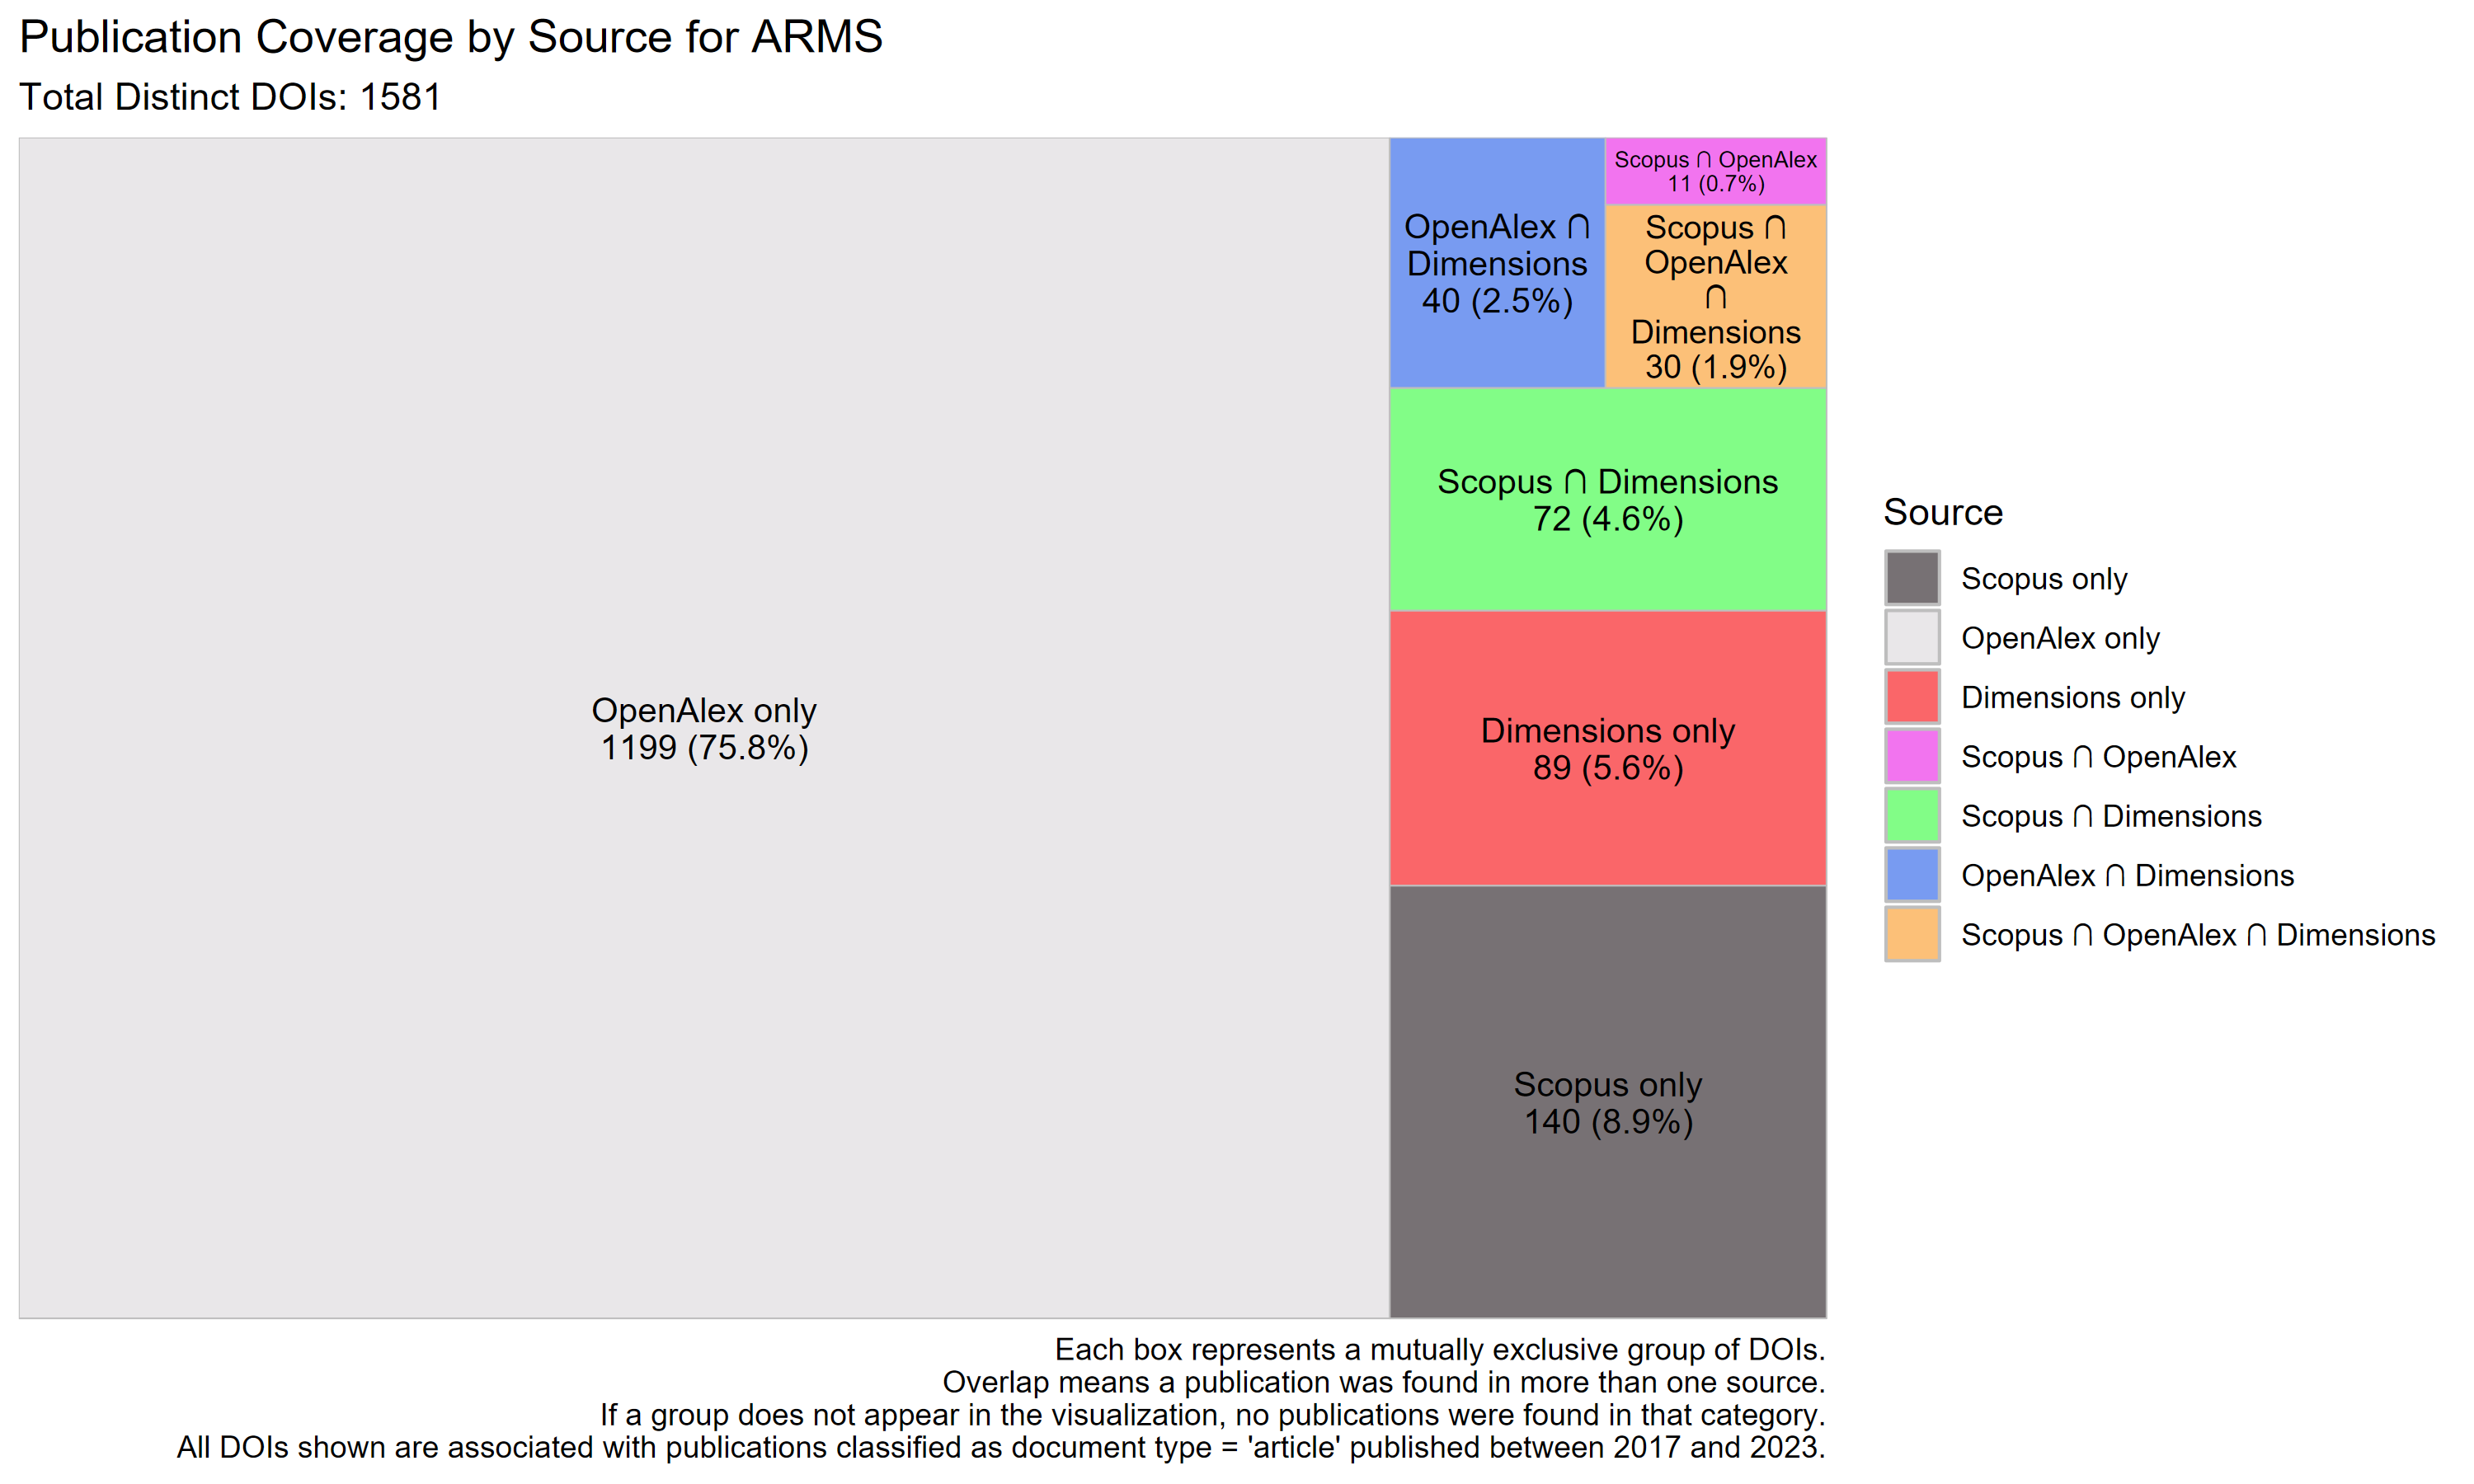
\includegraphics[keepaspectratio]{graphics/treemaps/ARMS_treemap.png}}

\paragraph*{The Census of Agriculture}\label{the-census-of-agriculture}
\addcontentsline{toc}{paragraph}{The Census of Agriculture}

Scopus provides the broadest exclusive coverage for the Census of
Agriculture, accounting for 41.3\% of DOIs. Dimensions follows at
18.8\%, while OpenAlex accounts for just 9.2\% exclusively. The largest
overlap is between Scopus and Dimensions (22.8\%), with limited
three-way overlap (3.6\%). These results indicate that Scopus and
Dimensions are the primary sources capturing publications referencing
this dataset.

\pandocbounded{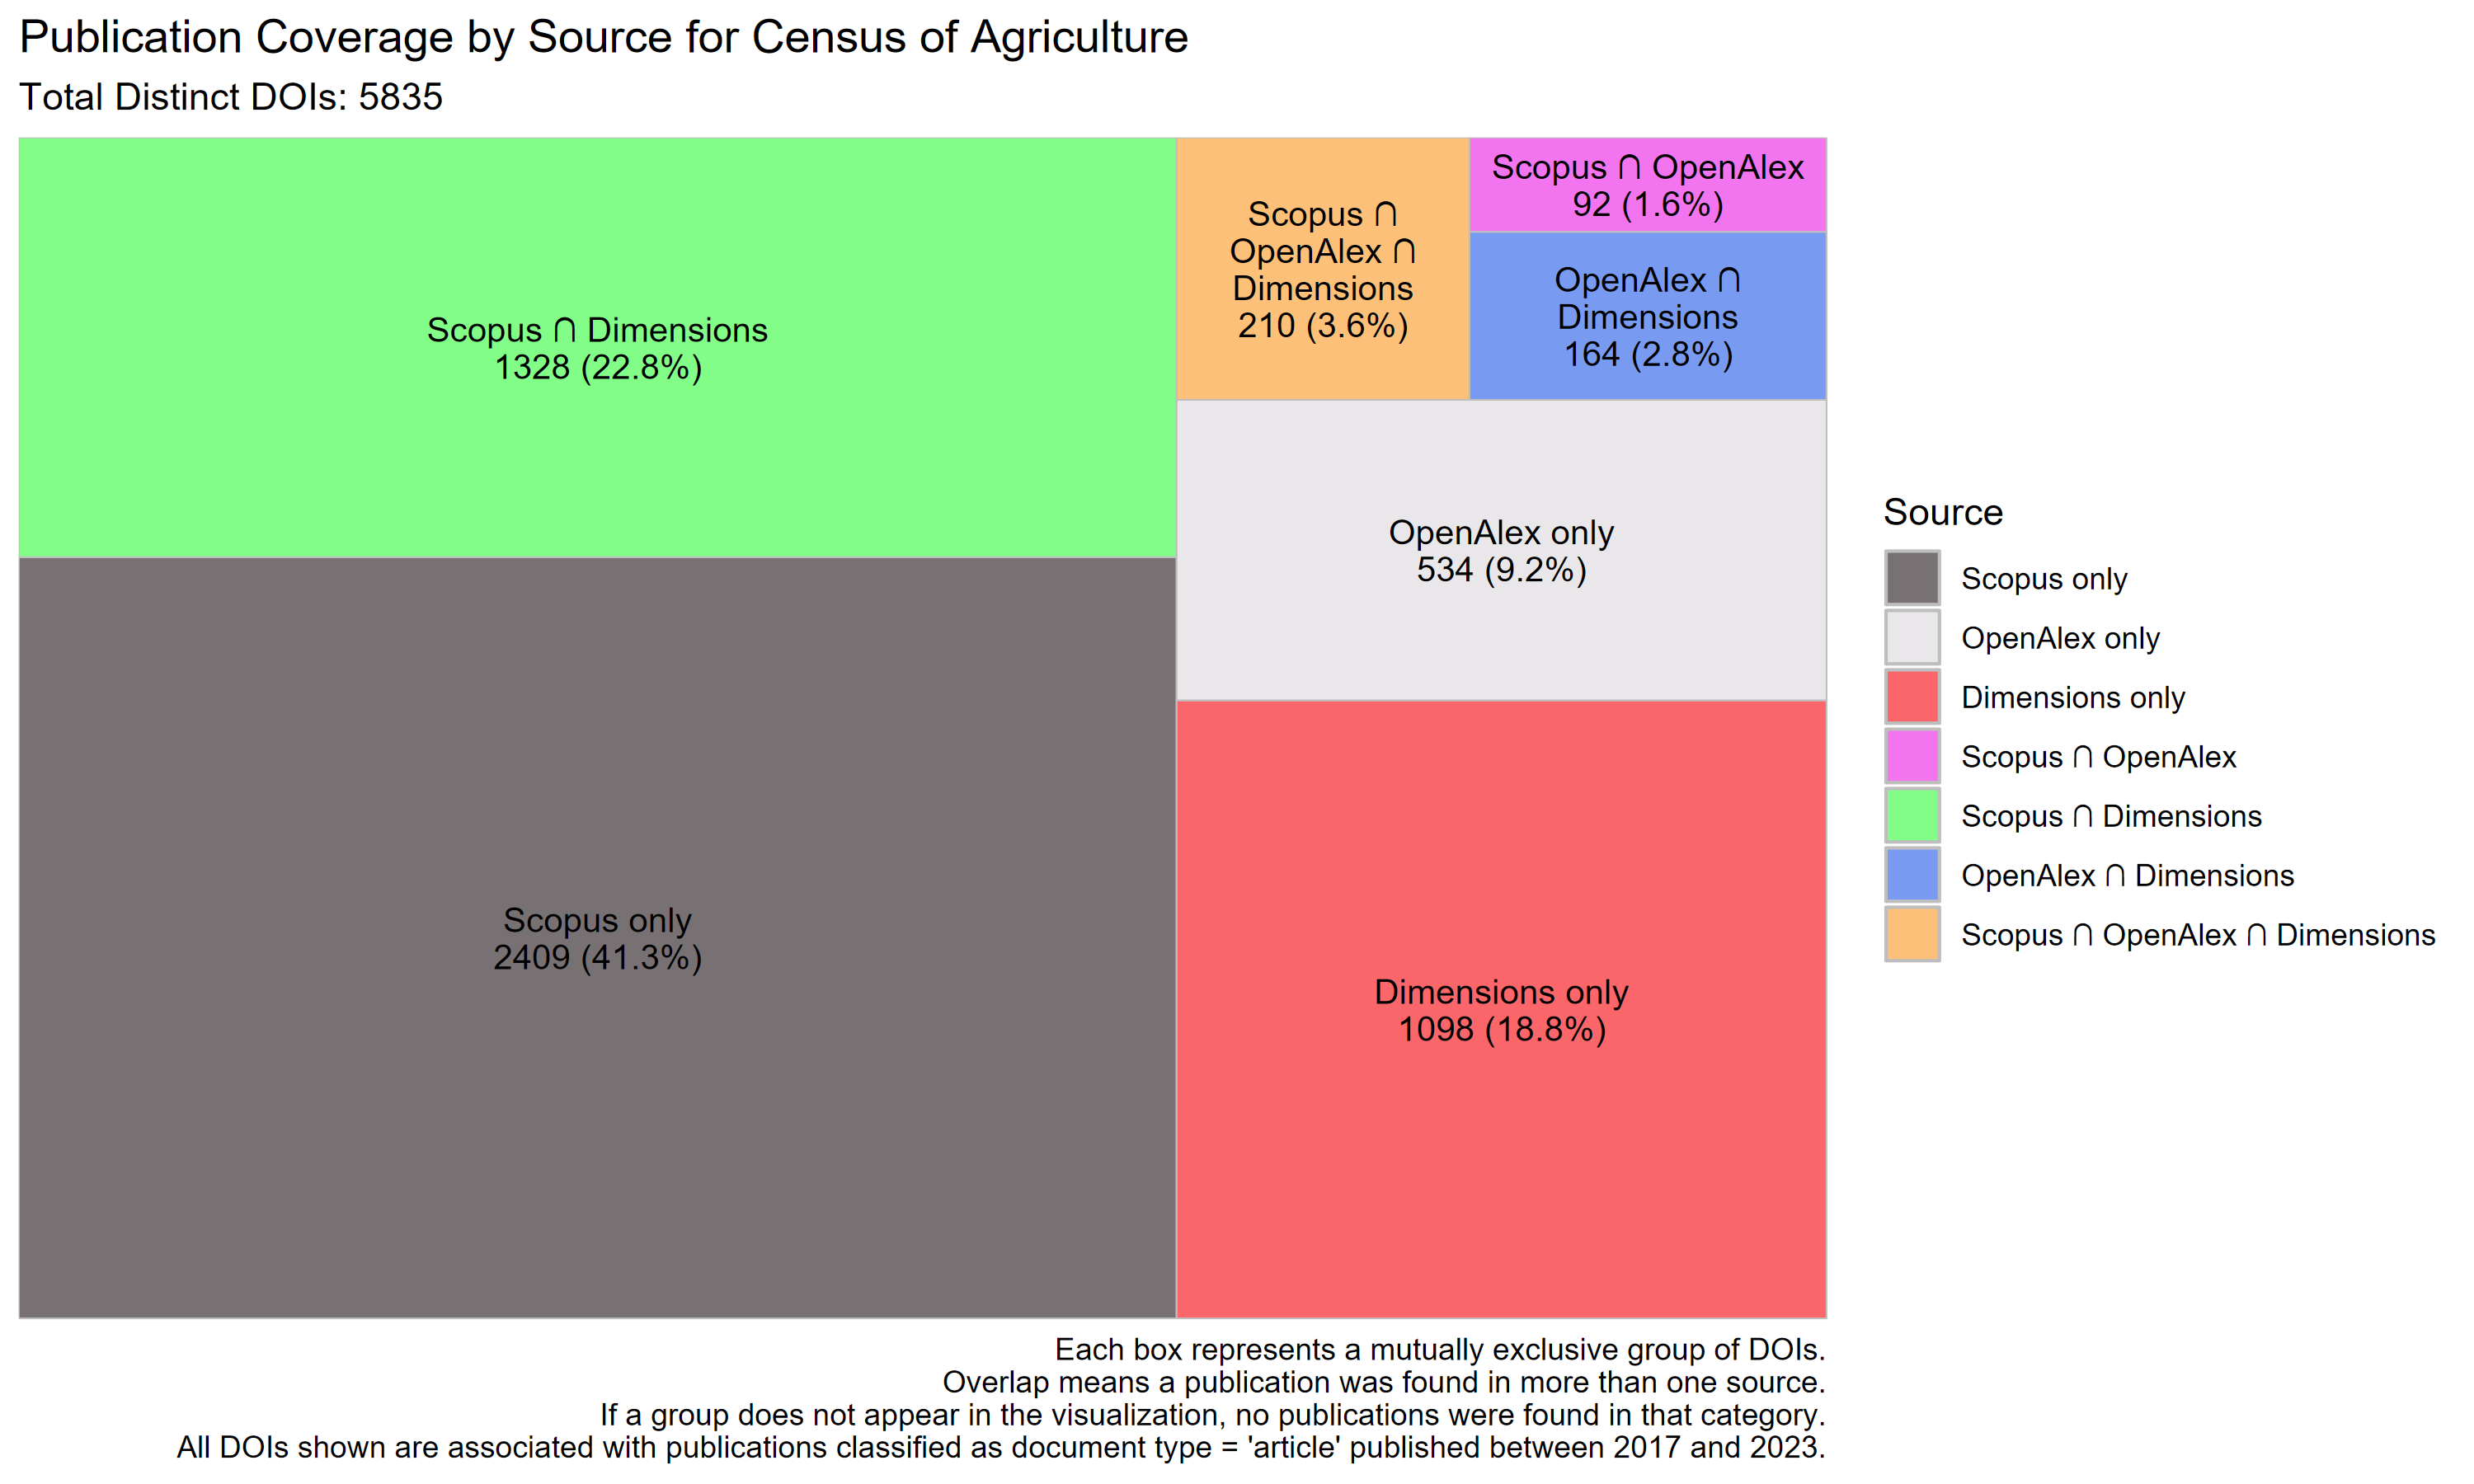
\includegraphics[keepaspectratio]{graphics/treemaps/Census_of_Agriculture_treemap.png}}

\paragraph*{Food Access Research
Atlas}\label{food-access-research-atlas}
\addcontentsline{toc}{paragraph}{Food Access Research Atlas}

Coverage for this dataset is more evenly distributed. Scopus and Scopus
∩ Dimensions each account for about 24\%, while OpenAlex-only coverage
is 14.6\%, and Dimensions-only is 11.9\%. Notably, 11\% of DOIs appear
in all three sources. This more balanced distribution suggests broader
and more consistent indexing across platforms, without a single source
dominating.

\pandocbounded{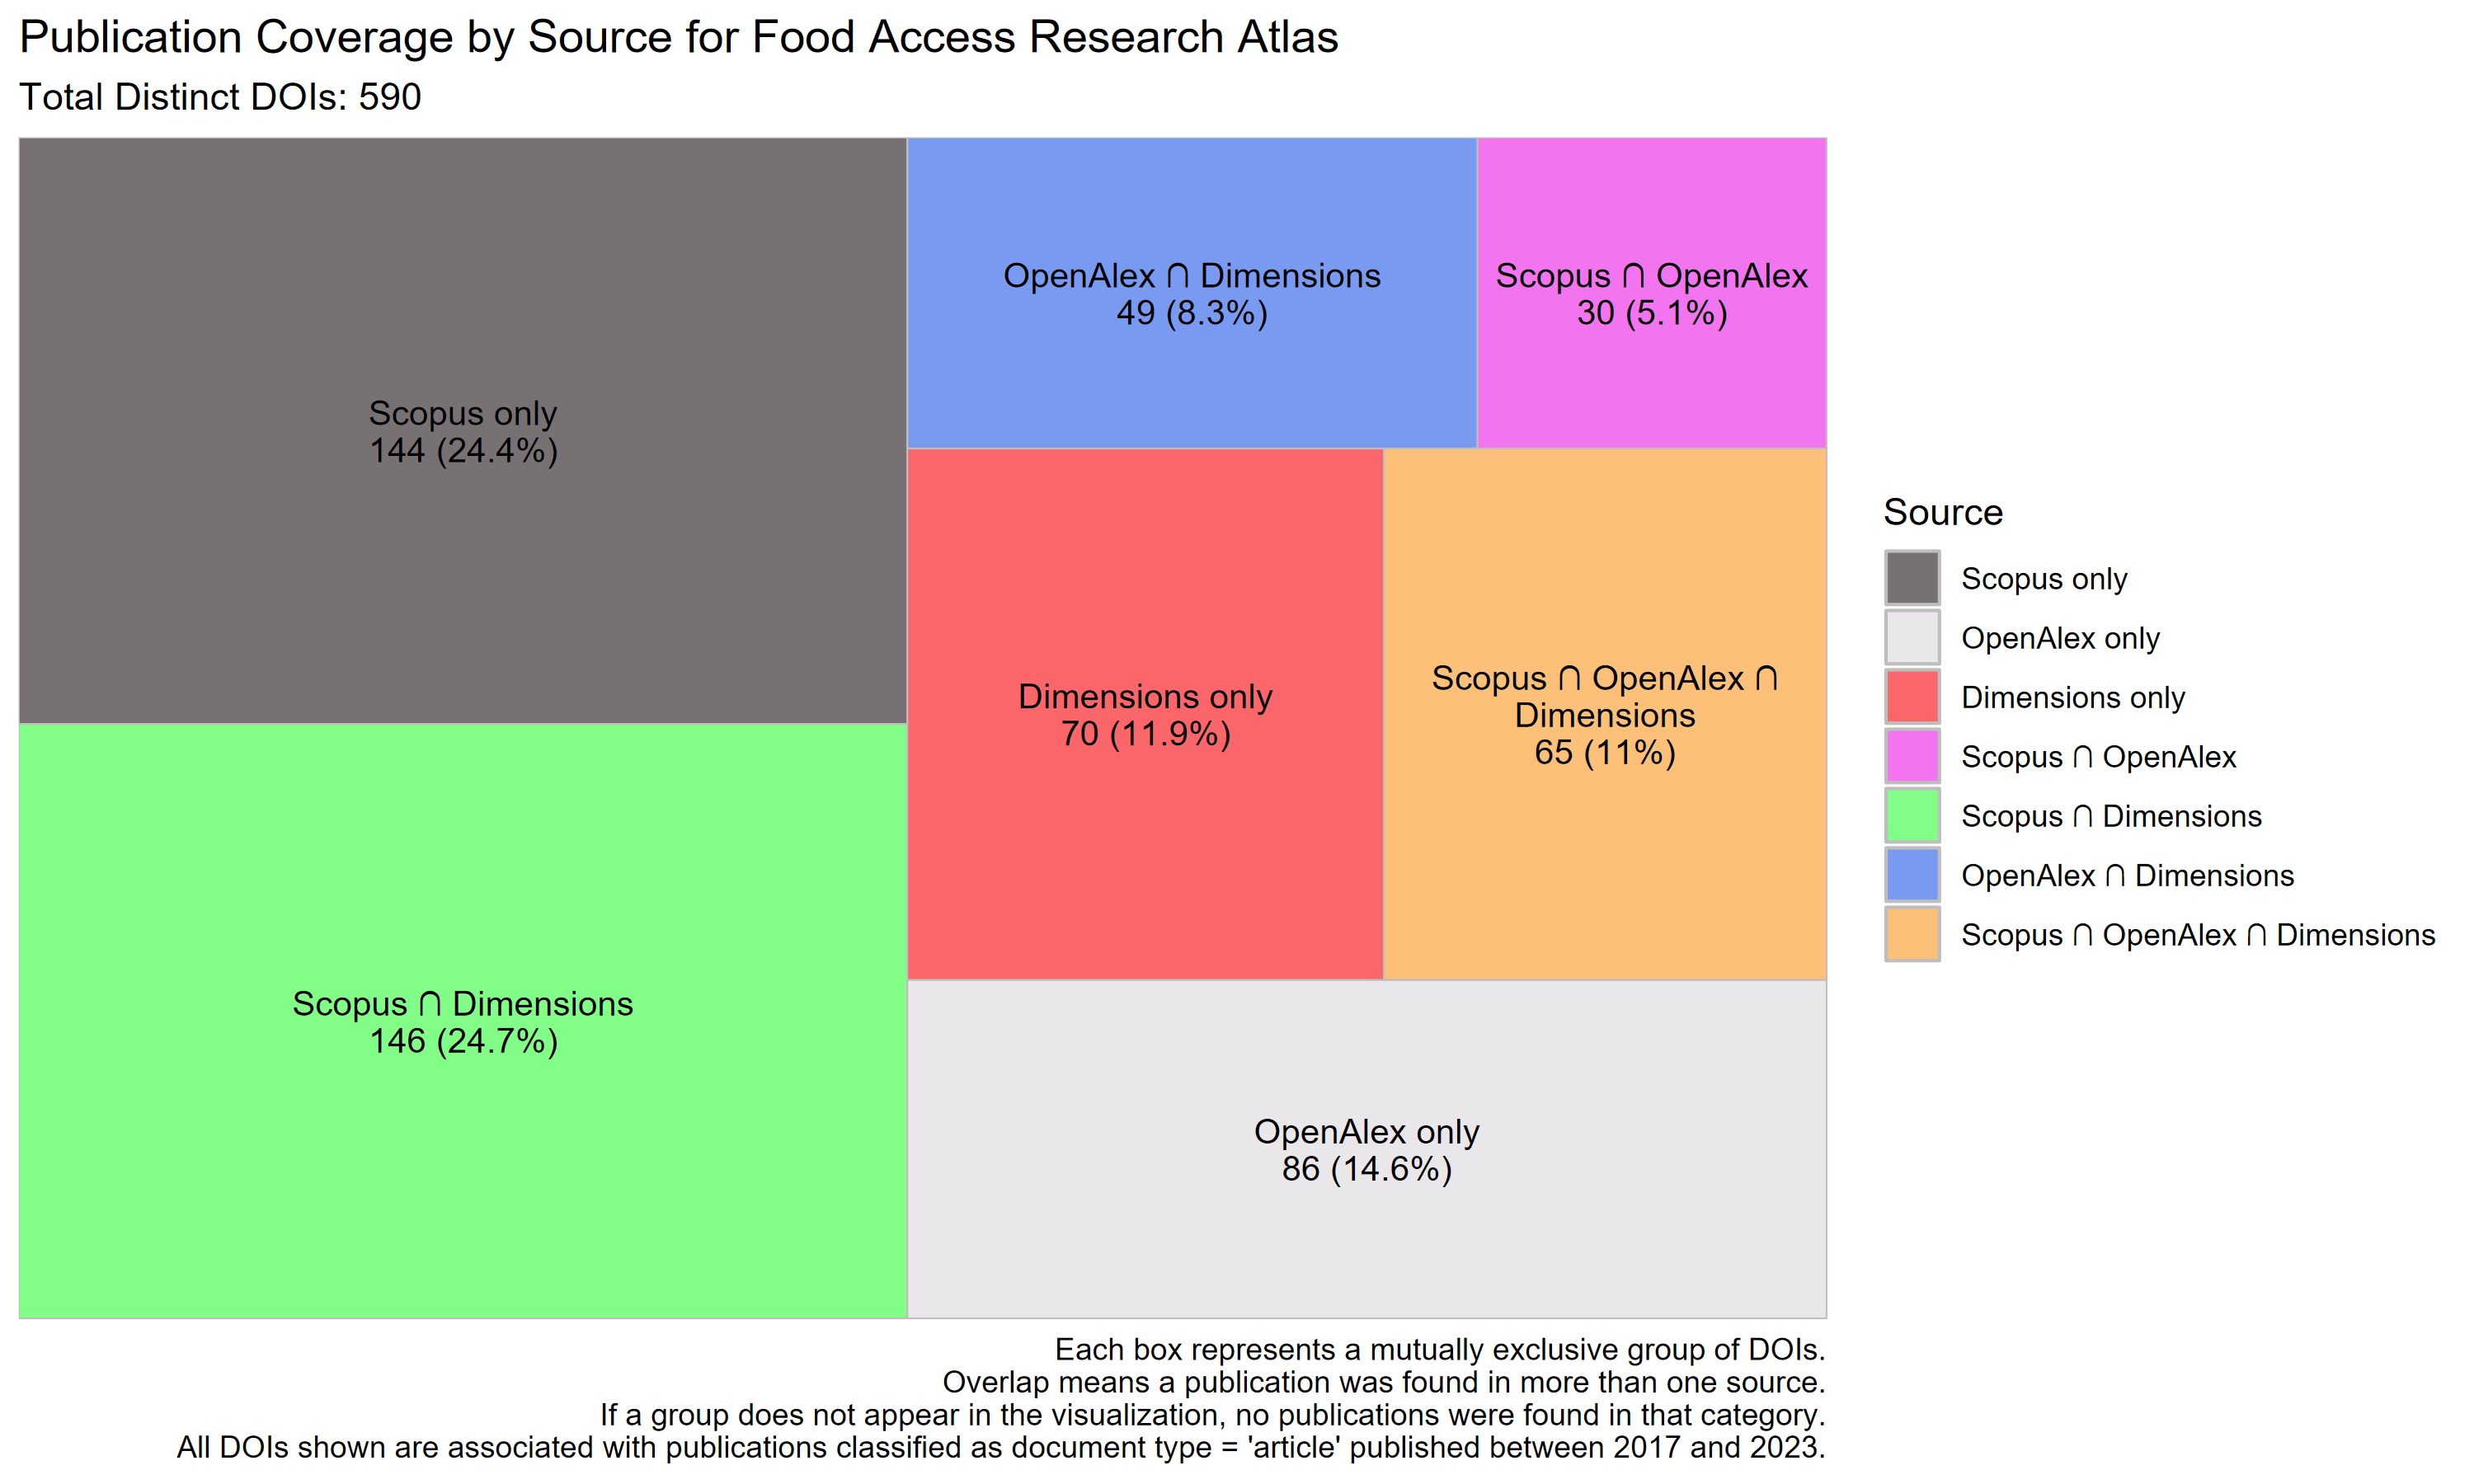
\includegraphics[keepaspectratio]{graphics/treemaps/Food_Access_Research_Atlas_treemap.png}}

\paragraph*{The Food Acquisition and Purchase Survey
(FoodAPS)}\label{the-food-acquisition-and-purchase-survey-foodaps}
\addcontentsline{toc}{paragraph}{The Food Acquisition and Purchase
Survey (FoodAPS)}

OpenAlex again provides the widest exclusive coverage (46.7\%), while
Scopus and Scopus ∩ Dimensions each contribute 17.8\%. Dimensions-only
coverage is modest (7.7\%), and 4.7\% of DOIs are shared across all
three. This indicates that OpenAlex is especially important for
capturing FoodAPS-related work, but combined use of all three sources
increases overall visibility.

\pandocbounded{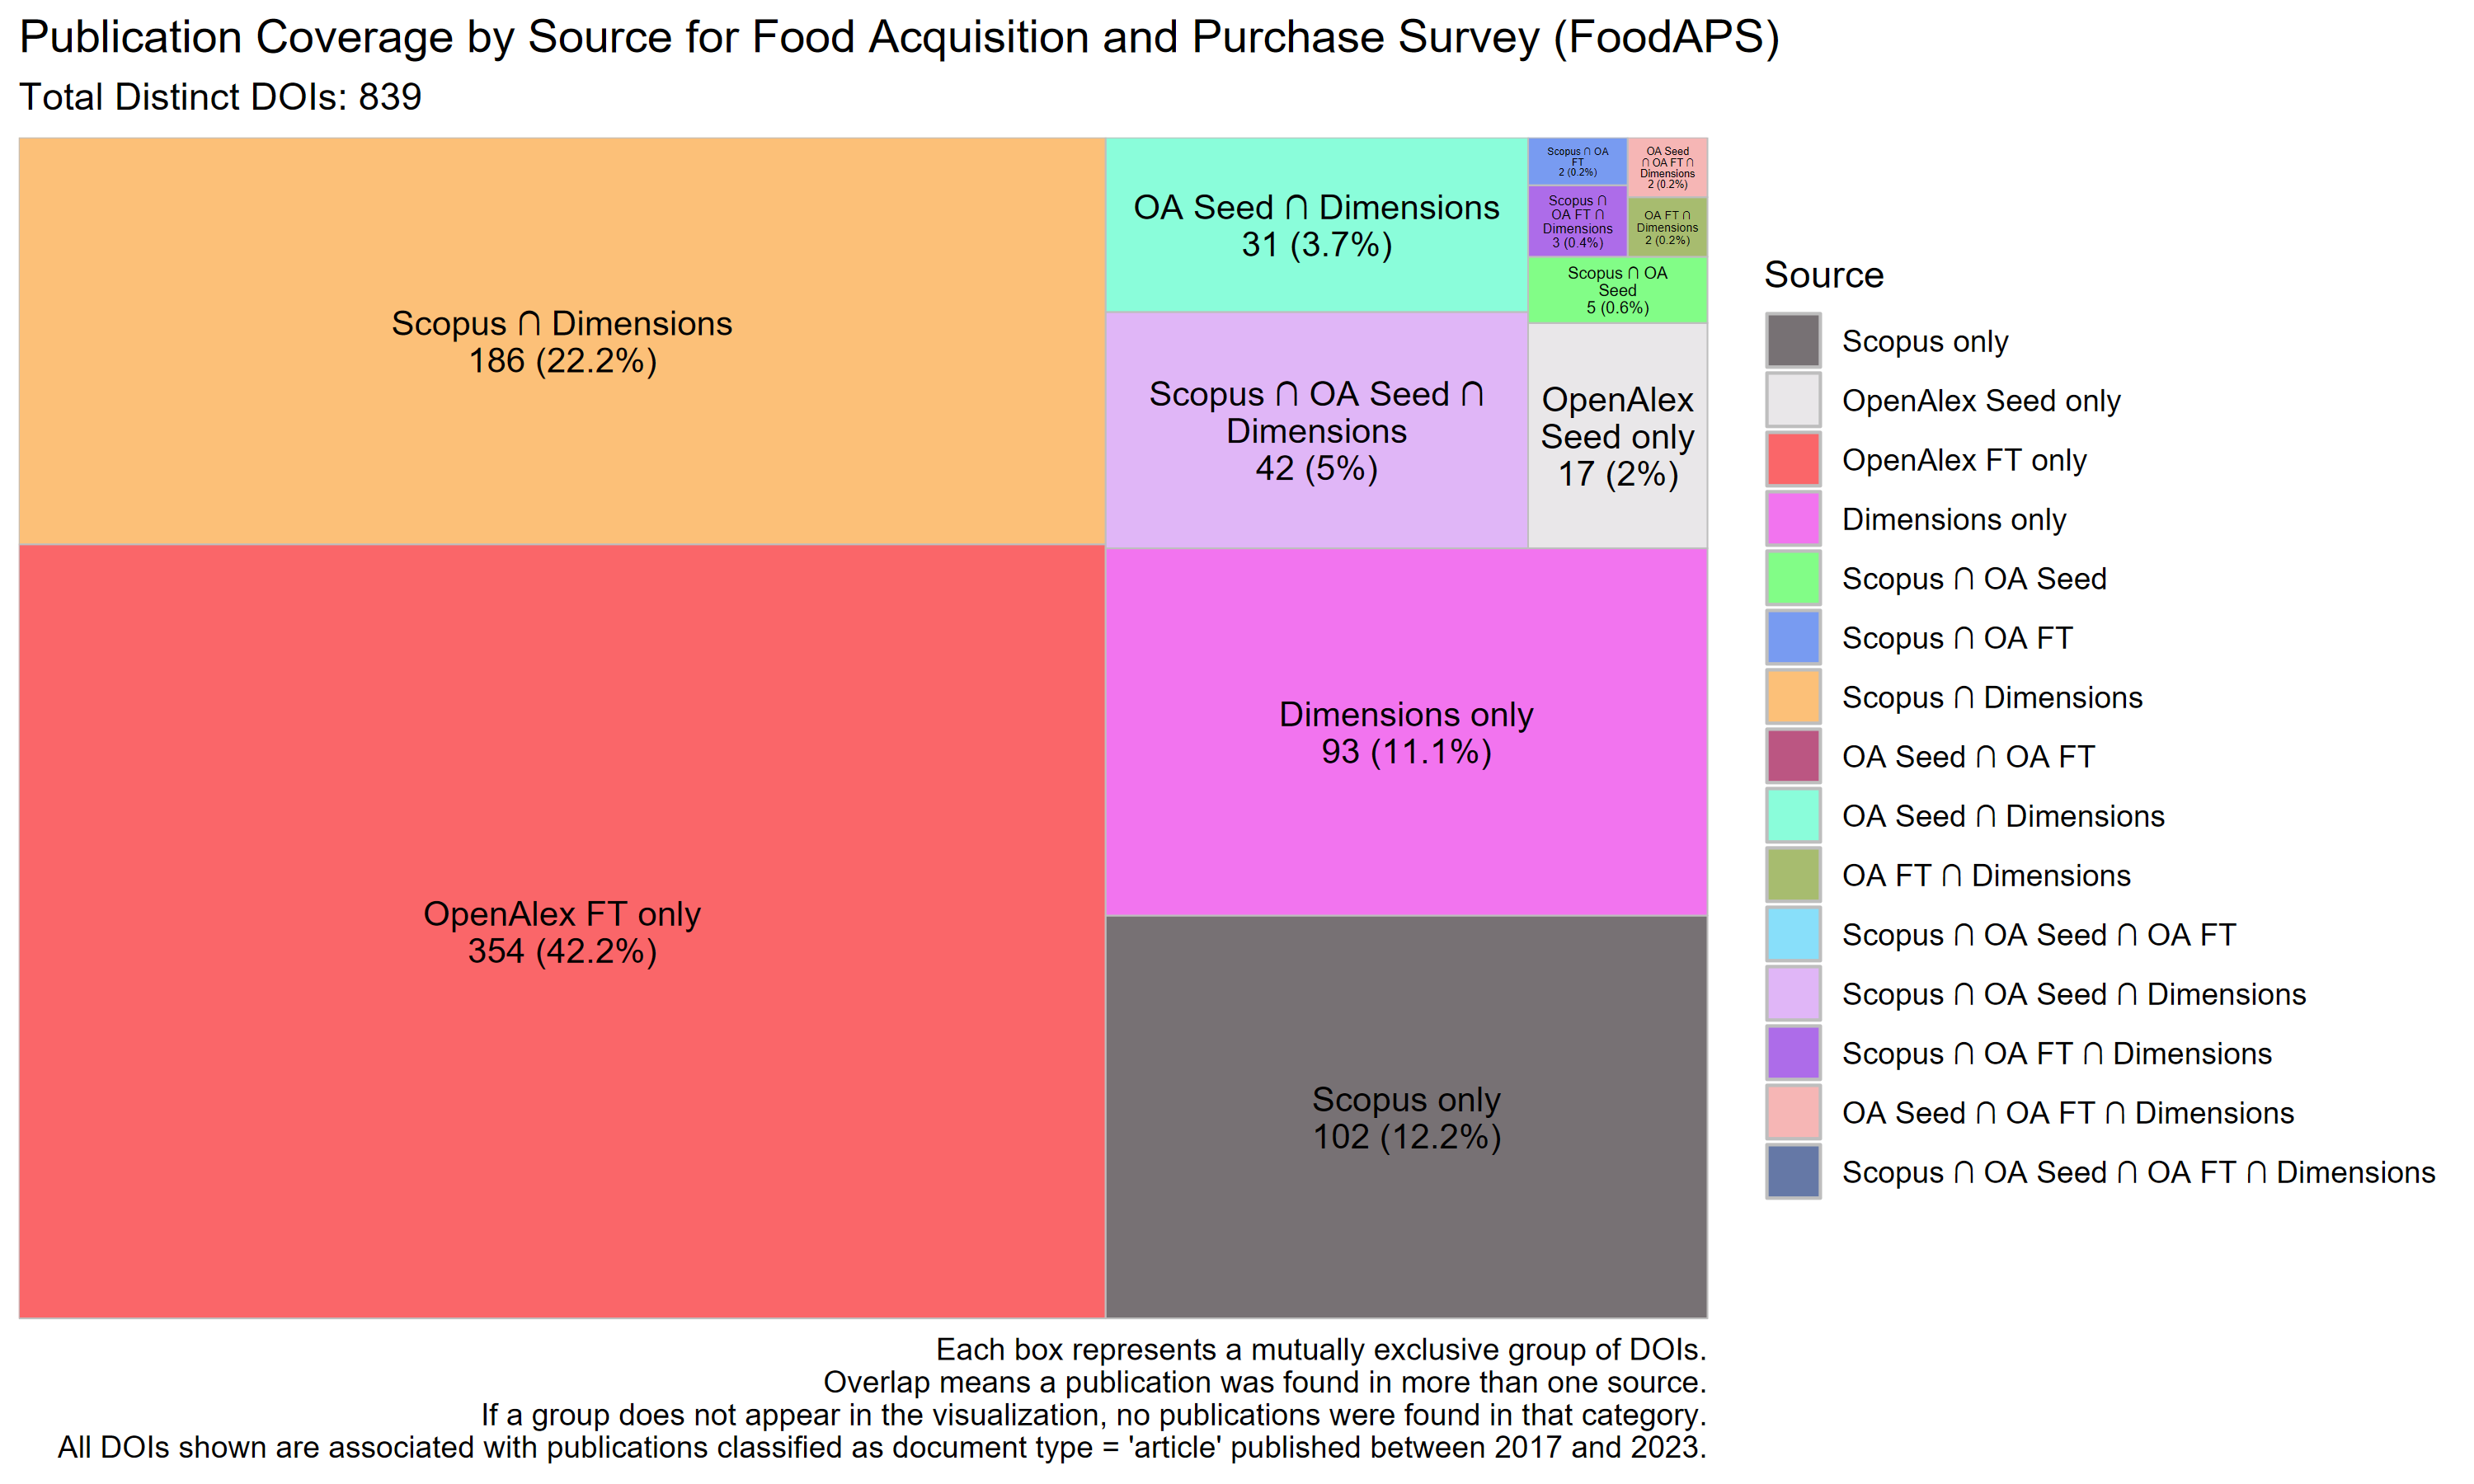
\includegraphics[keepaspectratio]{graphics/treemaps/Food_Acquisition_and_Purchase_Survey_(FoodAPS)_treemap.png}}

\paragraph*{The Household Food Security Survey
Module}\label{the-household-food-security-survey-module}
\addcontentsline{toc}{paragraph}{The Household Food Security Survey
Module}

Scopus has the highest exclusive coverage (34.7\%), followed by Scopus ∩
Dimensions (22.3\%) and Dimensions-only (17.5\%). OpenAlex-only coverage
is lower at 12.8\%, and just 5.8\% of DOIs are indexed by all three.
This indicates stronger coverage for HFSSM-related publications in
Scopus and Dimensions compared to OpenAlex.

\pandocbounded{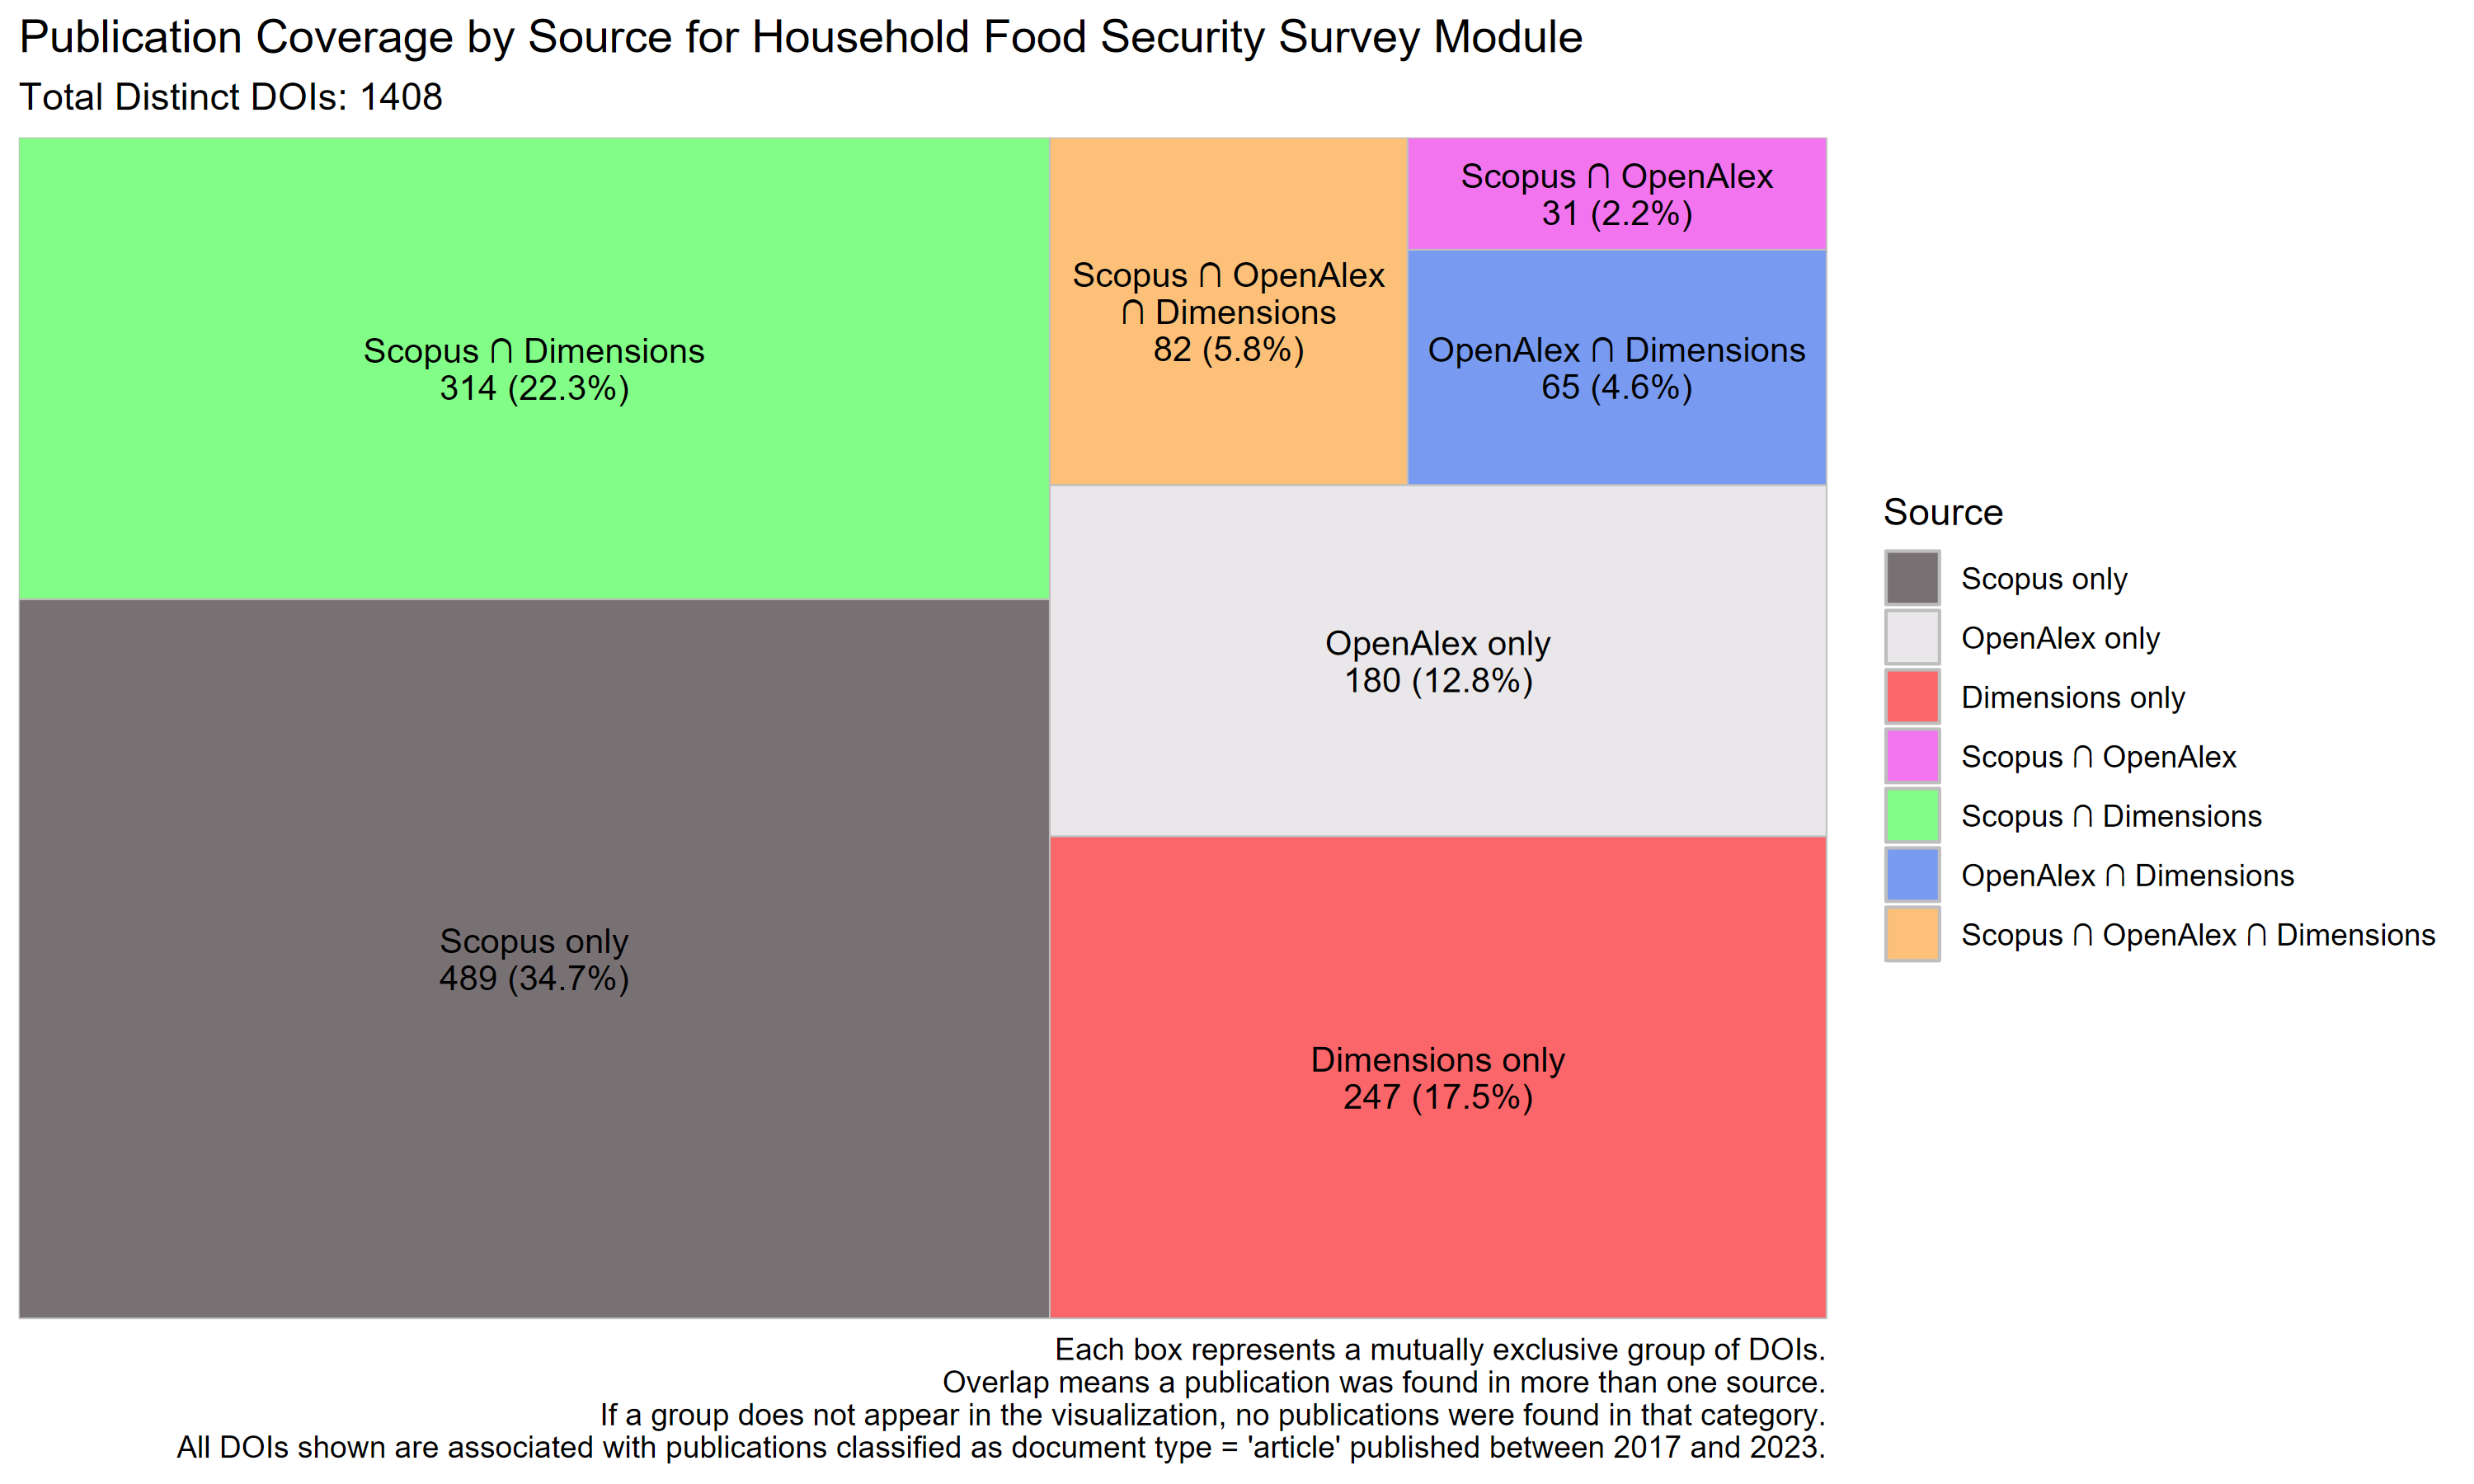
\includegraphics[keepaspectratio]{graphics/treemaps/Household_Food_Security_Survey_Module_treemap.png}}

\paragraph*{Rural-Urban Continuum
Code}\label{rural-urban-continuum-code}
\addcontentsline{toc}{paragraph}{Rural-Urban Continuum Code}

Coverage is again led by Scopus (30.8\%) and Dimensions (25\%), with
Scopus ∩ Dimensions contributing another 24.2\%. OpenAlex-only coverage
is relatively low at 8.1\%, and only 5.9\% of DOIs are shared across all
three. This pattern is consistent with datasets where OpenAlex's
coverage is more limited.

\pandocbounded{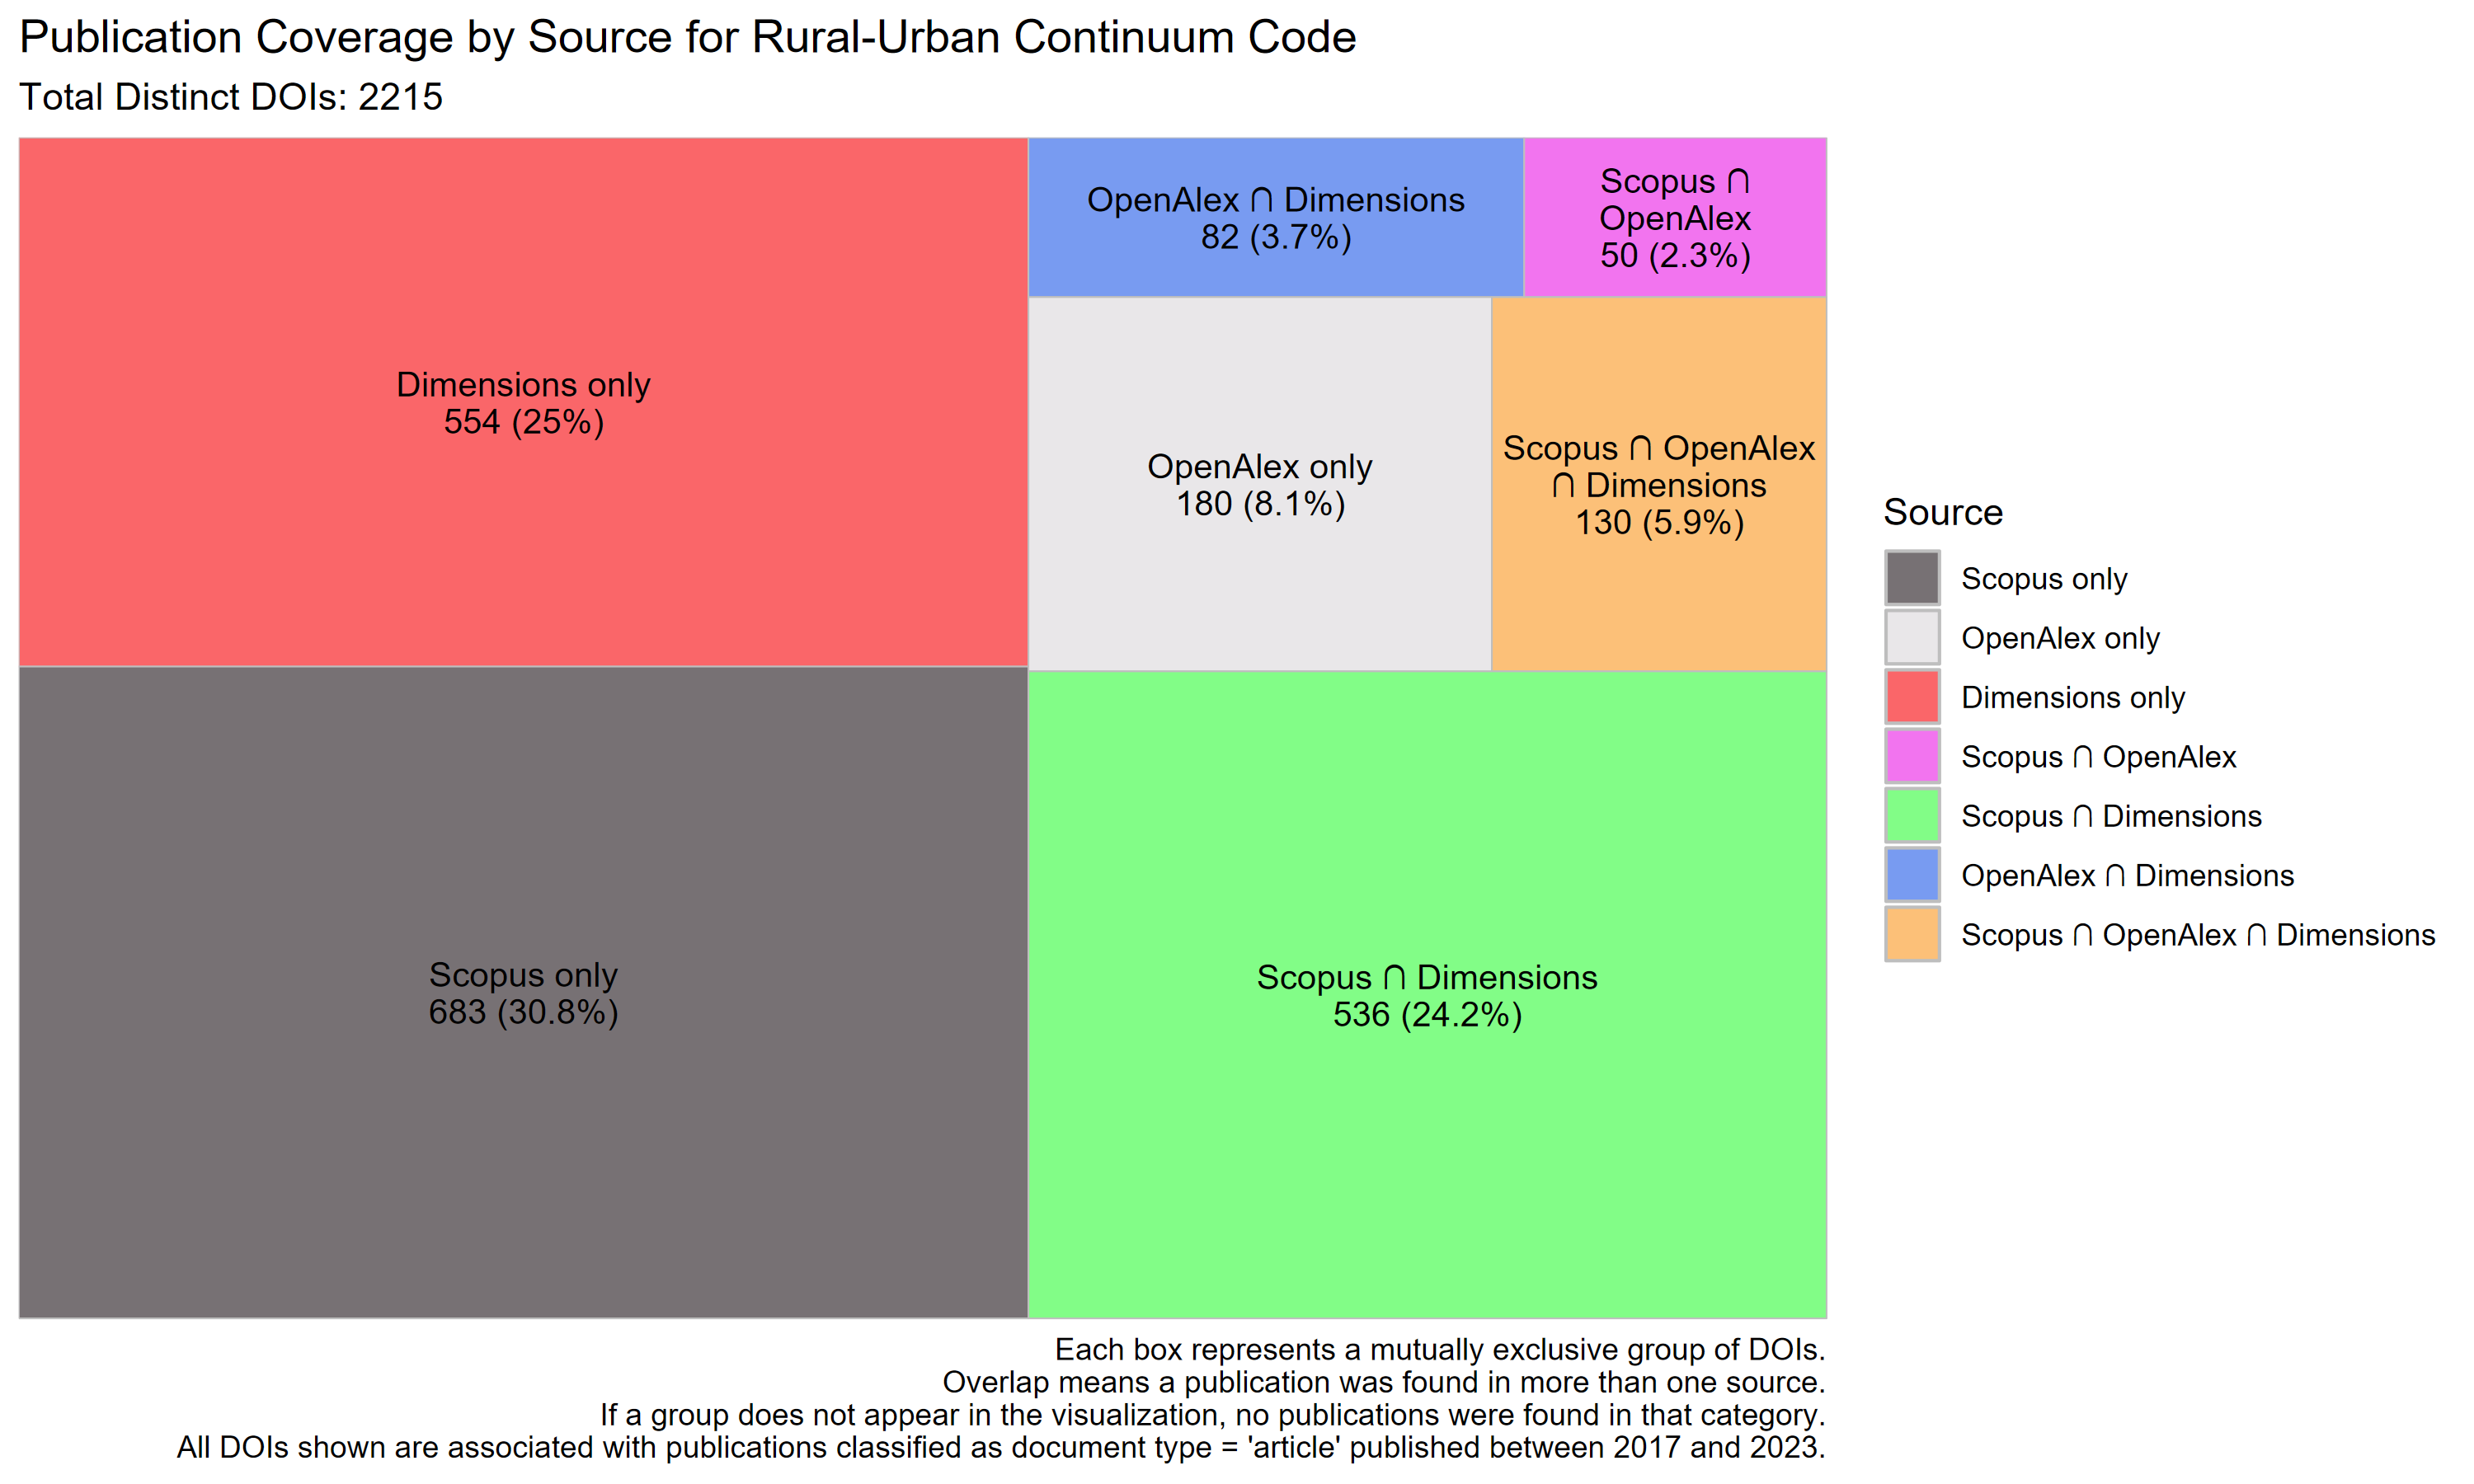
\includegraphics[keepaspectratio]{graphics/treemaps/Rural-Urban_Continuum_Code_treemap.png}}

\begin{tcolorbox}[enhanced jigsaw, leftrule=.75mm, colframe=quarto-callout-note-color-frame, toprule=.15mm, titlerule=0mm, colback=white, rightrule=.15mm, opacityback=0, breakable, bottomtitle=1mm, coltitle=black, colbacktitle=quarto-callout-note-color!10!white, left=2mm, toptitle=1mm, opacitybacktitle=0.6, title=\textcolor{quarto-callout-note-color}{\faInfo}\hspace{0.5em}{Synthesis of DOI Coverage by Source (Percent of Total DOIs)}, arc=.35mm, bottomrule=.15mm]

\begin{longtable}[]{@{}
  >{\raggedright\arraybackslash}p{(\linewidth - 16\tabcolsep) * \real{0.1436}}
  >{\raggedright\arraybackslash}p{(\linewidth - 16\tabcolsep) * \real{0.0615}}
  >{\raggedright\arraybackslash}p{(\linewidth - 16\tabcolsep) * \real{0.0923}}
  >{\raggedright\arraybackslash}p{(\linewidth - 16\tabcolsep) * \real{0.1026}}
  >{\raggedright\arraybackslash}p{(\linewidth - 16\tabcolsep) * \real{0.1128}}
  >{\raggedright\arraybackslash}p{(\linewidth - 16\tabcolsep) * \real{0.1231}}
  >{\raggedright\arraybackslash}p{(\linewidth - 16\tabcolsep) * \real{0.1333}}
  >{\raggedright\arraybackslash}p{(\linewidth - 16\tabcolsep) * \real{0.1487}}
  >{\raggedright\arraybackslash}p{(\linewidth - 16\tabcolsep) * \real{0.0821}}@{}}
\toprule\noalign{}
\begin{minipage}[b]{\linewidth}\raggedright
Dataset
\end{minipage} & \begin{minipage}[b]{\linewidth}\raggedright
Total DOIs
\end{minipage} & \begin{minipage}[b]{\linewidth}\raggedright
Scopus only (\%)
\end{minipage} & \begin{minipage}[b]{\linewidth}\raggedright
OpenAlex only (\%)
\end{minipage} & \begin{minipage}[b]{\linewidth}\raggedright
Dimensions only (\%)
\end{minipage} & \begin{minipage}[b]{\linewidth}\raggedright
Scopus ∩ OpenAlex (\%)
\end{minipage} & \begin{minipage}[b]{\linewidth}\raggedright
Scopus ∩ Dimensions (\%)
\end{minipage} & \begin{minipage}[b]{\linewidth}\raggedright
OpenAlex ∩ Dimensions (\%)
\end{minipage} & \begin{minipage}[b]{\linewidth}\raggedright
All three (\%)
\end{minipage} \\
\midrule\noalign{}
\endhead
\bottomrule\noalign{}
\endlastfoot
ARMS & 1581 & 8.9 & 75.8 & 5.6 & 0.7 & 4.6 & 2.5 & 1.9 \\
Census of Agriculture & 5835 & 41.3 & 9.2 & 18.8 & 1.6 & 22.8 & 2.8 &
3.6 \\
Food Access Research Atlas & 590 & 24.4 & 14.6 & 11.9 & 5.1 & 24.7 & 8.3
& 11.0 \\
FoodAPS & 808 & 17.8 & 46.7 & 7.7 & 1.7 & 17.8 & 3.6 & 4.7 \\
HFSSM & 1408 & 34.7 & 12.8 & 17.5 & 2.2 & 22.3 & 4.6 & 5.8 \\
RUCC & 2215 & 30.8 & 8.1 & 25.0 & 2.3 & 24.2 & 3.7 & 5.9 \\
\end{longtable}

\end{tcolorbox}

\subsubsection{Journal Coverage}\label{journal-coverage}

The previous section documented substantial variation in publication
coverage across Scopus, OpenAlex, and Dimensions. One potential
explanation for these differences is variation in journal indexing
across sources. This section examines that possibility by looking at
journal coverage, specifically, whether each citation database indexes
the journals where USDA dataset-related publications appear.

For each dataset, the analysis identifies the top 40 journals (by DOI
count) and determines which citation databases index them. Sankey
diagrams illustrate the relationship between citation databases (left)
and journals (right). Flows indicate coverage, with journals indexed in
multiple sources connected to each. While only the top 40 journals are
visualized, a complete list is available in the
\href{https://github.com/laurenchenarides/compare_scopus_openalex_report/tree/main/graphics/sankey_plots2}{GitHub
repository}.

\paragraph*{Agricultural Resource Management Survey
(ARMS)}\label{agricultural-resource-management-survey-arms-1}
\addcontentsline{toc}{paragraph}{Agricultural Resource Management Survey
(ARMS)}

Most top journals referencing ARMS are indexed by OpenAlex, including
several high-DOI outlets such as \emph{Applied Economic Perspectives and
Policy} and the \emph{American Journal of Agricultural Economics}. Fewer
journals are exclusive to Scopus or Dimensions. This pattern aligns with
OpenAlex's dominant coverage of ARMS publications in the previous
section.

\paragraph*{The Census of
Agriculture}\label{the-census-of-agriculture-1}
\addcontentsline{toc}{paragraph}{The Census of Agriculture}

Journal coverage for Census-related publications is distributed more
evenly across the three sources. Several journals---particularly in
environmental and remote sensing fields---are indexed only in Scopus or
Dimensions. Shared indexing is common for journals like \emph{Food
Policy} and \emph{Agricultural Systems}, helping to explain the high
level of overlap between Scopus and Dimensions.

\paragraph*{Food Access Research
Atlas}\label{food-access-research-atlas-1}
\addcontentsline{toc}{paragraph}{Food Access Research Atlas}

This dataset is associated with journals that are broadly indexed across
sources. Titles such as the \emph{Journal of Agricultural and Applied
Economics} and \emph{Ecological Economics} are covered in all three
databases. The strong overlap in journal indexing corresponds with the
relatively balanced publication coverage observed in the prior section.

\paragraph*{The Food Acquisition and Purchase Survey
(FoodAPS)}\label{the-food-acquisition-and-purchase-survey-foodaps-1}
\addcontentsline{toc}{paragraph}{The Food Acquisition and Purchase
Survey (FoodAPS)}

Many FoodAPS-related journals fall within the nutrition and behavioral
sciences domains, and several of these---such as \emph{Appetite} and
\emph{Frontiers in Nutrition}---are indexed in OpenAlex. While a subset
of journals is also covered by Scopus and Dimensions, OpenAlex appears
to index more of the high-volume titles, consistent with its higher
share of FoodAPS-related DOIs.

\paragraph*{The Household Food Security Survey
Module}\label{the-household-food-security-survey-module-1}
\addcontentsline{toc}{paragraph}{The Household Food Security Survey
Module}

This dataset draws from a wide range of journals in public health, food
policy, and applied economics. Journals such as \emph{Food Security} and
\emph{Journal of Nutrition Education and Behavior} appear in all three
sources, but some health-focused titles are only indexed in Scopus or
Dimensions. These differences likely contribute to the stronger coverage
seen in Scopus and Dimensions.

\paragraph*{Rural-Urban Continuum
Code}\label{rural-urban-continuum-code-1}
\addcontentsline{toc}{paragraph}{Rural-Urban Continuum Code}

Journals citing RUCC span health, epidemiology, and rural development.
Many are indexed in Scopus and Dimensions, including \emph{Environmental
Research}, \emph{BMC Public Health}, and \emph{Drug and Alcohol
Dependence}. OpenAlex has more limited coverage of these titles,
consistent with its lower representation of RUCC-related DOIs.

\begin{tcolorbox}[enhanced jigsaw, leftrule=.75mm, colframe=quarto-callout-note-color-frame, toprule=.15mm, titlerule=0mm, colback=white, rightrule=.15mm, opacityback=0, breakable, bottomtitle=1mm, coltitle=black, colbacktitle=quarto-callout-note-color!10!white, left=2mm, toptitle=1mm, opacitybacktitle=0.6, title=\textcolor{quarto-callout-note-color}{\faInfo}\hspace{0.5em}{Summary of Journal Coverage by Dataset}, arc=.35mm, bottomrule=.15mm]

\begin{longtable}[]{@{}
  >{\raggedright\arraybackslash}p{(\linewidth - 6\tabcolsep) * \real{0.1707}}
  >{\raggedright\arraybackslash}p{(\linewidth - 6\tabcolsep) * \real{0.1463}}
  >{\raggedright\arraybackslash}p{(\linewidth - 6\tabcolsep) * \real{0.2805}}
  >{\raggedright\arraybackslash}p{(\linewidth - 6\tabcolsep) * \real{0.4024}}@{}}
\toprule\noalign{}
\begin{minipage}[b]{\linewidth}\raggedright
Dataset
\end{minipage} & \begin{minipage}[b]{\linewidth}\raggedright
Dominant Source
\end{minipage} & \begin{minipage}[b]{\linewidth}\raggedright
Notable Journals Indexed in All Sources
\end{minipage} & \begin{minipage}[b]{\linewidth}\raggedright
Notable Journals Missing from Some Sources
\end{minipage} \\
\midrule\noalign{}
\endhead
\bottomrule\noalign{}
\endlastfoot
ARMS & OpenAlex & AJAE, AEPP, Agribusiness & Few missing; OpenAlex
covers most top journals \\
Census of Agriculture & Scopus / Dimensions & Food Policy, Agricultural
Systems & Environmental/remote sensing journals missing in OpenAlex \\
Food Access Research Atlas & Shared & JAAEA, Ecological Economics &
Broad overlap; minimal gaps \\
FoodAPS & OpenAlex & Food Security, Frontiers in Nutrition & Some
nutrition journals missing in Scopus/Dimensions \\
HFSSM & Scopus / Dimensions & JNED, Food Security & Some public health
journals missing in OpenAlex \\
RUCC & Scopus / Dimensions & Environmental Research, Food Policy &
Several epidemiology/health titles missing in OpenAlex \\
\end{longtable}

\end{tcolorbox}

\subsubsection{Publication Topics}\label{publication-topics}

In addition to differences in coverage and journal indexing, citation
databases vary in how they classify research content. Each system
applies a distinct taxonomy---often algorithmically generated---to
assign topics to publications. These systems function like thematic
filters, shaping how research is organized, discovered, and interpreted.

To understand how topic classification differs across sources, this
section compares the most frequent topics assigned to the same set of
publications by Scopus, OpenAlex, and Dimensions.

\textbf{Why Focus on Overlapping Publications?}

To ensure comparability, the analysis is restricted to DOIs that appear
in all three databases. This approach isolates differences in
classification by holding the underlying publication set constant. Any
observed variation reflects how each database labels and groups the same
publications.

\textbf{Word Cloud Construction}

For each dataset, the word clouds are based on frequency tables
constructed from topic metadata assigned by each source. Specifically:

\begin{itemize}
\tightlist
\item
  The analysis filters to DOIs indexed by all three sources
\item
  For each source, the corresponding topic classification schema is used
  to generate a count of how many DOIs are linked to each topic
\item
  The word clouds visualize the top 100 most frequent topics assigned by
  each source to those shared DOIs
\end{itemize}

Source-specific classification methods include:

\begin{itemize}
\tightlist
\item
  Scopus: Author keywords and ASJC codes
\item
  OpenAlex: Topic field from OpenAlex's hierarchical ontology
\item
  Dimensions: Concepts assigned using machine learning (per Dimensions
  API codebook)
\end{itemize}

A separate frequency table was generated for each source and dataset
combination. These topic counts form the basis of the word clouds shown
below.

\paragraph*{Agricultural Resource Management Survey
(ARMS)}\label{agricultural-resource-management-survey-arms-2}
\addcontentsline{toc}{paragraph}{Agricultural Resource Management Survey
(ARMS)}

These word clouds illustrate the most frequent research topics
associated with shared DOIs (N = 30) across Scopus, OpenAlex, and
Dimensions for the Agricultural Resource Management Survey (ARMS). While
all three sources reflect a core emphasis on agricultural production and
economics, the specific framing and vocabulary vary by platform:

Dimensions highlights terms grounded in applied research and
policy-oriented topics such as marketing channels, soil health, farm
succession, and cash transfers.

OpenAlex emphasizes conceptual and policy themes like agricultural
innovations and practices, organic food and agriculture, and economic
and environmental valuation.

Scopus features broader disciplinary categories and methodological terms
including economics and econometrics, biofuel, development food science,
and soil science.

The variation in topical emphasis reflects platform-specific differences
in indexing practices, subject classification systems, and coverage of
applied versus theoretical scholarship.

\paragraph{Scopus}

\pandocbounded{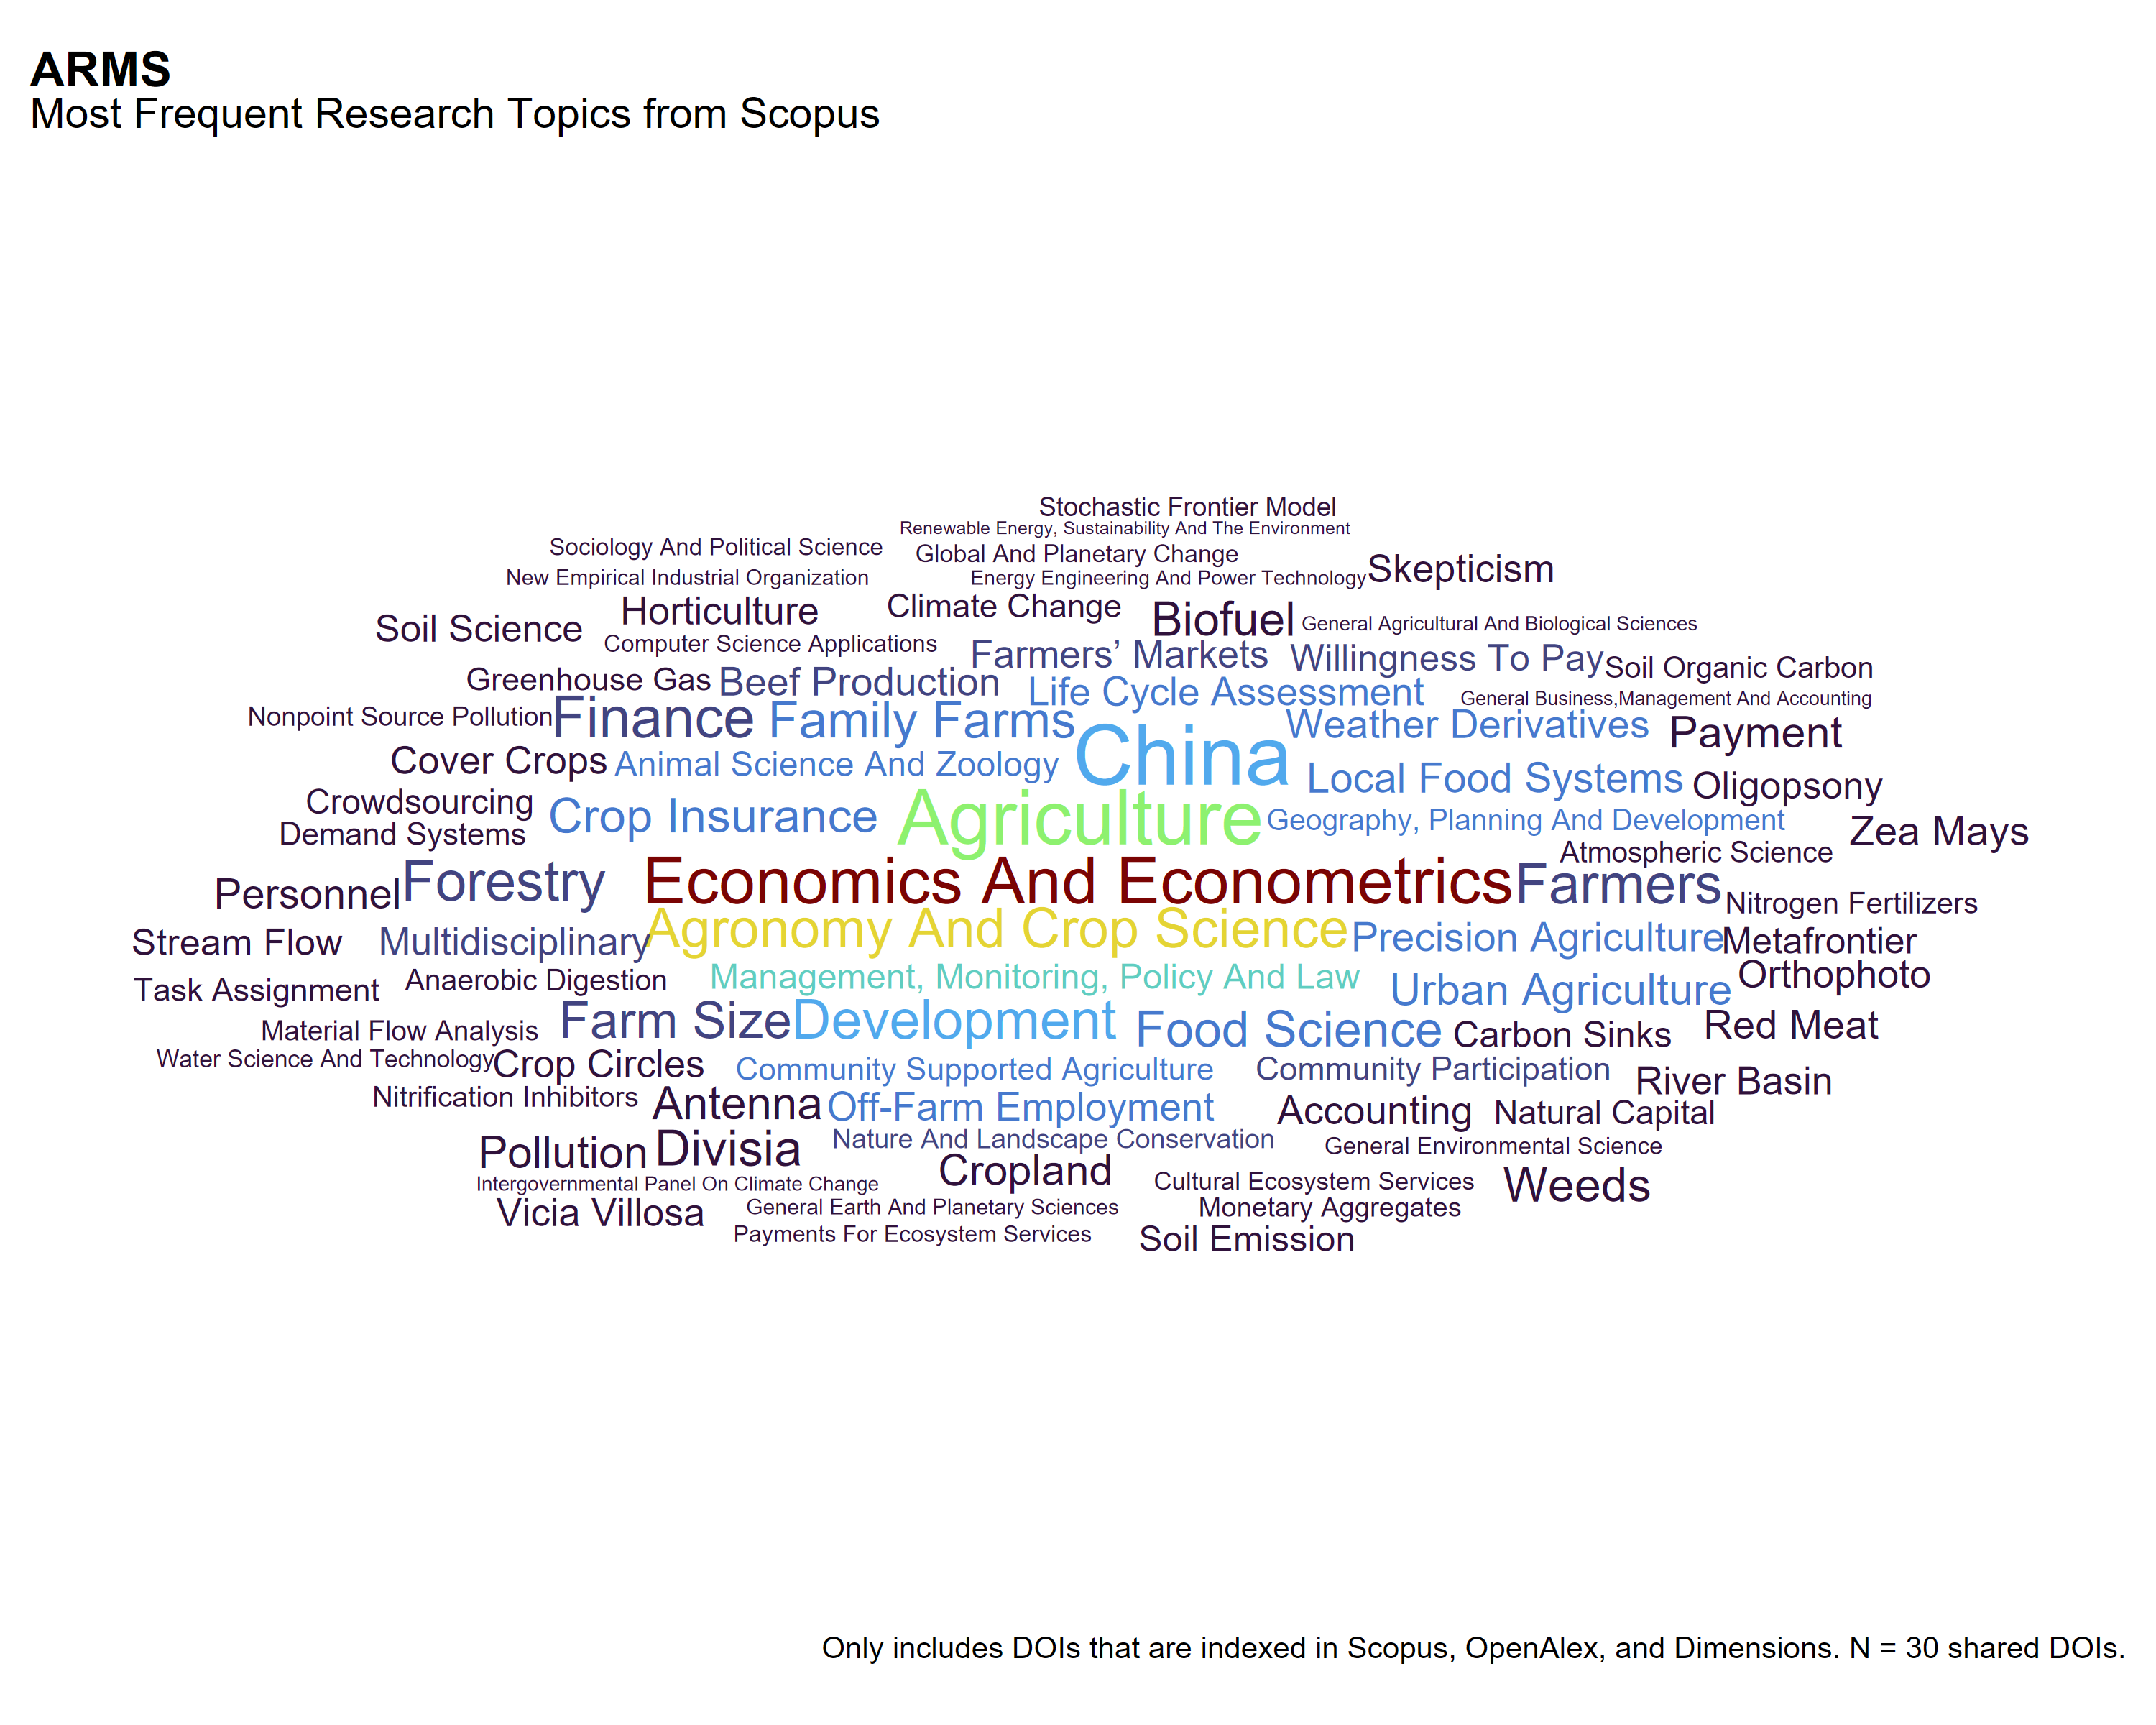
\includegraphics[keepaspectratio]{graphics/word_clouds/shared_dois/dataset01_wordcloud_shared_scopus.png}}

\paragraph{OpenAlex}

\pandocbounded{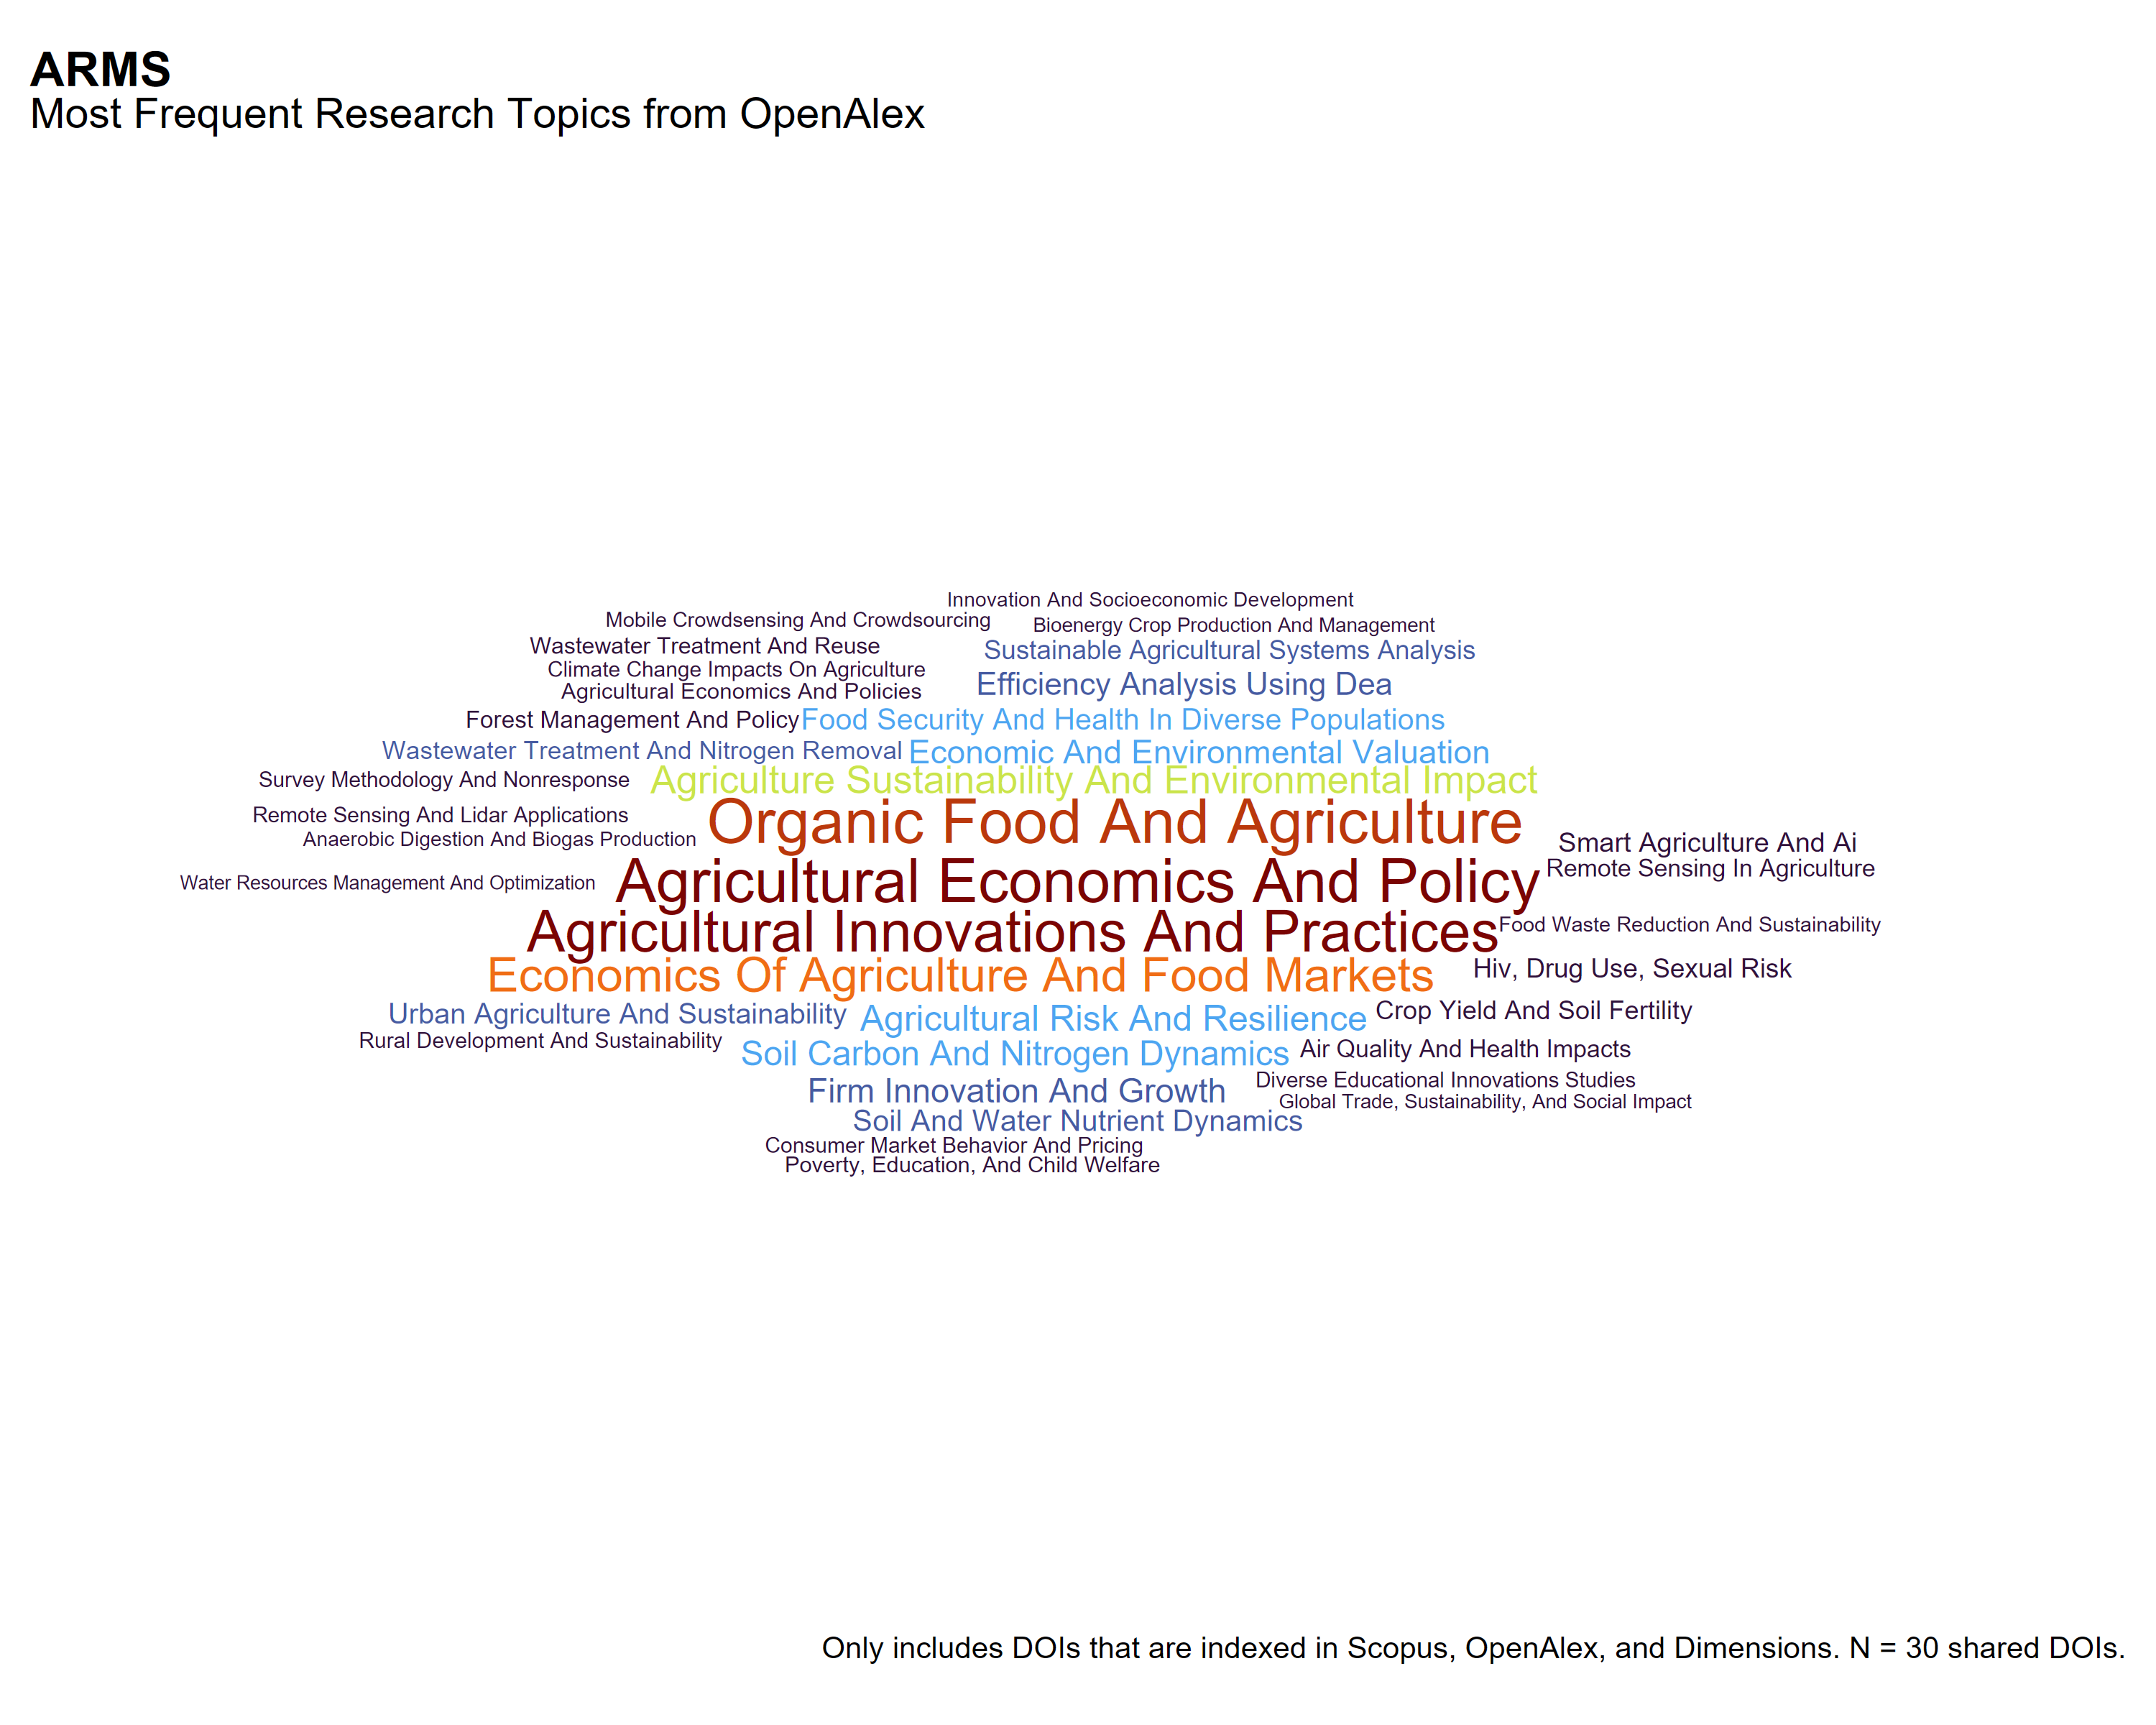
\includegraphics[keepaspectratio]{graphics/word_clouds/shared_dois/dataset01_wordcloud_shared_openalex.png}}

\paragraph{Dimensions}

\pandocbounded{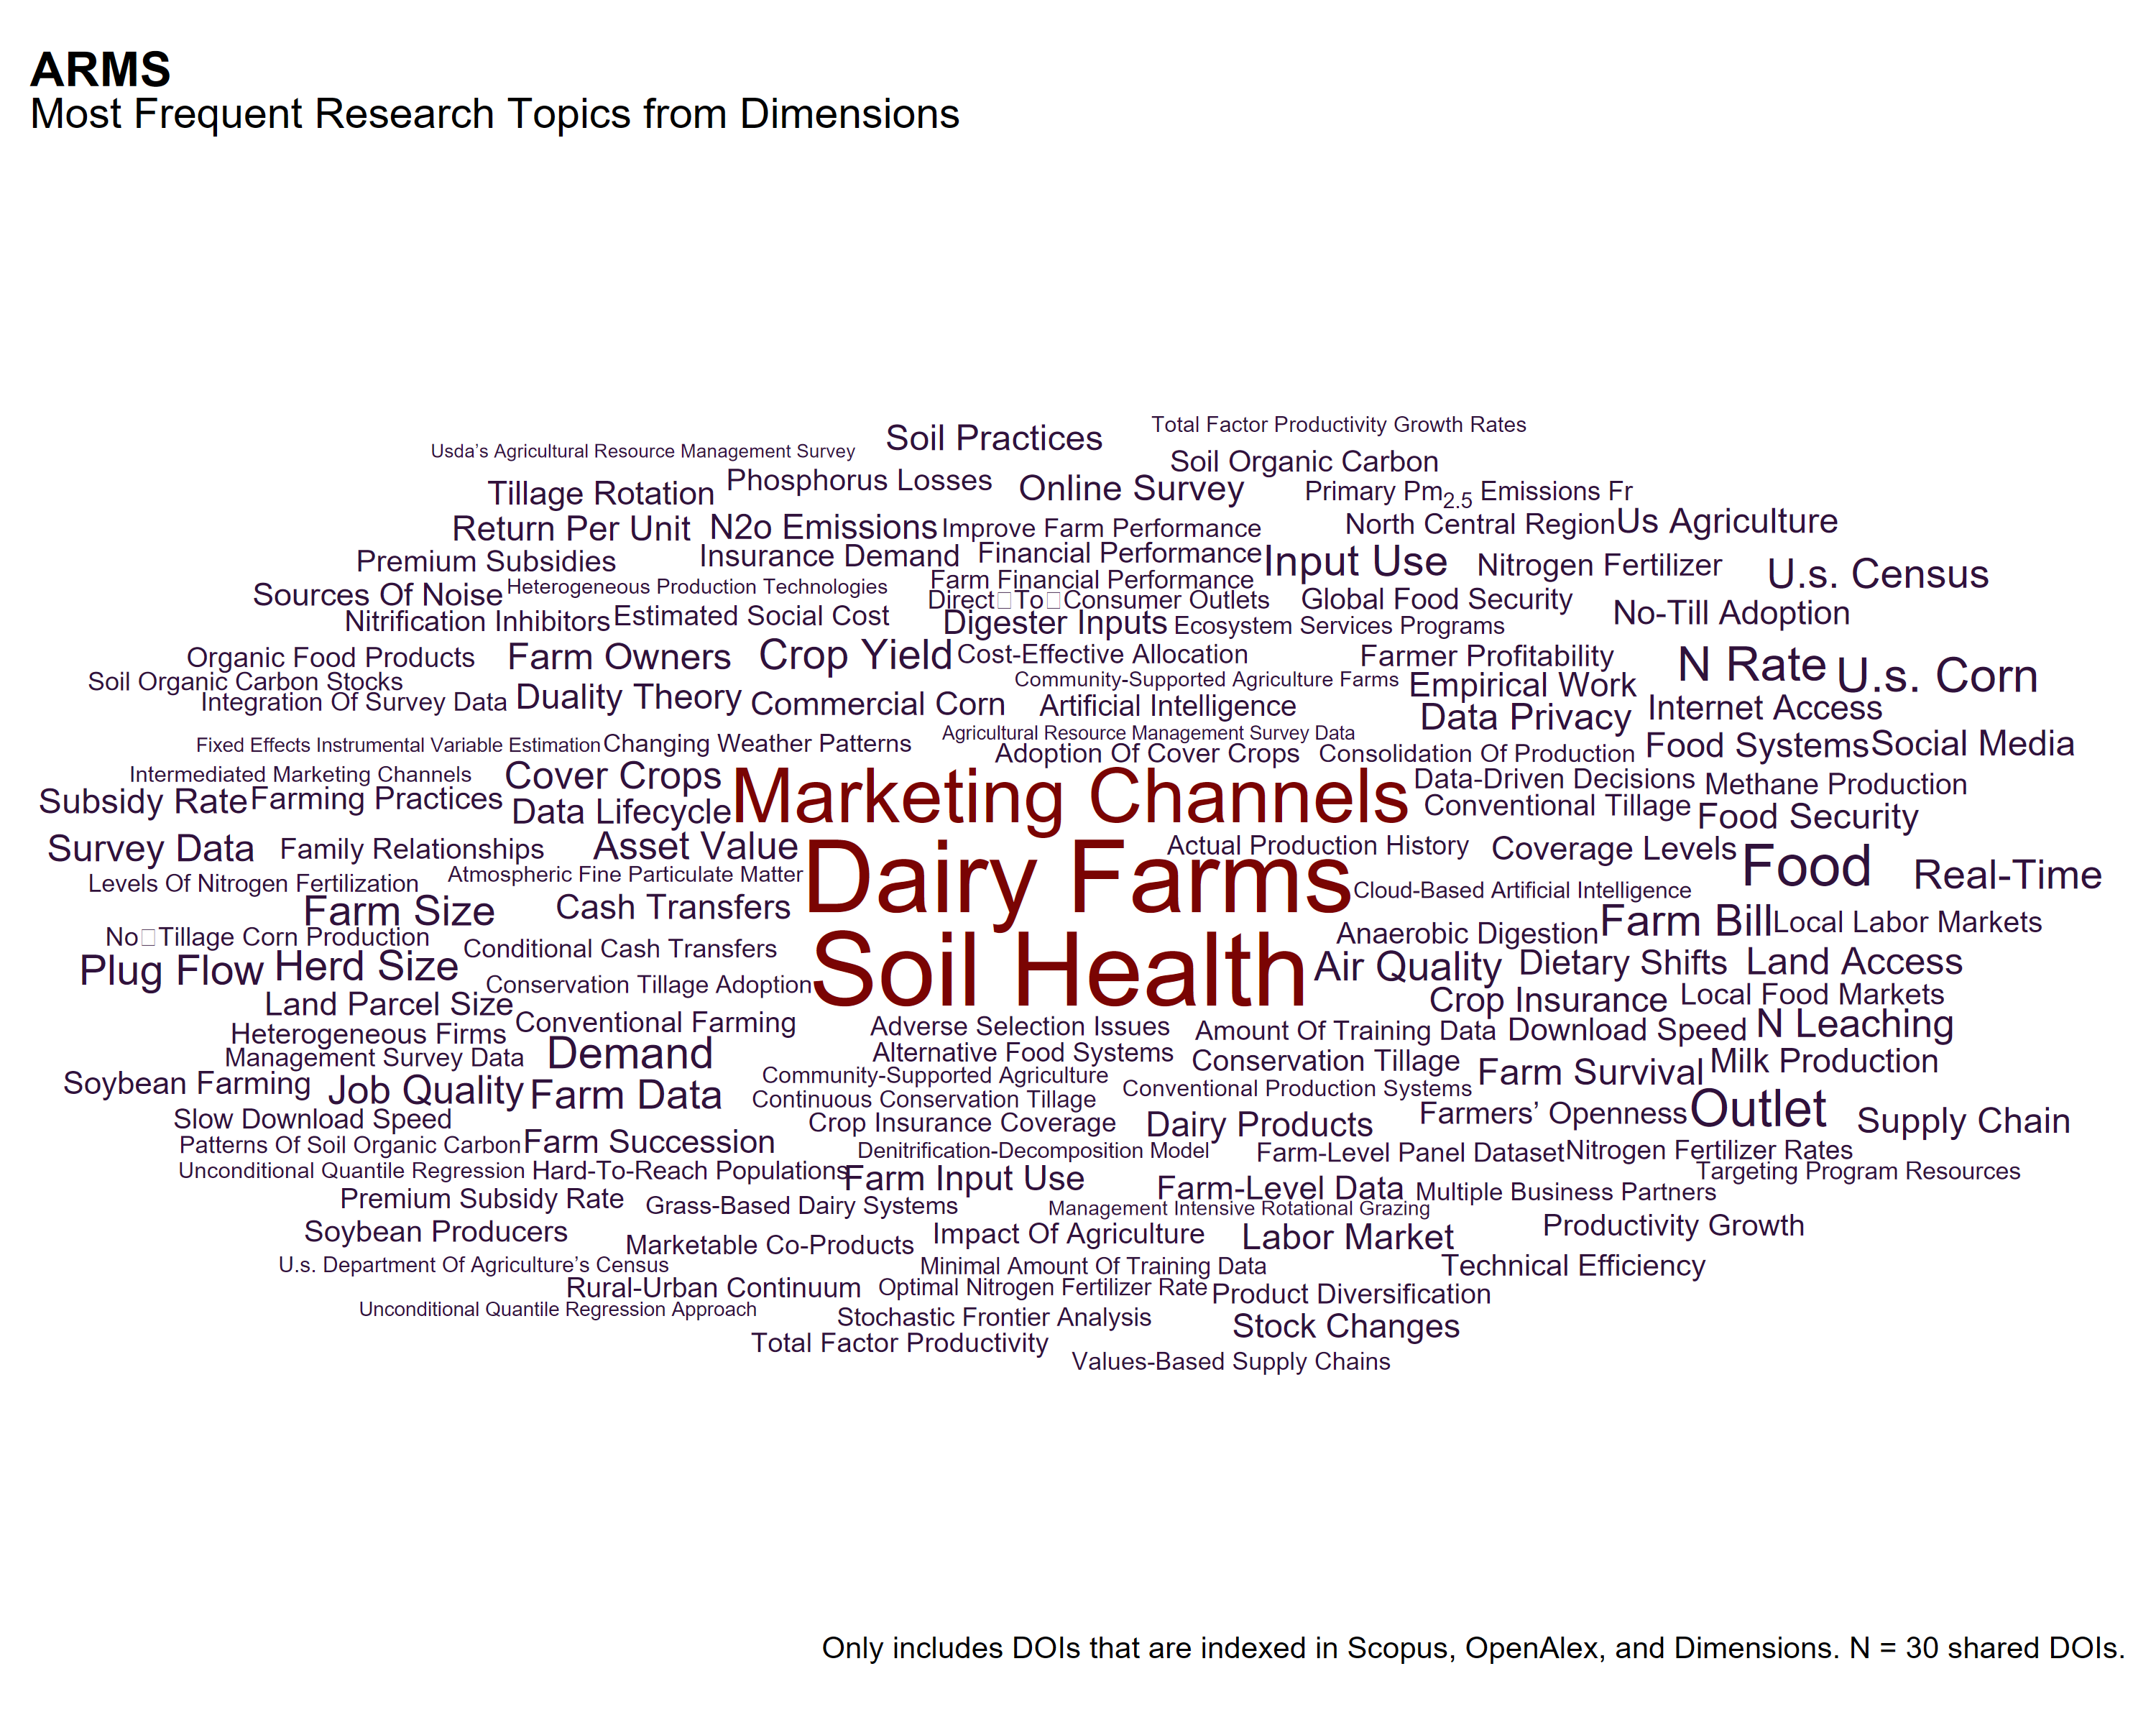
\includegraphics[keepaspectratio]{graphics/word_clouds/shared_dois/dataset01_wordcloud_shared_dimensions.png}}

The next set of word clouds summarizes the most frequent research topics
associated with publications that reference a given dataset, based on
each source's topic classification schema. The first word cloud in each
section aggregates topics across all sources---Scopus, OpenAlex, and
Dimensions---to provide a composite view of the research landscape.
Readers can then click on source-specific word clouds, which reflect the
full corpus of DOIs referencing the dataset within each source. These
differences highlight how each platform categorizes scholarly content
and may inform decisions about dataset visibility and disciplinary
reach.

\begin{tcolorbox}[enhanced jigsaw, leftrule=.75mm, colframe=quarto-callout-note-color-frame, toprule=.15mm, titlerule=0mm, colback=white, rightrule=.15mm, opacityback=0, breakable, bottomtitle=1mm, coltitle=black, colbacktitle=quarto-callout-note-color!10!white, left=2mm, toptitle=1mm, opacitybacktitle=0.6, title=\textcolor{quarto-callout-note-color}{\faInfo}\hspace{0.5em}{Additional Word Cloud Variants}, arc=.35mm, bottomrule=.15mm]

\end{tcolorbox}

\paragraph*{The Census of
Agriculture}\label{the-census-of-agriculture-2}
\addcontentsline{toc}{paragraph}{The Census of Agriculture}

The word clouds below visualize the most frequent topics assigned to the
210 publications referencing the Census of Agriculture that are indexed
in Scopus, OpenAlex, and Dimensions. The first image aggregates topic
terms across all three sources. The remaining word clouds show how each
individual source categorizes the same set of publications.

Each classification system presents a different view of the research
landscape:

Dimensions emphasizes applied agricultural practice and land management
topics, such as Cover Crops, Food Systems, Land Use, and No-Till. Many
of the terms reflect production methods, conservation, and on-farm
activities.

OpenAlex includes a wider range of thematic areas, with terms related to
sustainability, valuation, and interdisciplinary research. Examples
include Urban Agriculture and Sustainability, Economic and Environmental
Valuation, and Food Waste Reduction.

Scopus reflects more traditional disciplinary structures, with emphasis
on Ecology, Food Science, Economics and Econometrics, and Soil Emission.
The presence of terms like China and Urban Agriculture points to
geographic and policy framing as well.

These differences reflect variation in how each source structures and
assigns topical metadata to the same publications.

\paragraph{Scopus}

\pandocbounded{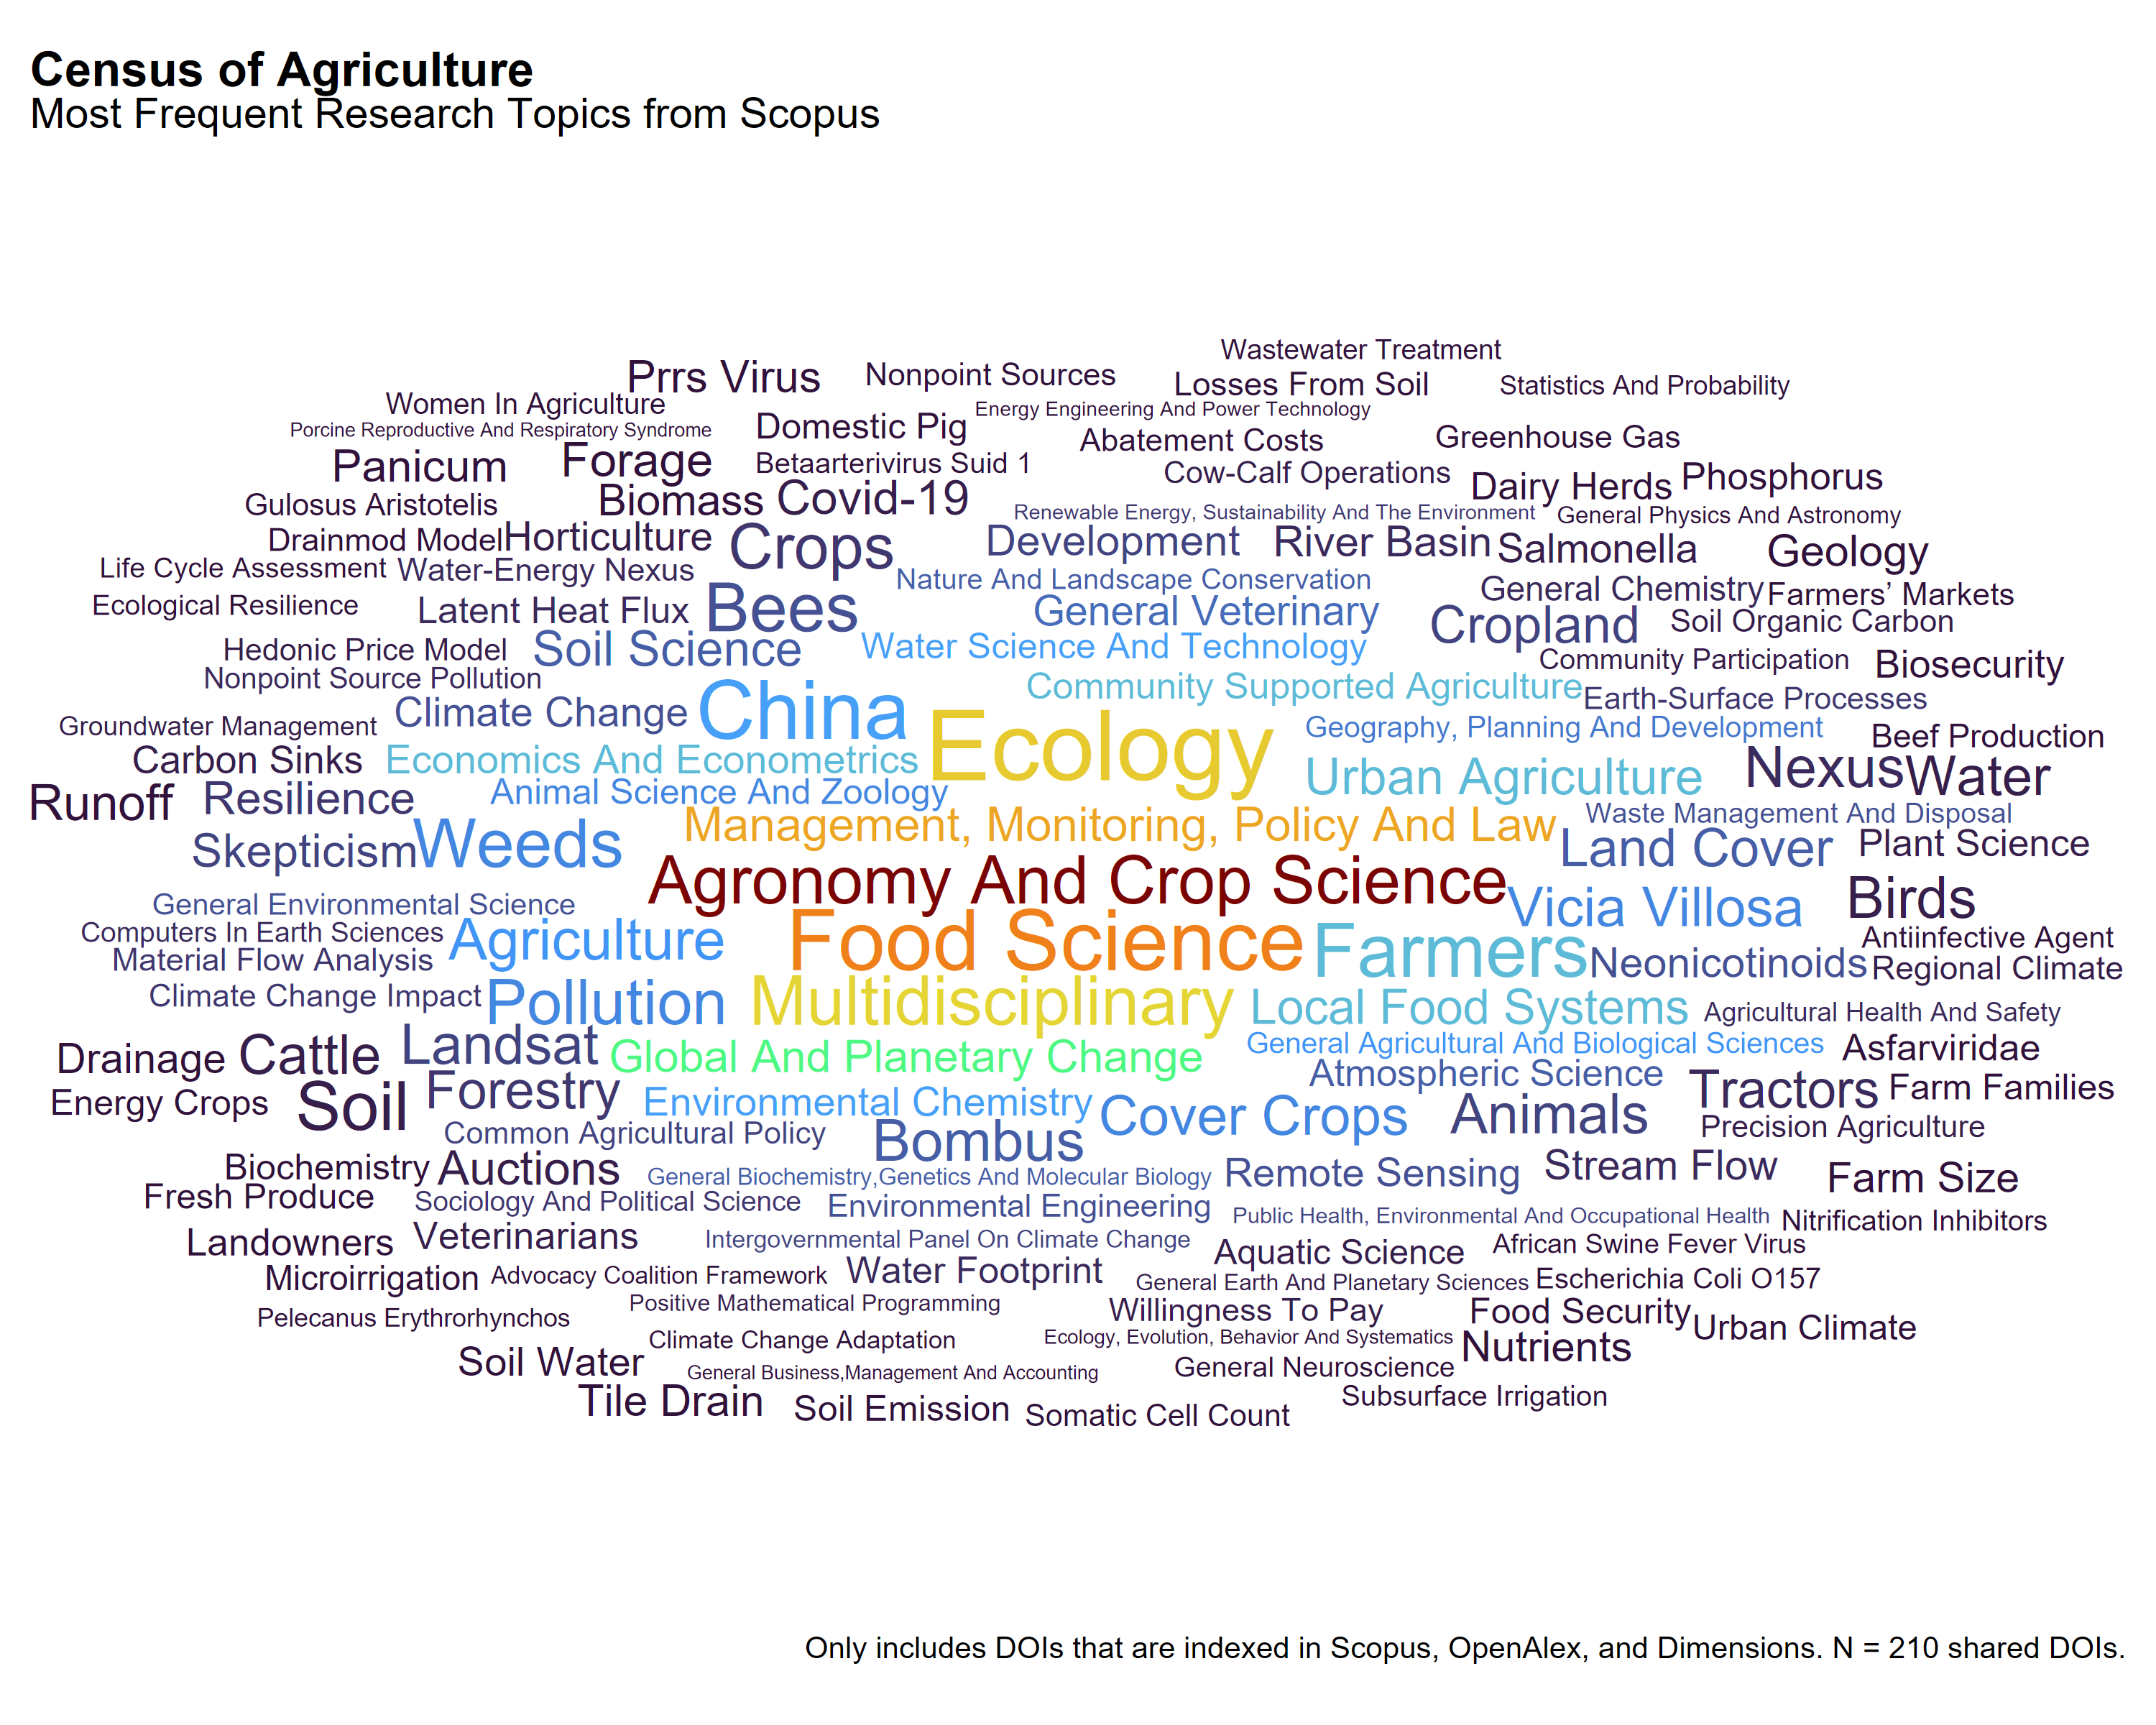
\includegraphics[keepaspectratio]{graphics/word_clouds/shared_dois/dataset05_wordcloud_shared_scopus.png}}

\paragraph{OpenAlex}

\pandocbounded{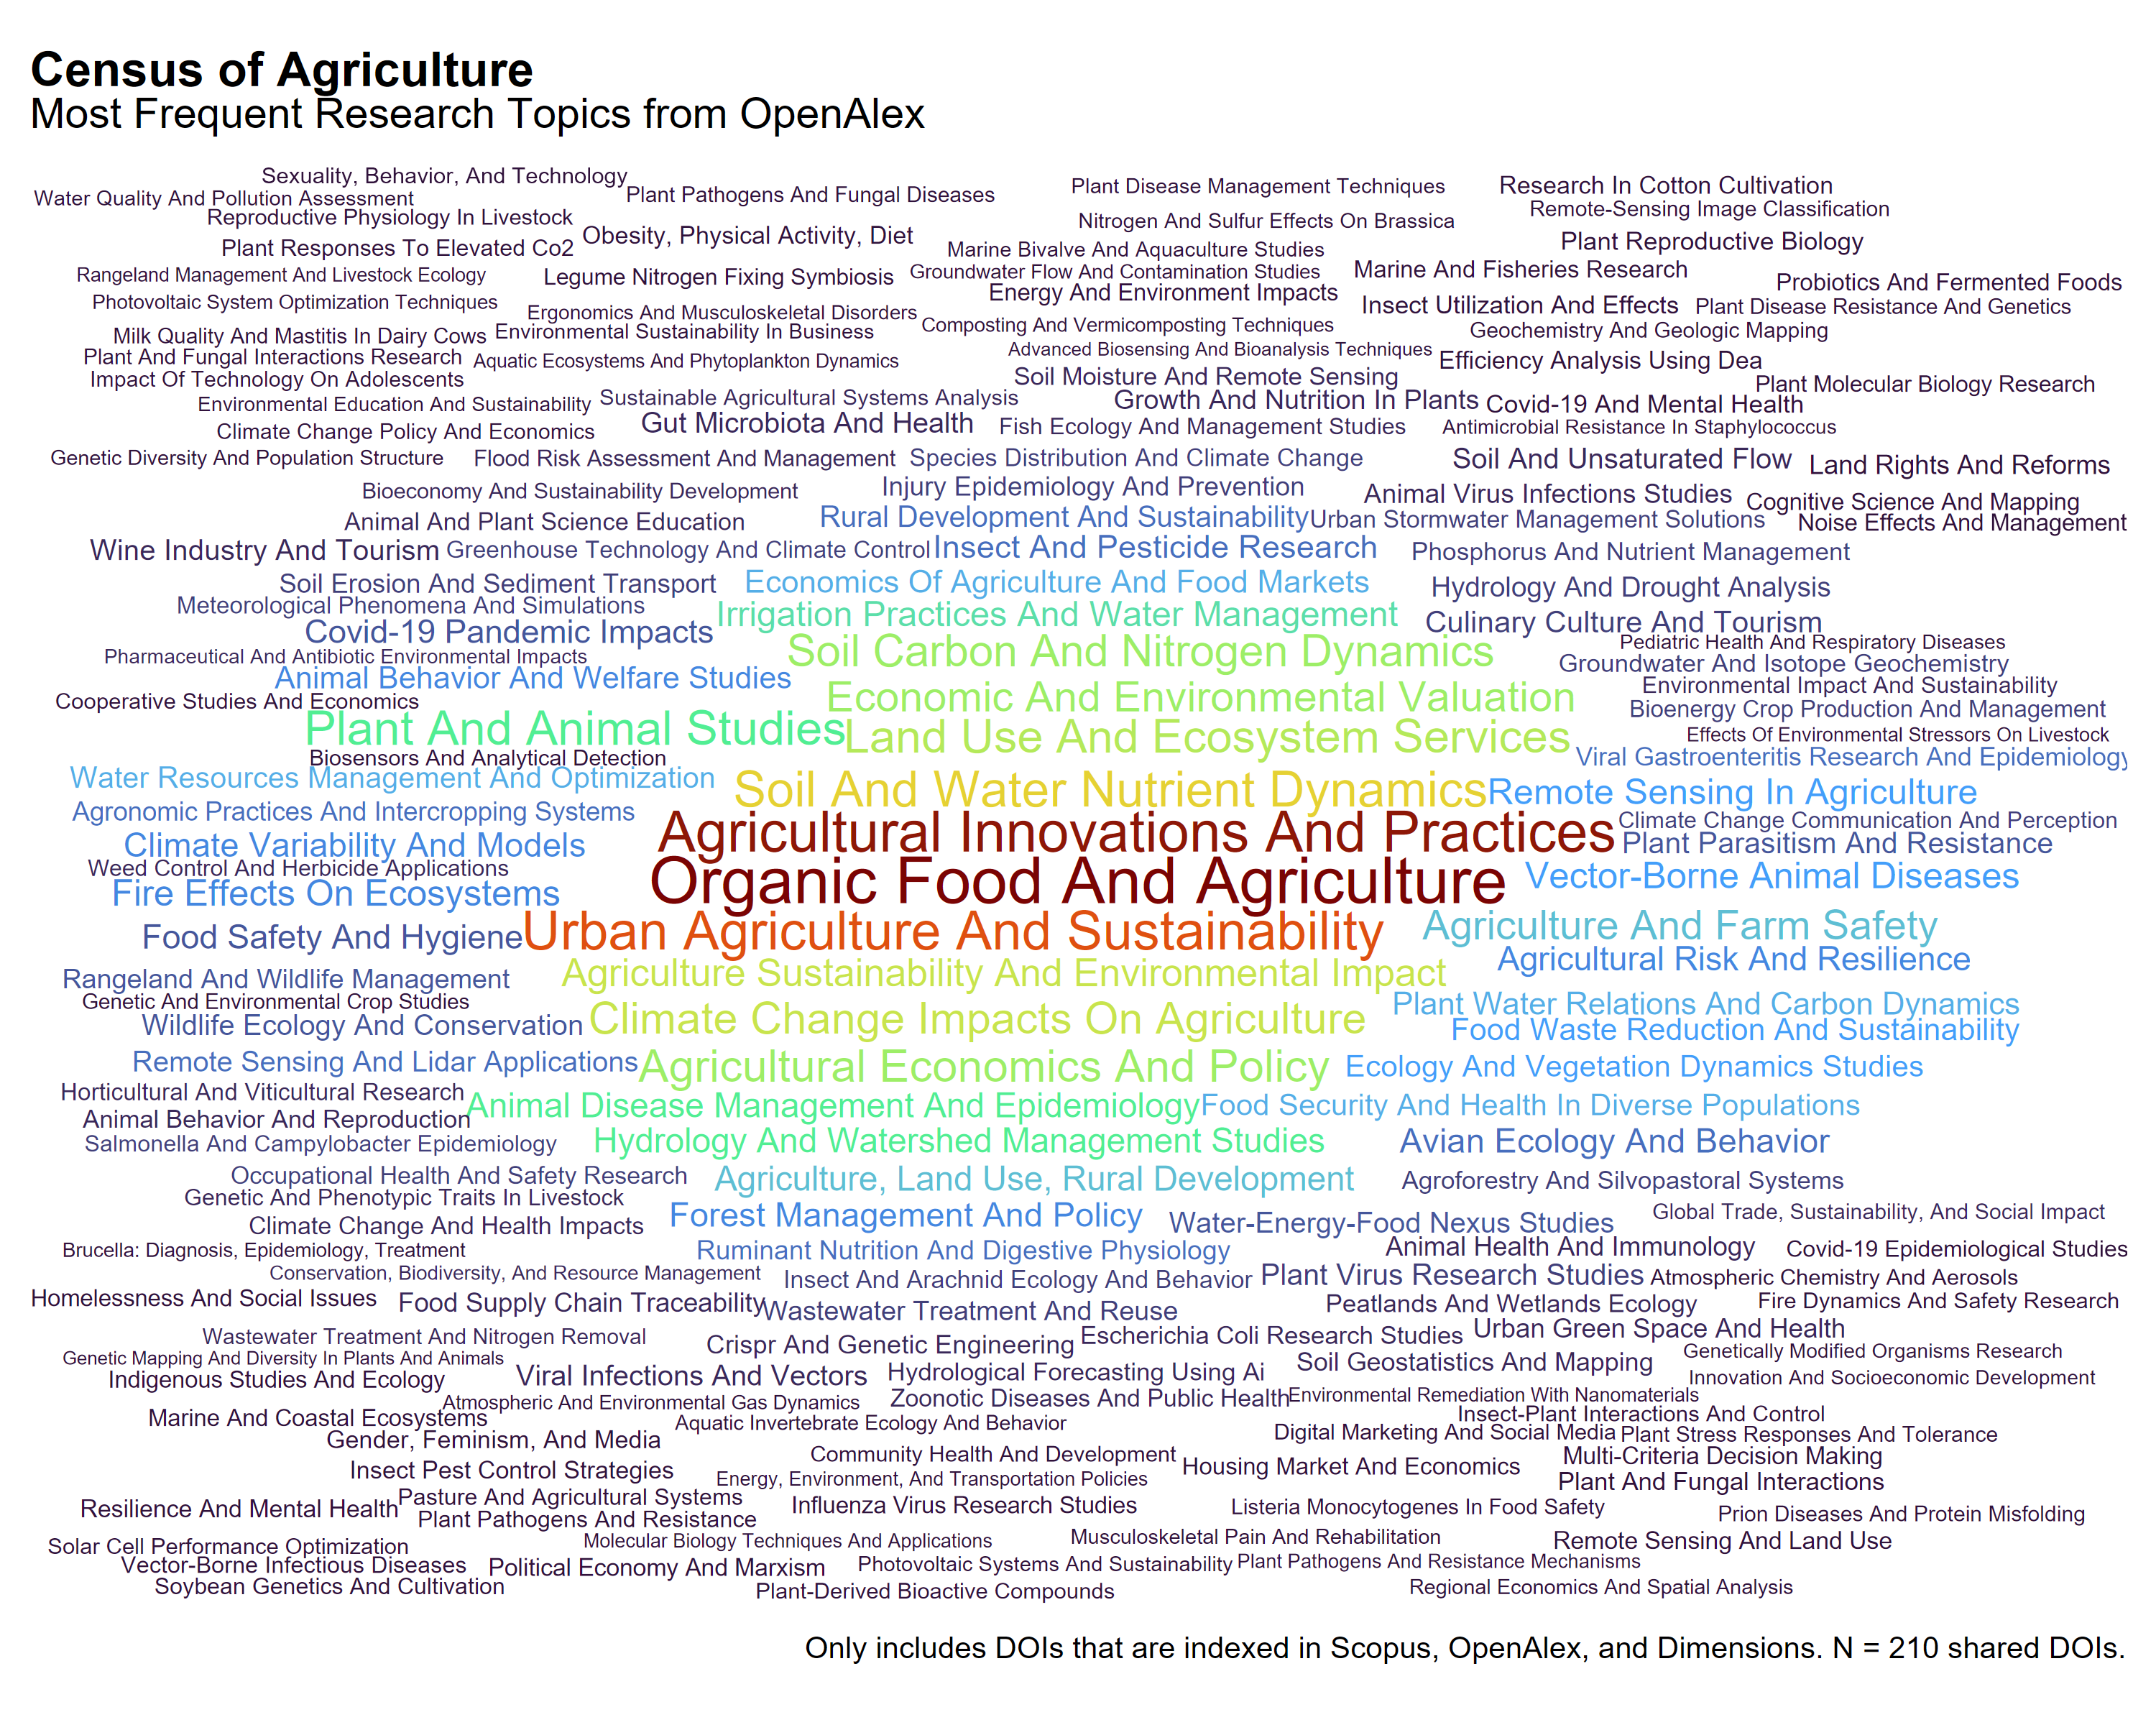
\includegraphics[keepaspectratio]{graphics/word_clouds/shared_dois/dataset05_wordcloud_shared_openalex.png}}

\paragraph{Dimensions}

\pandocbounded{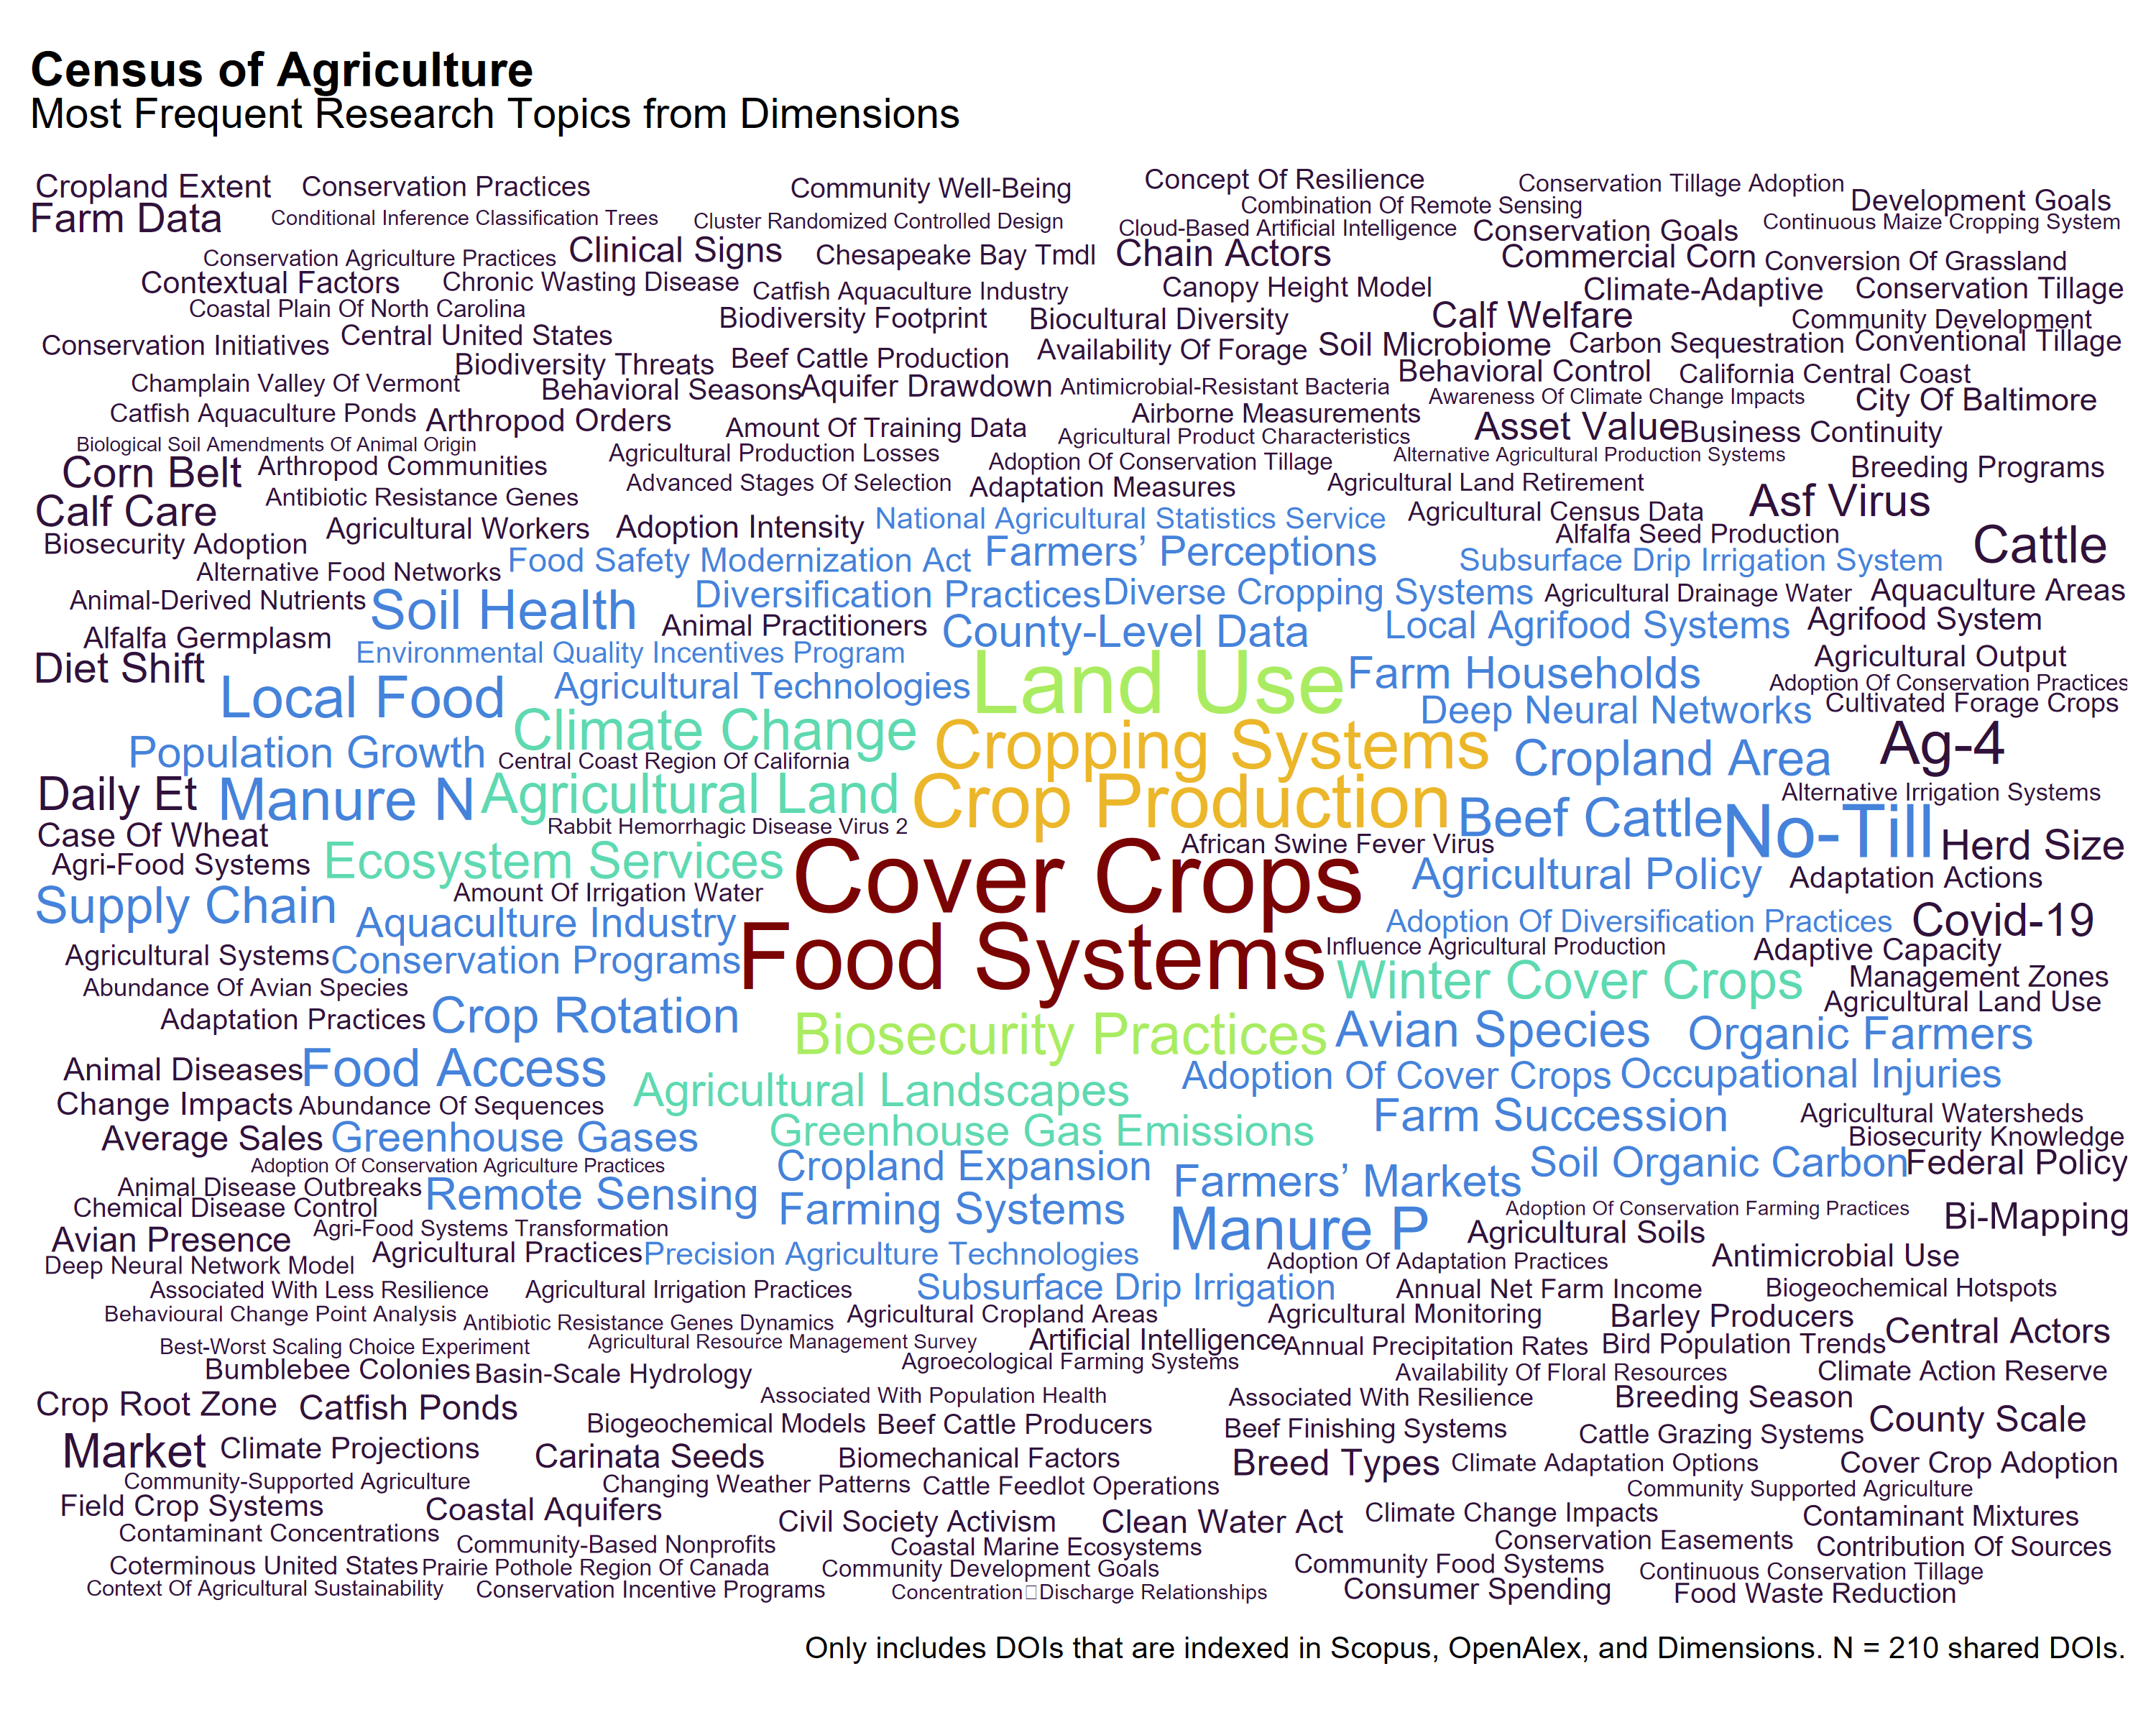
\includegraphics[keepaspectratio]{graphics/word_clouds/shared_dois/dataset05_wordcloud_shared_dimensions.png}}

The next set of word clouds summarizes the most frequent research topics
associated with publications that reference a given dataset, based on
each source's topic classification schema. The first word cloud in each
section aggregates topics across all sources---Scopus, OpenAlex, and
Dimensions---to provide a composite view of the research landscape.
Readers can then click on source-specific word clouds, which reflect the
full corpus of DOIs referencing the dataset within each source. These
differences highlight how each platform categorizes scholarly content
and may inform decisions about dataset visibility and disciplinary
reach.

\begin{tcolorbox}[enhanced jigsaw, leftrule=.75mm, colframe=quarto-callout-note-color-frame, toprule=.15mm, titlerule=0mm, colback=white, rightrule=.15mm, opacityback=0, breakable, bottomtitle=1mm, coltitle=black, colbacktitle=quarto-callout-note-color!10!white, left=2mm, toptitle=1mm, opacitybacktitle=0.6, title=\textcolor{quarto-callout-note-color}{\faInfo}\hspace{0.5em}{Additional Word Cloud Variants}, arc=.35mm, bottomrule=.15mm]

\end{tcolorbox}

\paragraph*{Food Access Research
Atlas}\label{food-access-research-atlas-2}
\addcontentsline{toc}{paragraph}{Food Access Research Atlas}

For the 65 publications indexed across Scopus, OpenAlex, and Dimensions
that reference the Food Access Research Atlas, topic classifications
vary by source. Each database reflects different emphases in how it
organizes subject matter related to food environments and
neighborhood-level access.

Dimensions highlights terms associated with food insecurity and
nutrition assistance, including Food Deserts, Food Insecurity, SNAP
Participants, and Census Tracts. The topics are often grounded in
program participation, geographic mapping, and diet-related outcomes,
suggesting an applied framing centered on public policy and access
programs.

OpenAlex points to broader social and environmental determinants of
health, with topics like Obesity, Physical Activity, Diet, Food Security
and Health in Diverse Populations, and Urban Agriculture and
Sustainability. Its classifications suggest greater integration of
population health, urban studies, and structural considerations.

Scopus displays a mix of disciplinary and clinical topics, including
Obesity, Grocery Stores, Farmers' Markets, and Public Health. Additional
terms such as Anthropology, Exercise, Surgery, and Biomedical
Engineering reflect coverage from journals in the health sciences,
indicating a more biomedical orientation.

Together, these differences suggest that Dimensions frames FARA-related
research through the lens of policy and programmatic access, OpenAlex
places greater emphasis on social context and urban health, and Scopus
reflects disciplinary classifications from medicine, biology, and public
health. These variations may influence how different audiences encounter
and interpret research using this dataset.

\paragraph{Scopus}

\pandocbounded{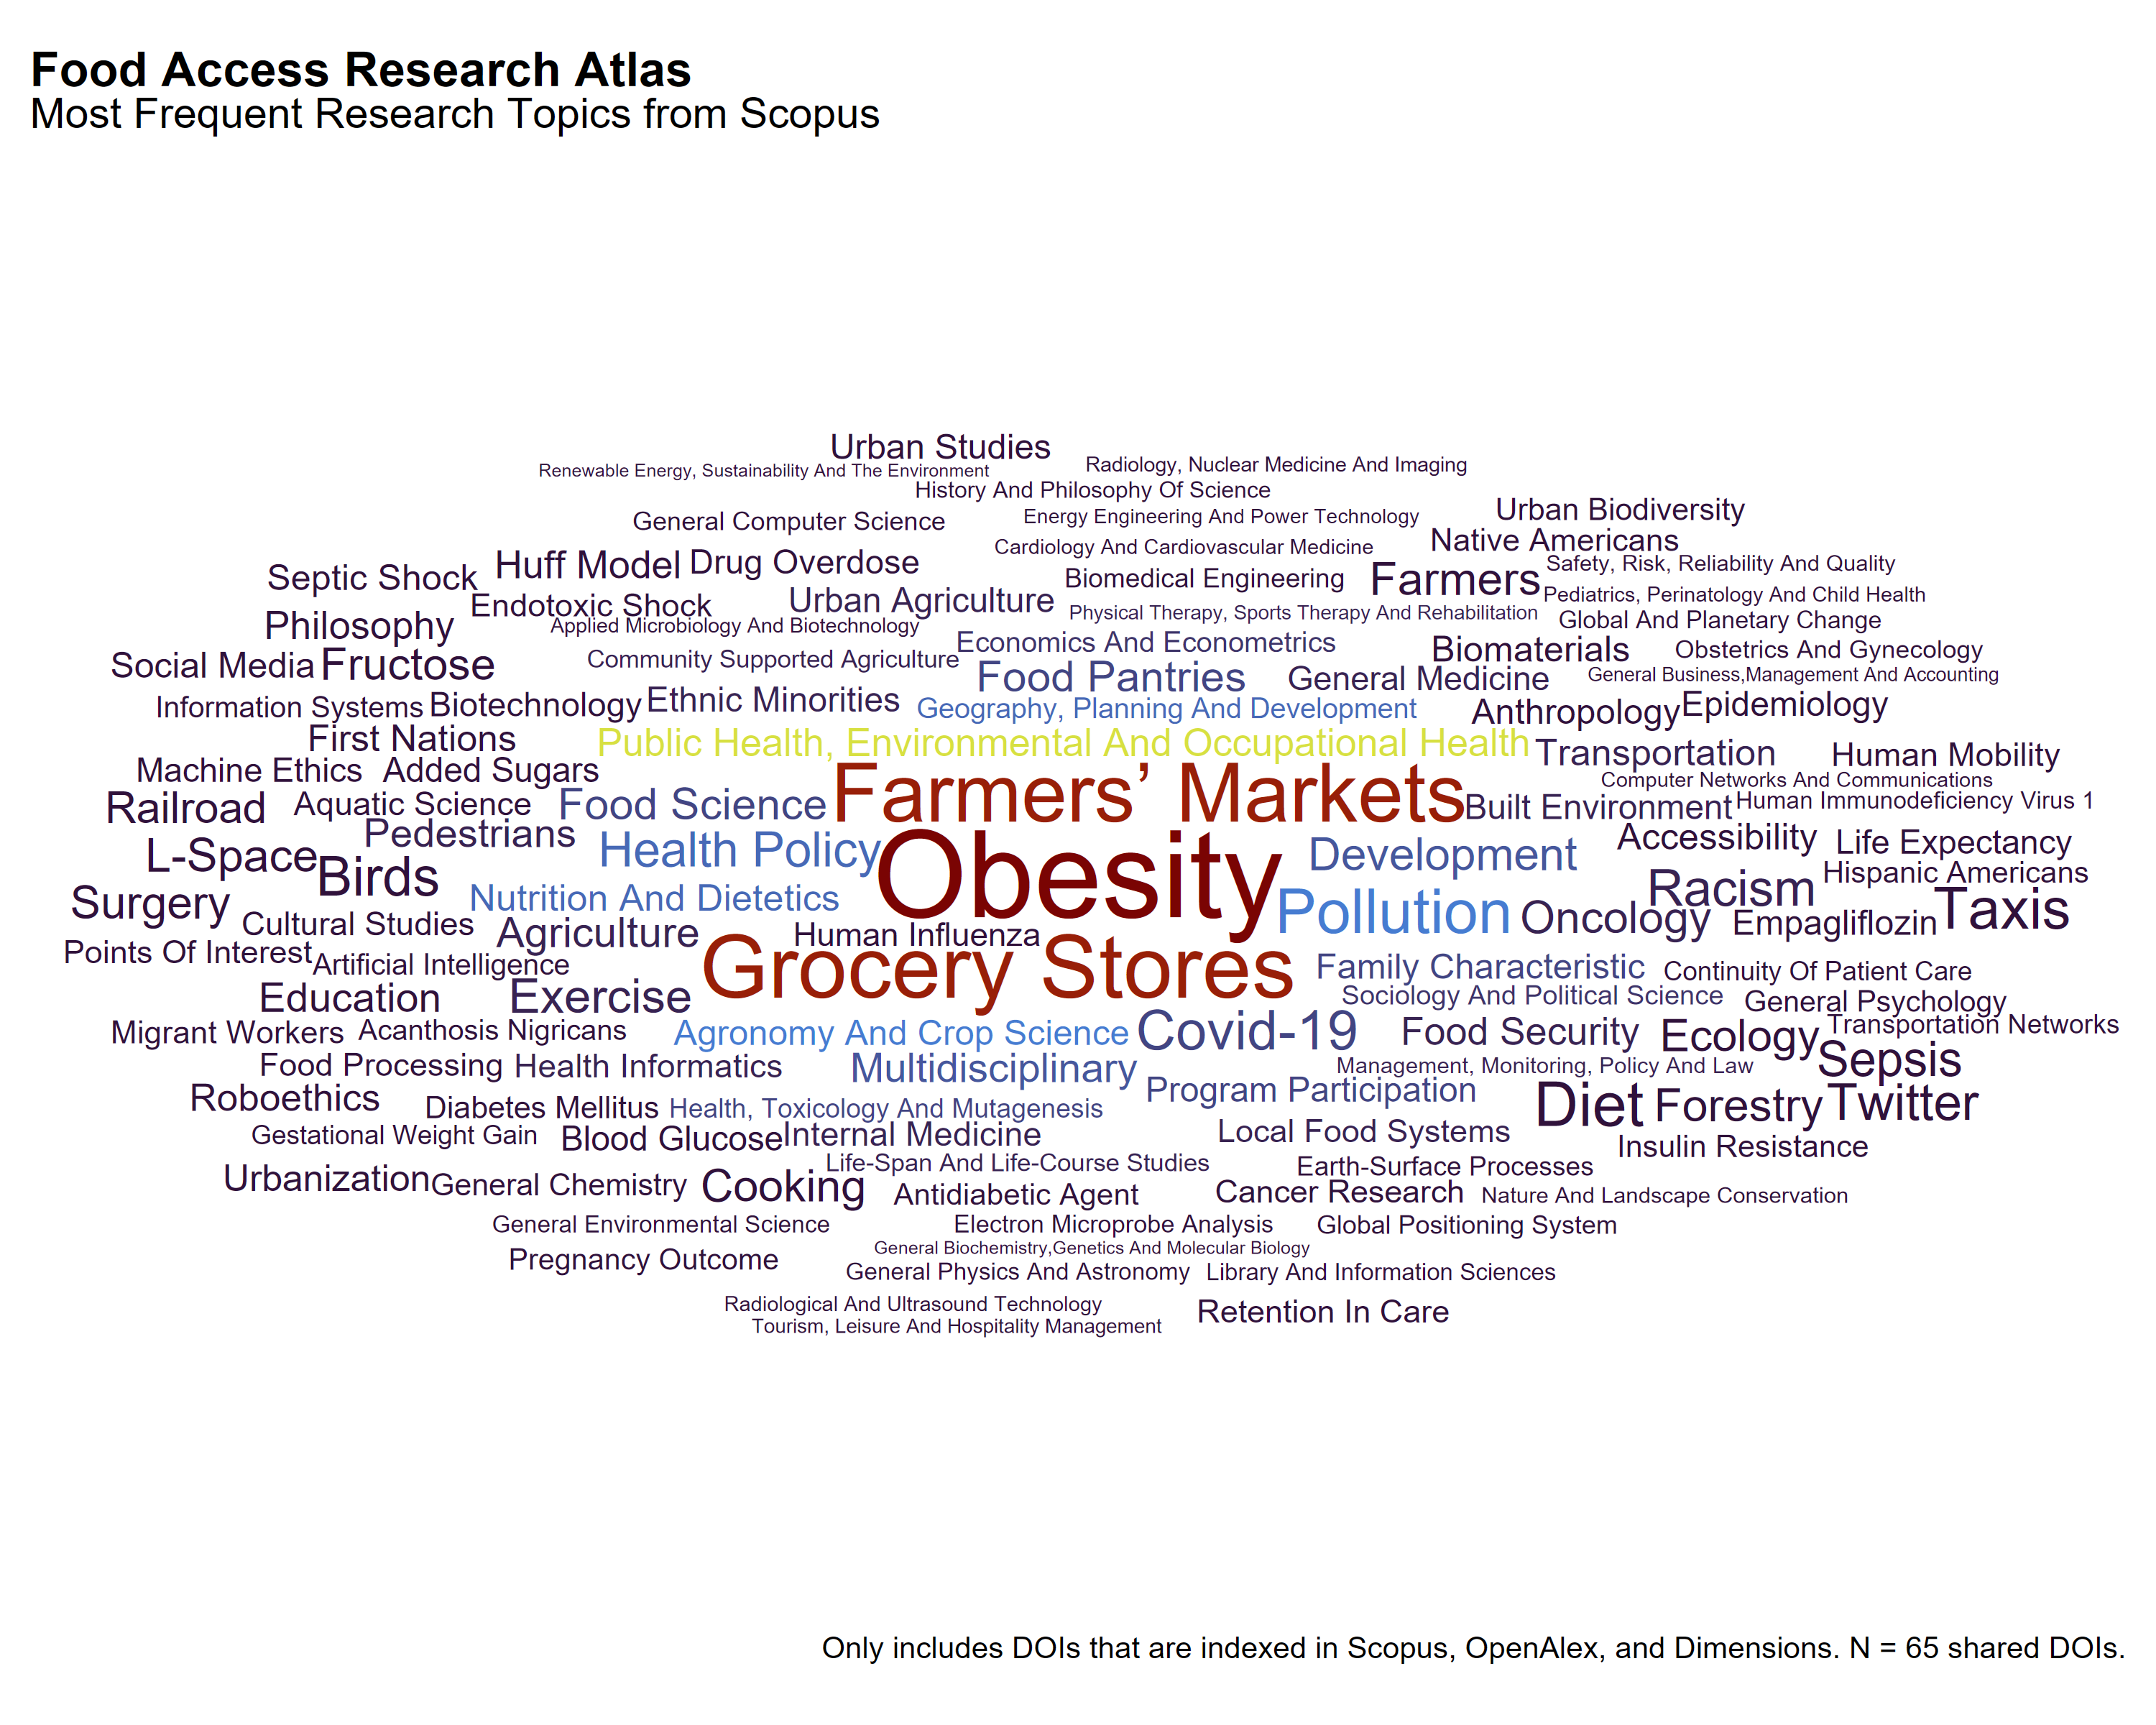
\includegraphics[keepaspectratio]{graphics/word_clouds/shared_dois/dataset08_wordcloud_shared_scopus.png}}

\paragraph{OpenAlex}

\pandocbounded{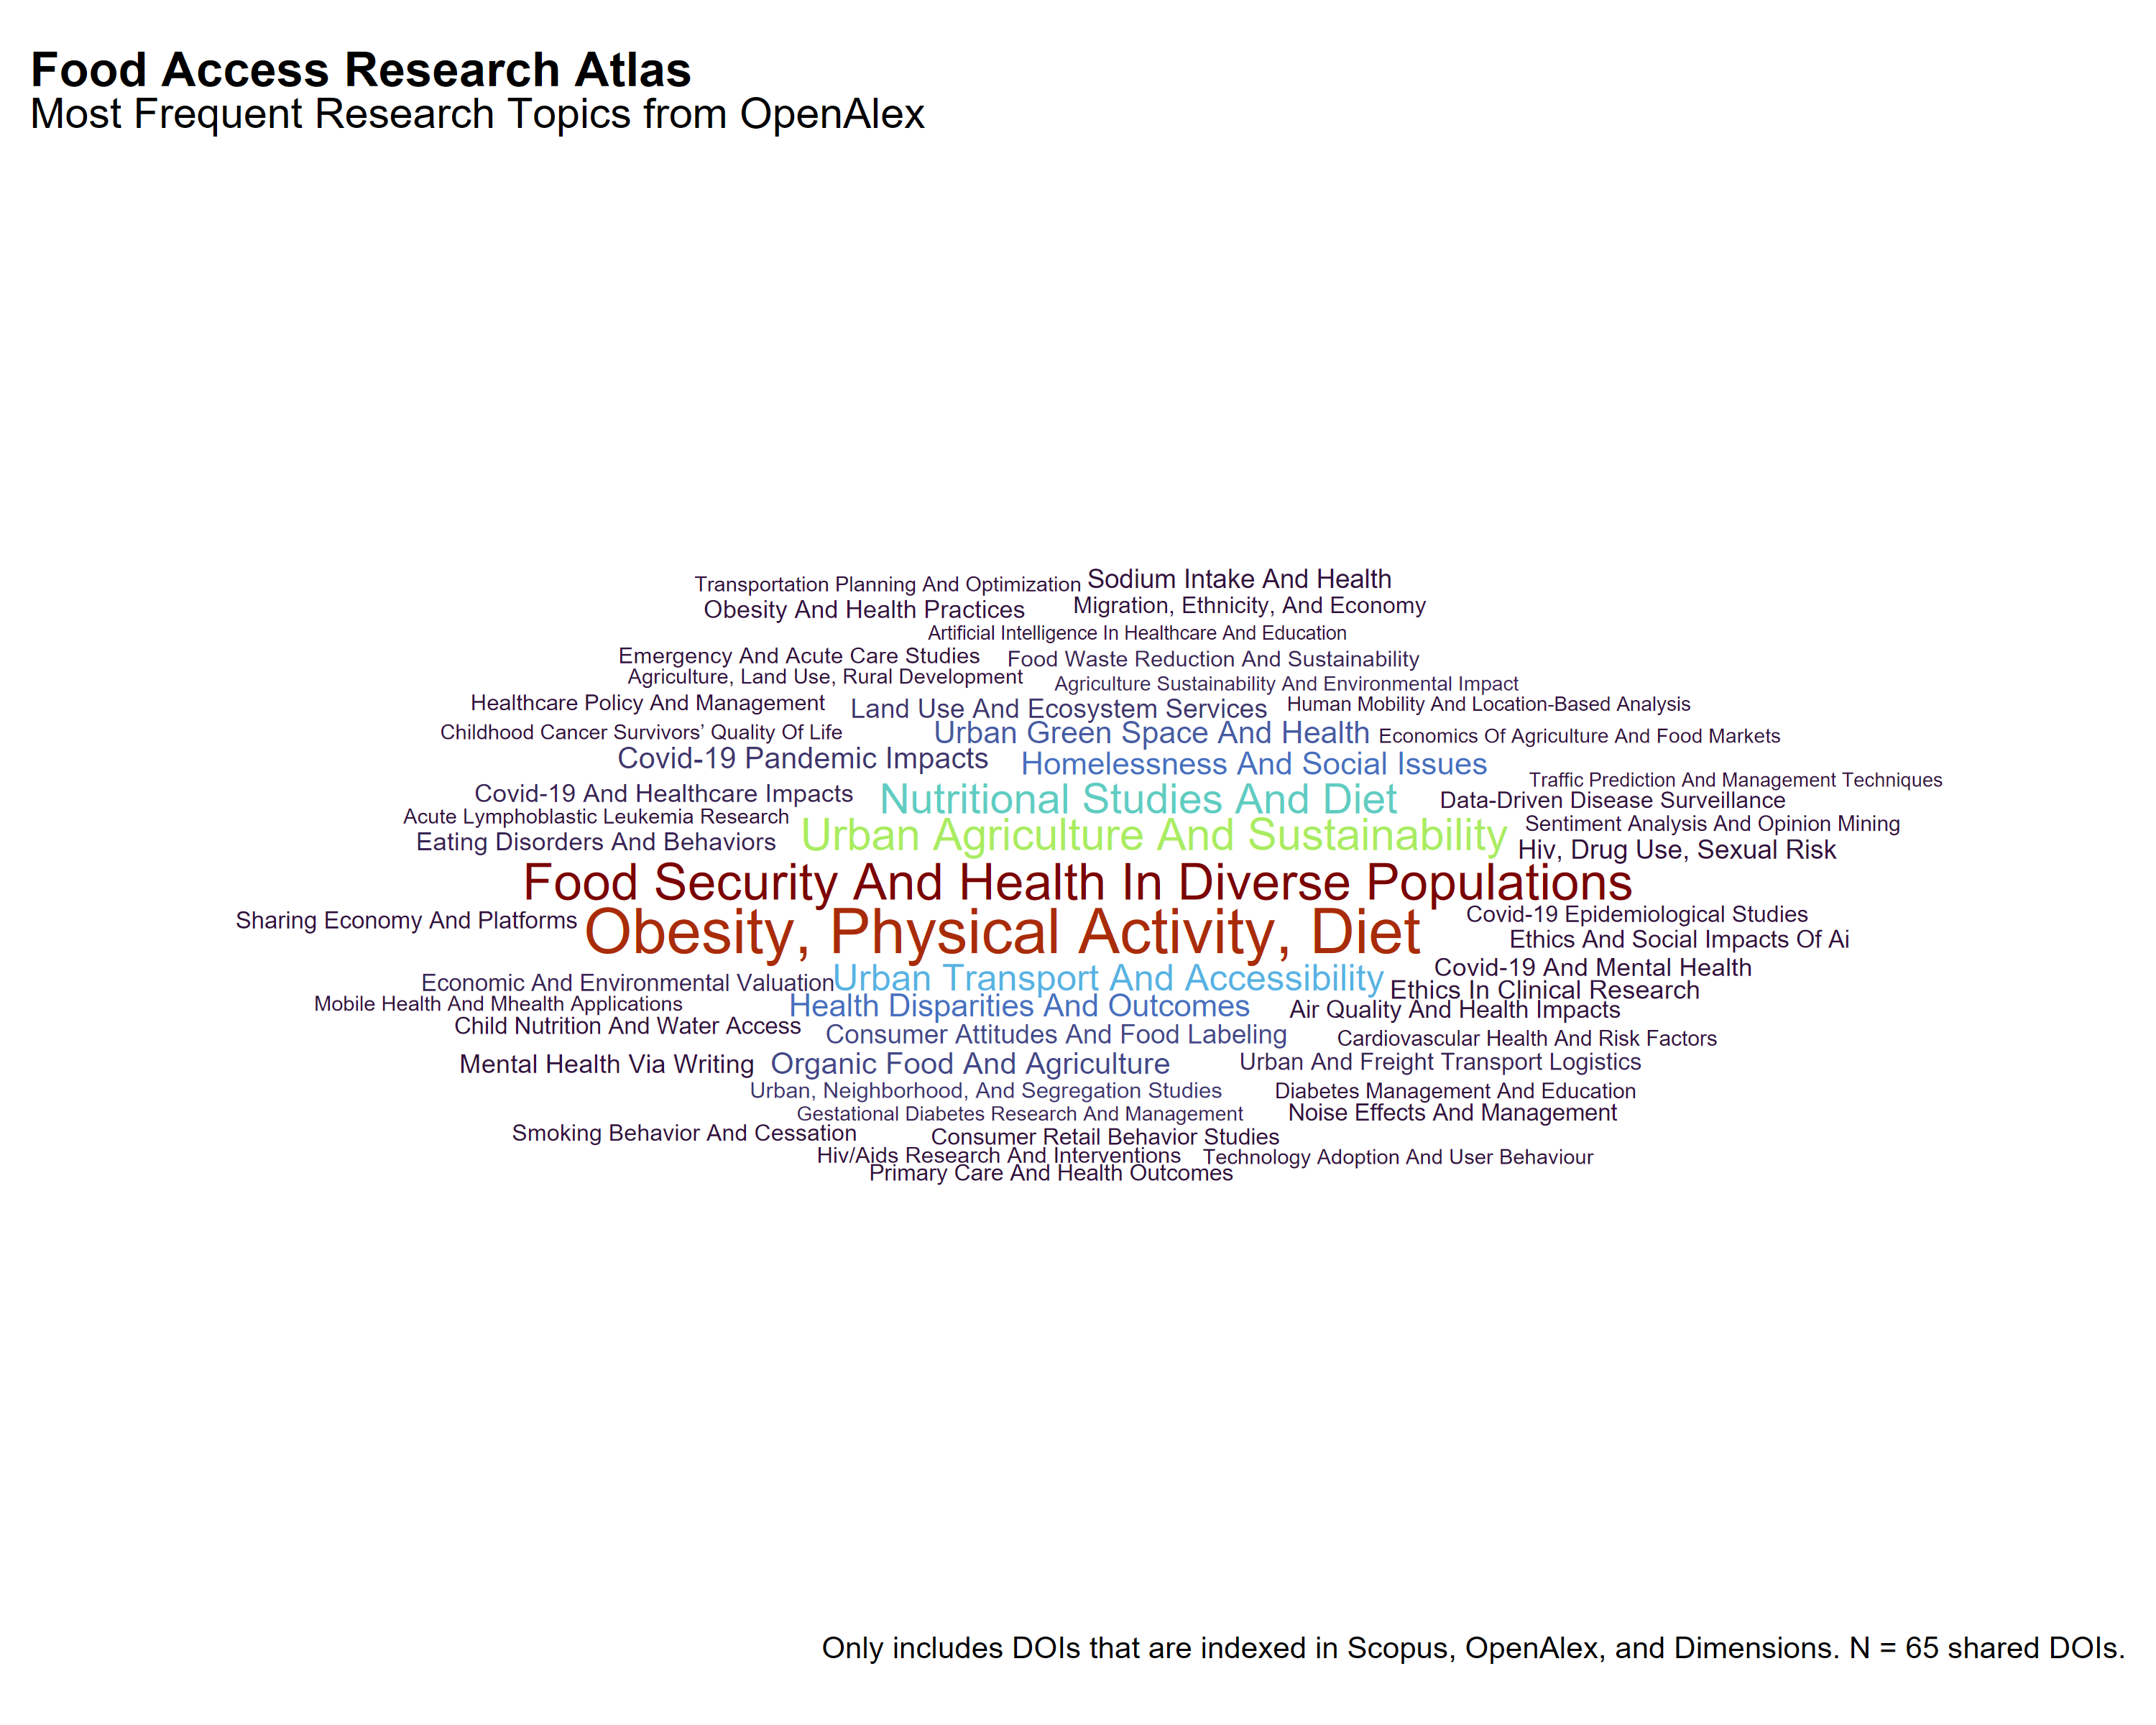
\includegraphics[keepaspectratio]{graphics/word_clouds/shared_dois/dataset08_wordcloud_shared_openalex.png}}

\paragraph{Dimensions}

\pandocbounded{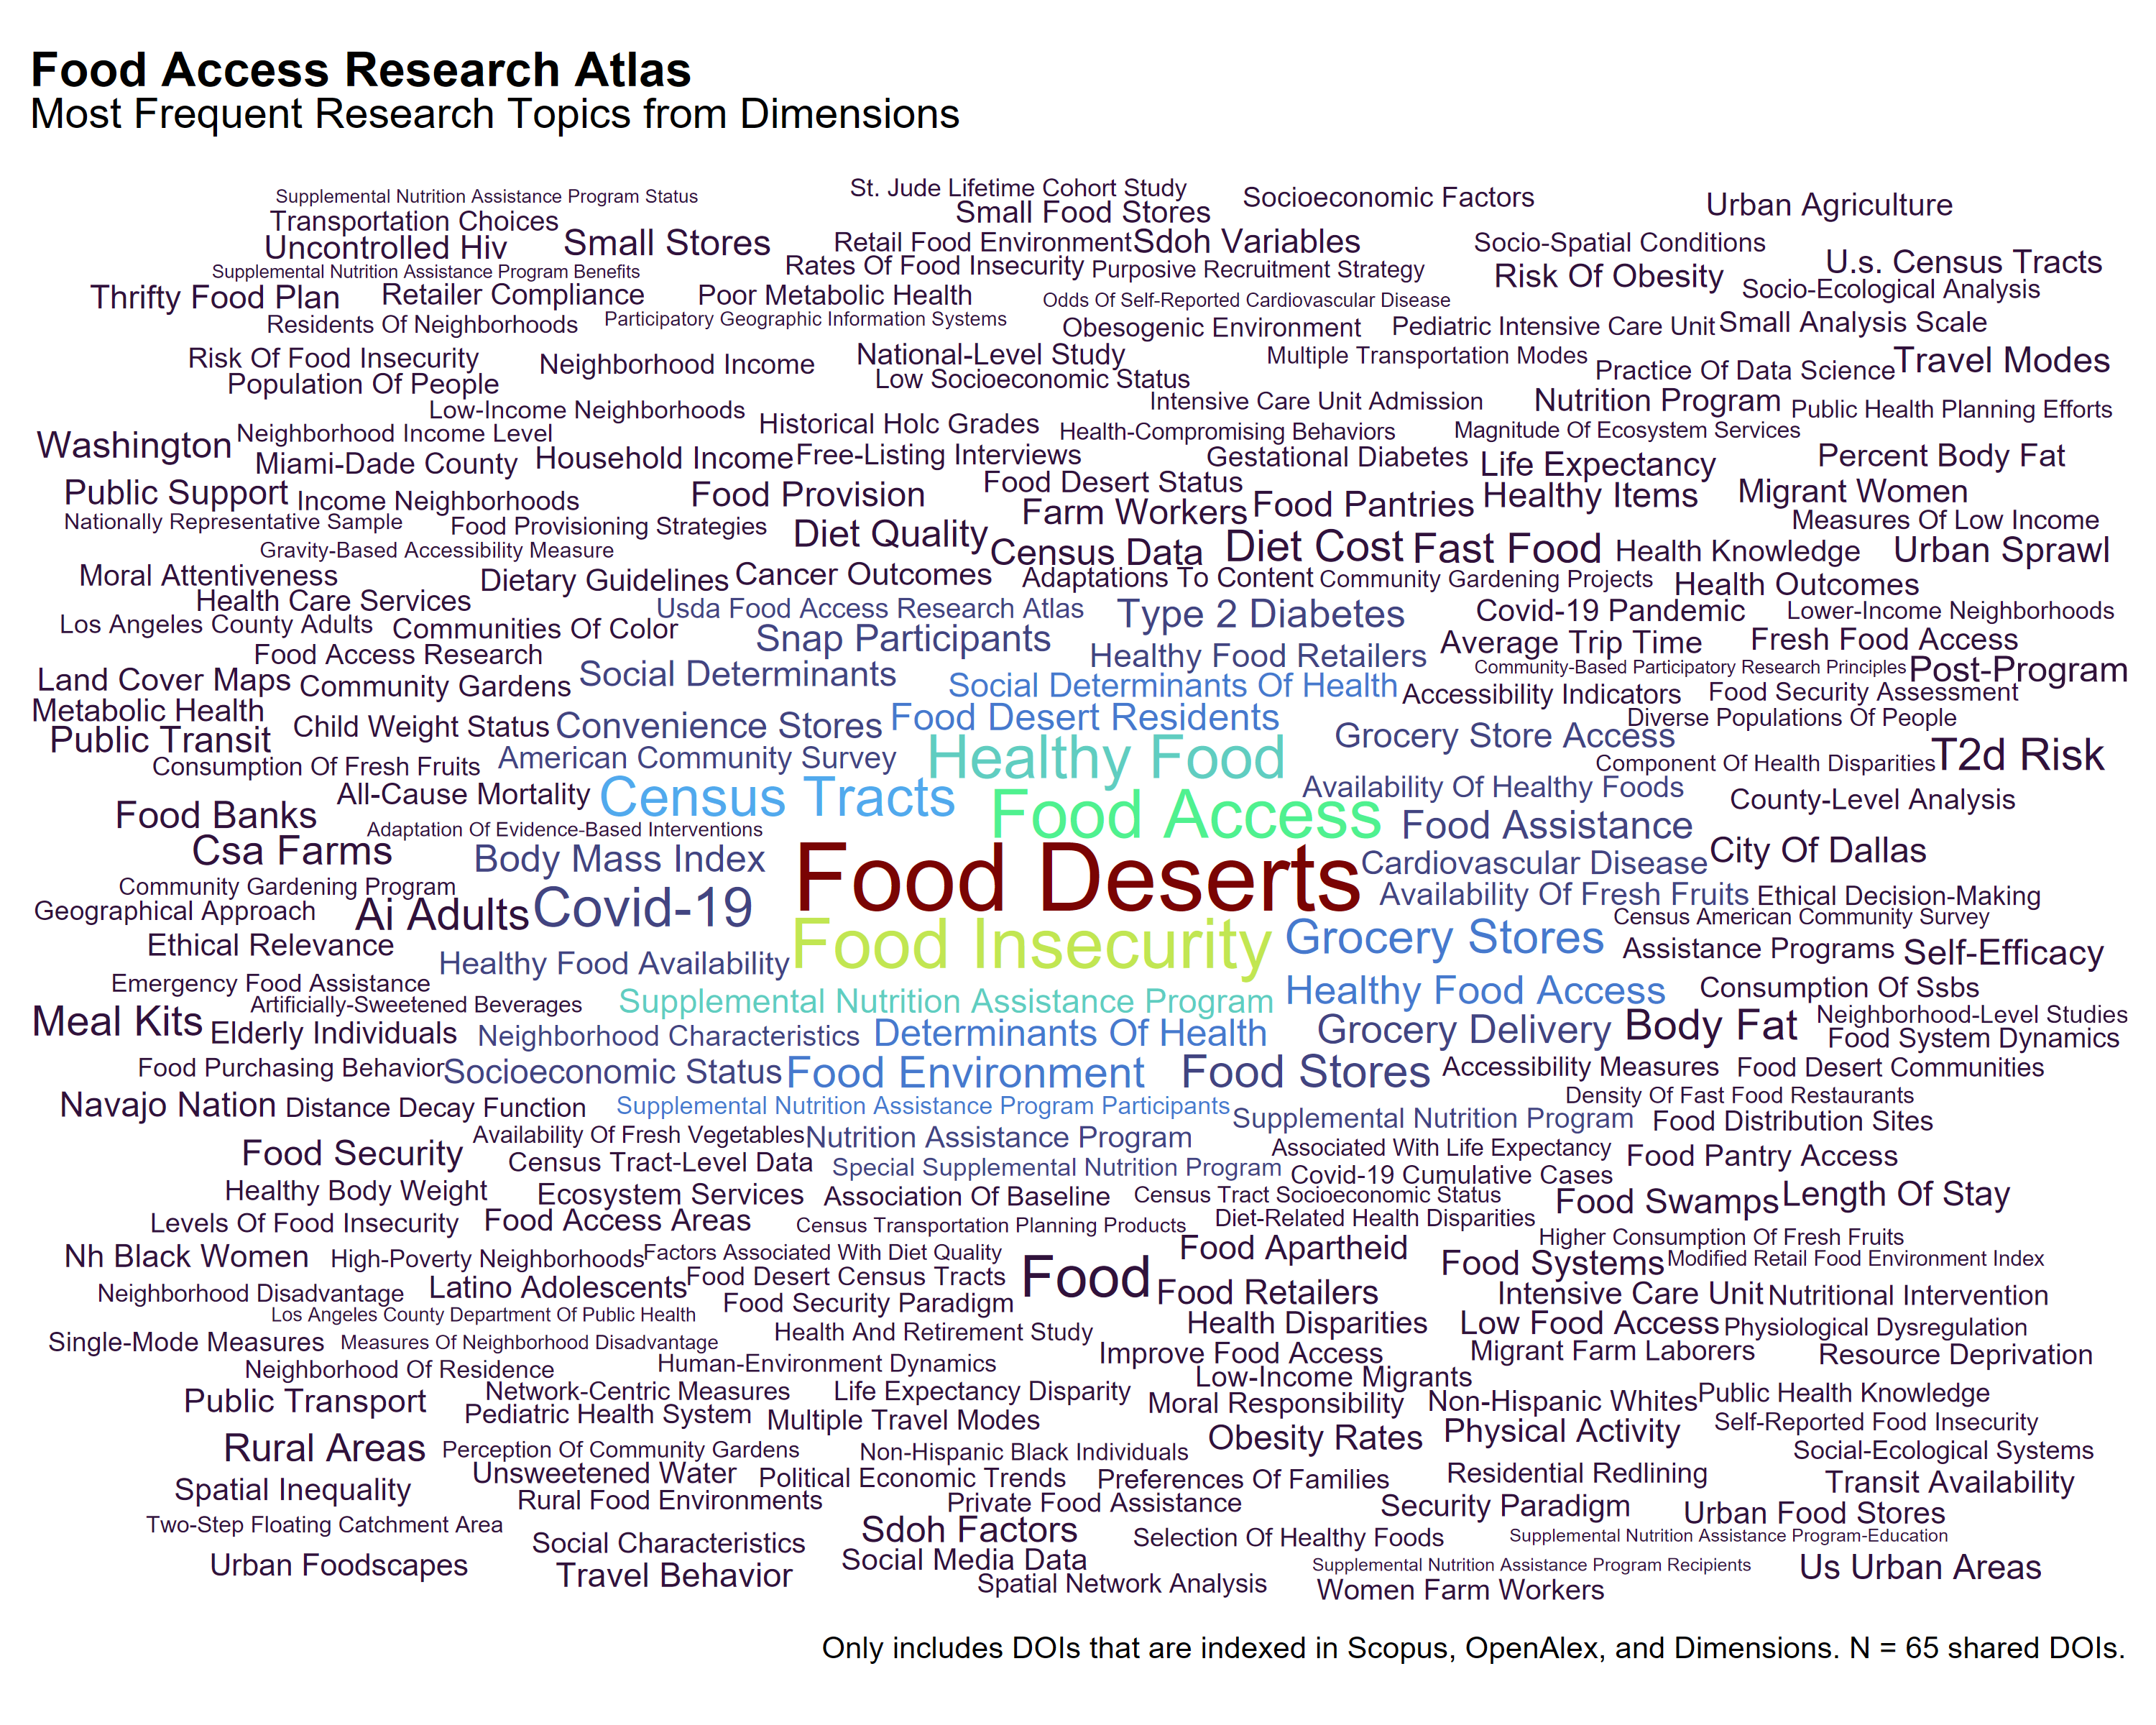
\includegraphics[keepaspectratio]{graphics/word_clouds/shared_dois/dataset08_wordcloud_shared_dimensions.png}}

The next set of word clouds summarizes the most frequent research topics
associated with publications that reference a given dataset, based on
each source's topic classification schema. The first word cloud in each
section aggregates topics across all sources---Scopus, OpenAlex, and
Dimensions---to provide a composite view of the research landscape.
Readers can then click on source-specific word clouds, which reflect the
full corpus of DOIs referencing the dataset within each source. These
differences highlight how each platform categorizes scholarly content
and may inform decisions about dataset visibility and disciplinary
reach.

\begin{tcolorbox}[enhanced jigsaw, leftrule=.75mm, colframe=quarto-callout-note-color-frame, toprule=.15mm, titlerule=0mm, colback=white, rightrule=.15mm, opacityback=0, breakable, bottomtitle=1mm, coltitle=black, colbacktitle=quarto-callout-note-color!10!white, left=2mm, toptitle=1mm, opacitybacktitle=0.6, title=\textcolor{quarto-callout-note-color}{\faInfo}\hspace{0.5em}{Additional Word Cloud Variants}, arc=.35mm, bottomrule=.15mm]

\end{tcolorbox}

\paragraph*{The Food Acquisition and Purchase Survey
(FoodAPS)}\label{the-food-acquisition-and-purchase-survey-foodaps-2}
\addcontentsline{toc}{paragraph}{The Food Acquisition and Purchase
Survey (FoodAPS)}

Among the 38 DOIs referencing FoodAPS that appear in all three citation
databases, each source assigns different topic labels, offering varied
perspectives on the dataset's use in scholarly research.

Dimensions emphasizes topics directly connected to food purchasing and
economic access. Prominent terms include Diet Cost, Food Environment,
Thrifty Food Plan, and Supplemental Nutrition Assistance Program. These
labels reflect applied work related to food affordability, policy
programs, and nutrition behavior, often at the household level.

OpenAlex highlights broader public health themes such as Obesity,
Physical Activity, Diet and Food Security and Health in Diverse
Populations. It also includes terms related to structural and behavioral
contexts---Urban Agriculture and Sustainability, Homelessness and Social
Issues, and Consumer Attitudes and Food Labeling---suggesting a focus on
population-level outcomes and intersectional influences on food access.

Scopus shows more disciplinary and intervention-related topics. Terms
like Grocery Stores, Farmers' Markets, Nutrition and Dietetics, and
Obesity appear frequently, alongside topics such as Brand Placement,
Food Labeling, and Program Participation, indicating interest in
behavioral nutrition, food marketing, and policy evaluation.

These differences suggest that Dimensions favors classification by
programmatic and economic relevance, OpenAlex aligns more with public
health and social research, and Scopus tends to organize around
disciplinary domains and evaluation studies.

\paragraph{Scopus}

\pandocbounded{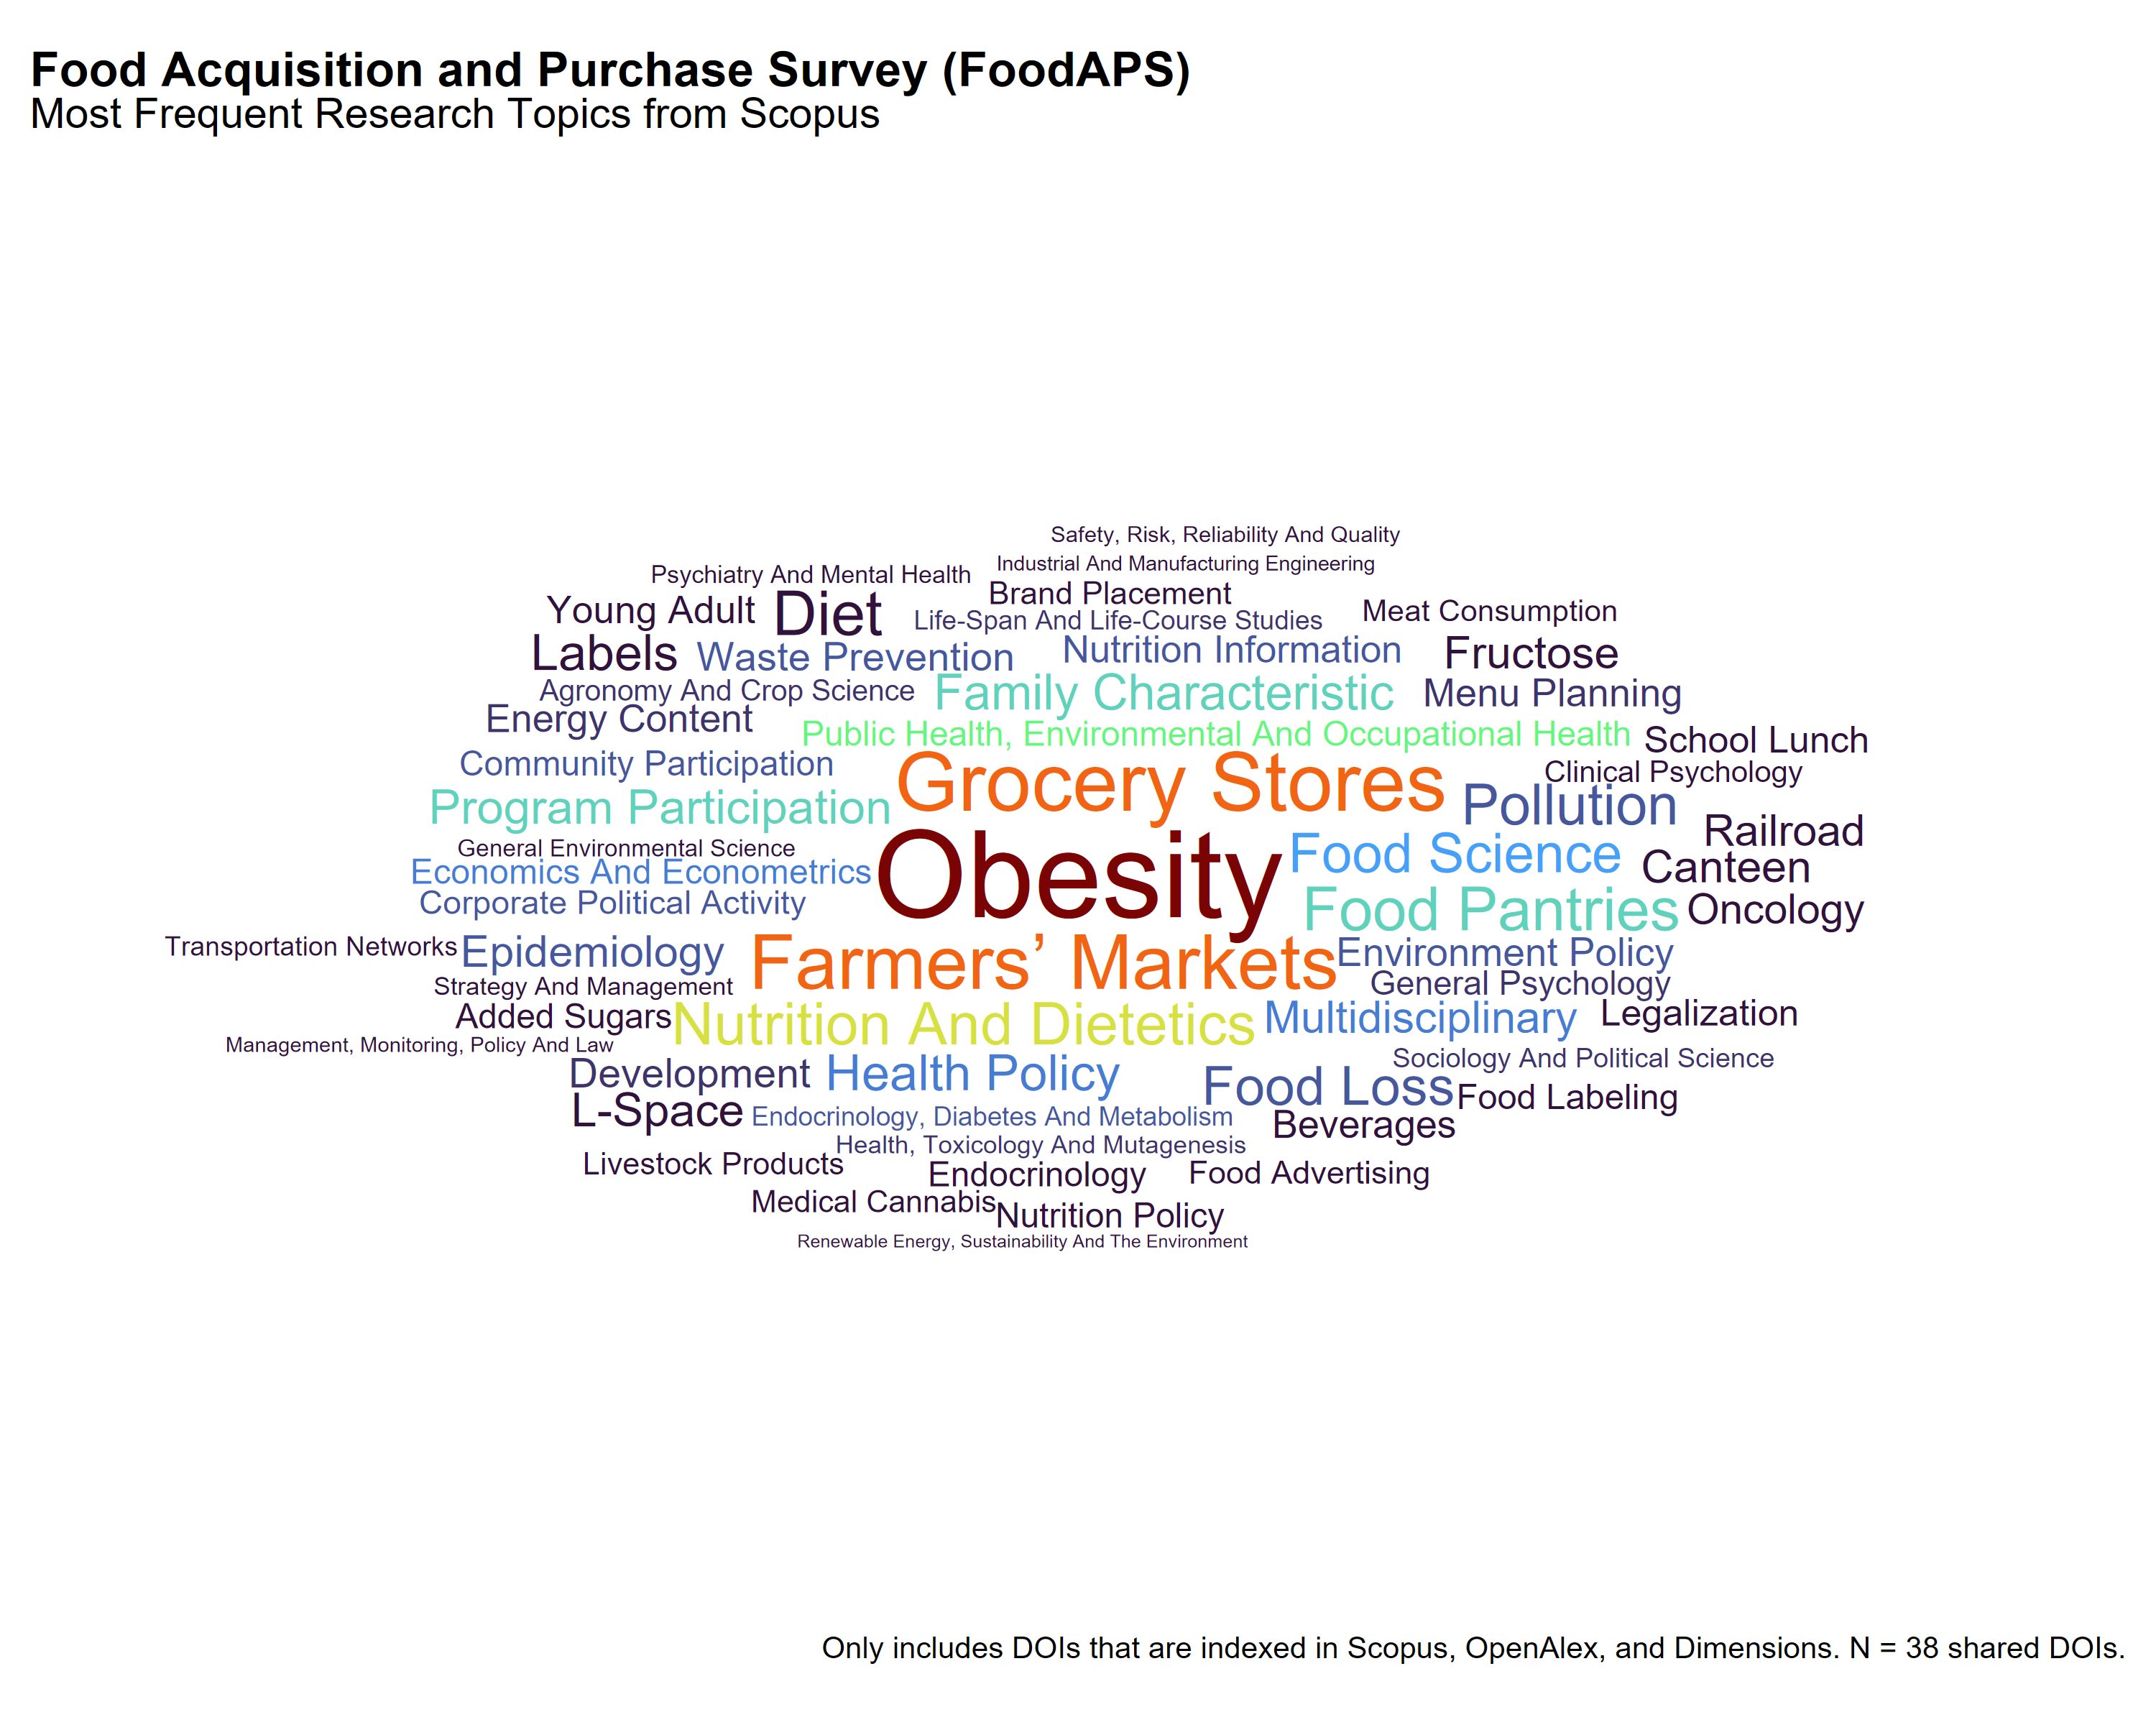
\includegraphics[keepaspectratio]{graphics/word_clouds/shared_dois/dataset09_wordcloud_shared_scopus.png}}

\paragraph{OpenAlex}

\pandocbounded{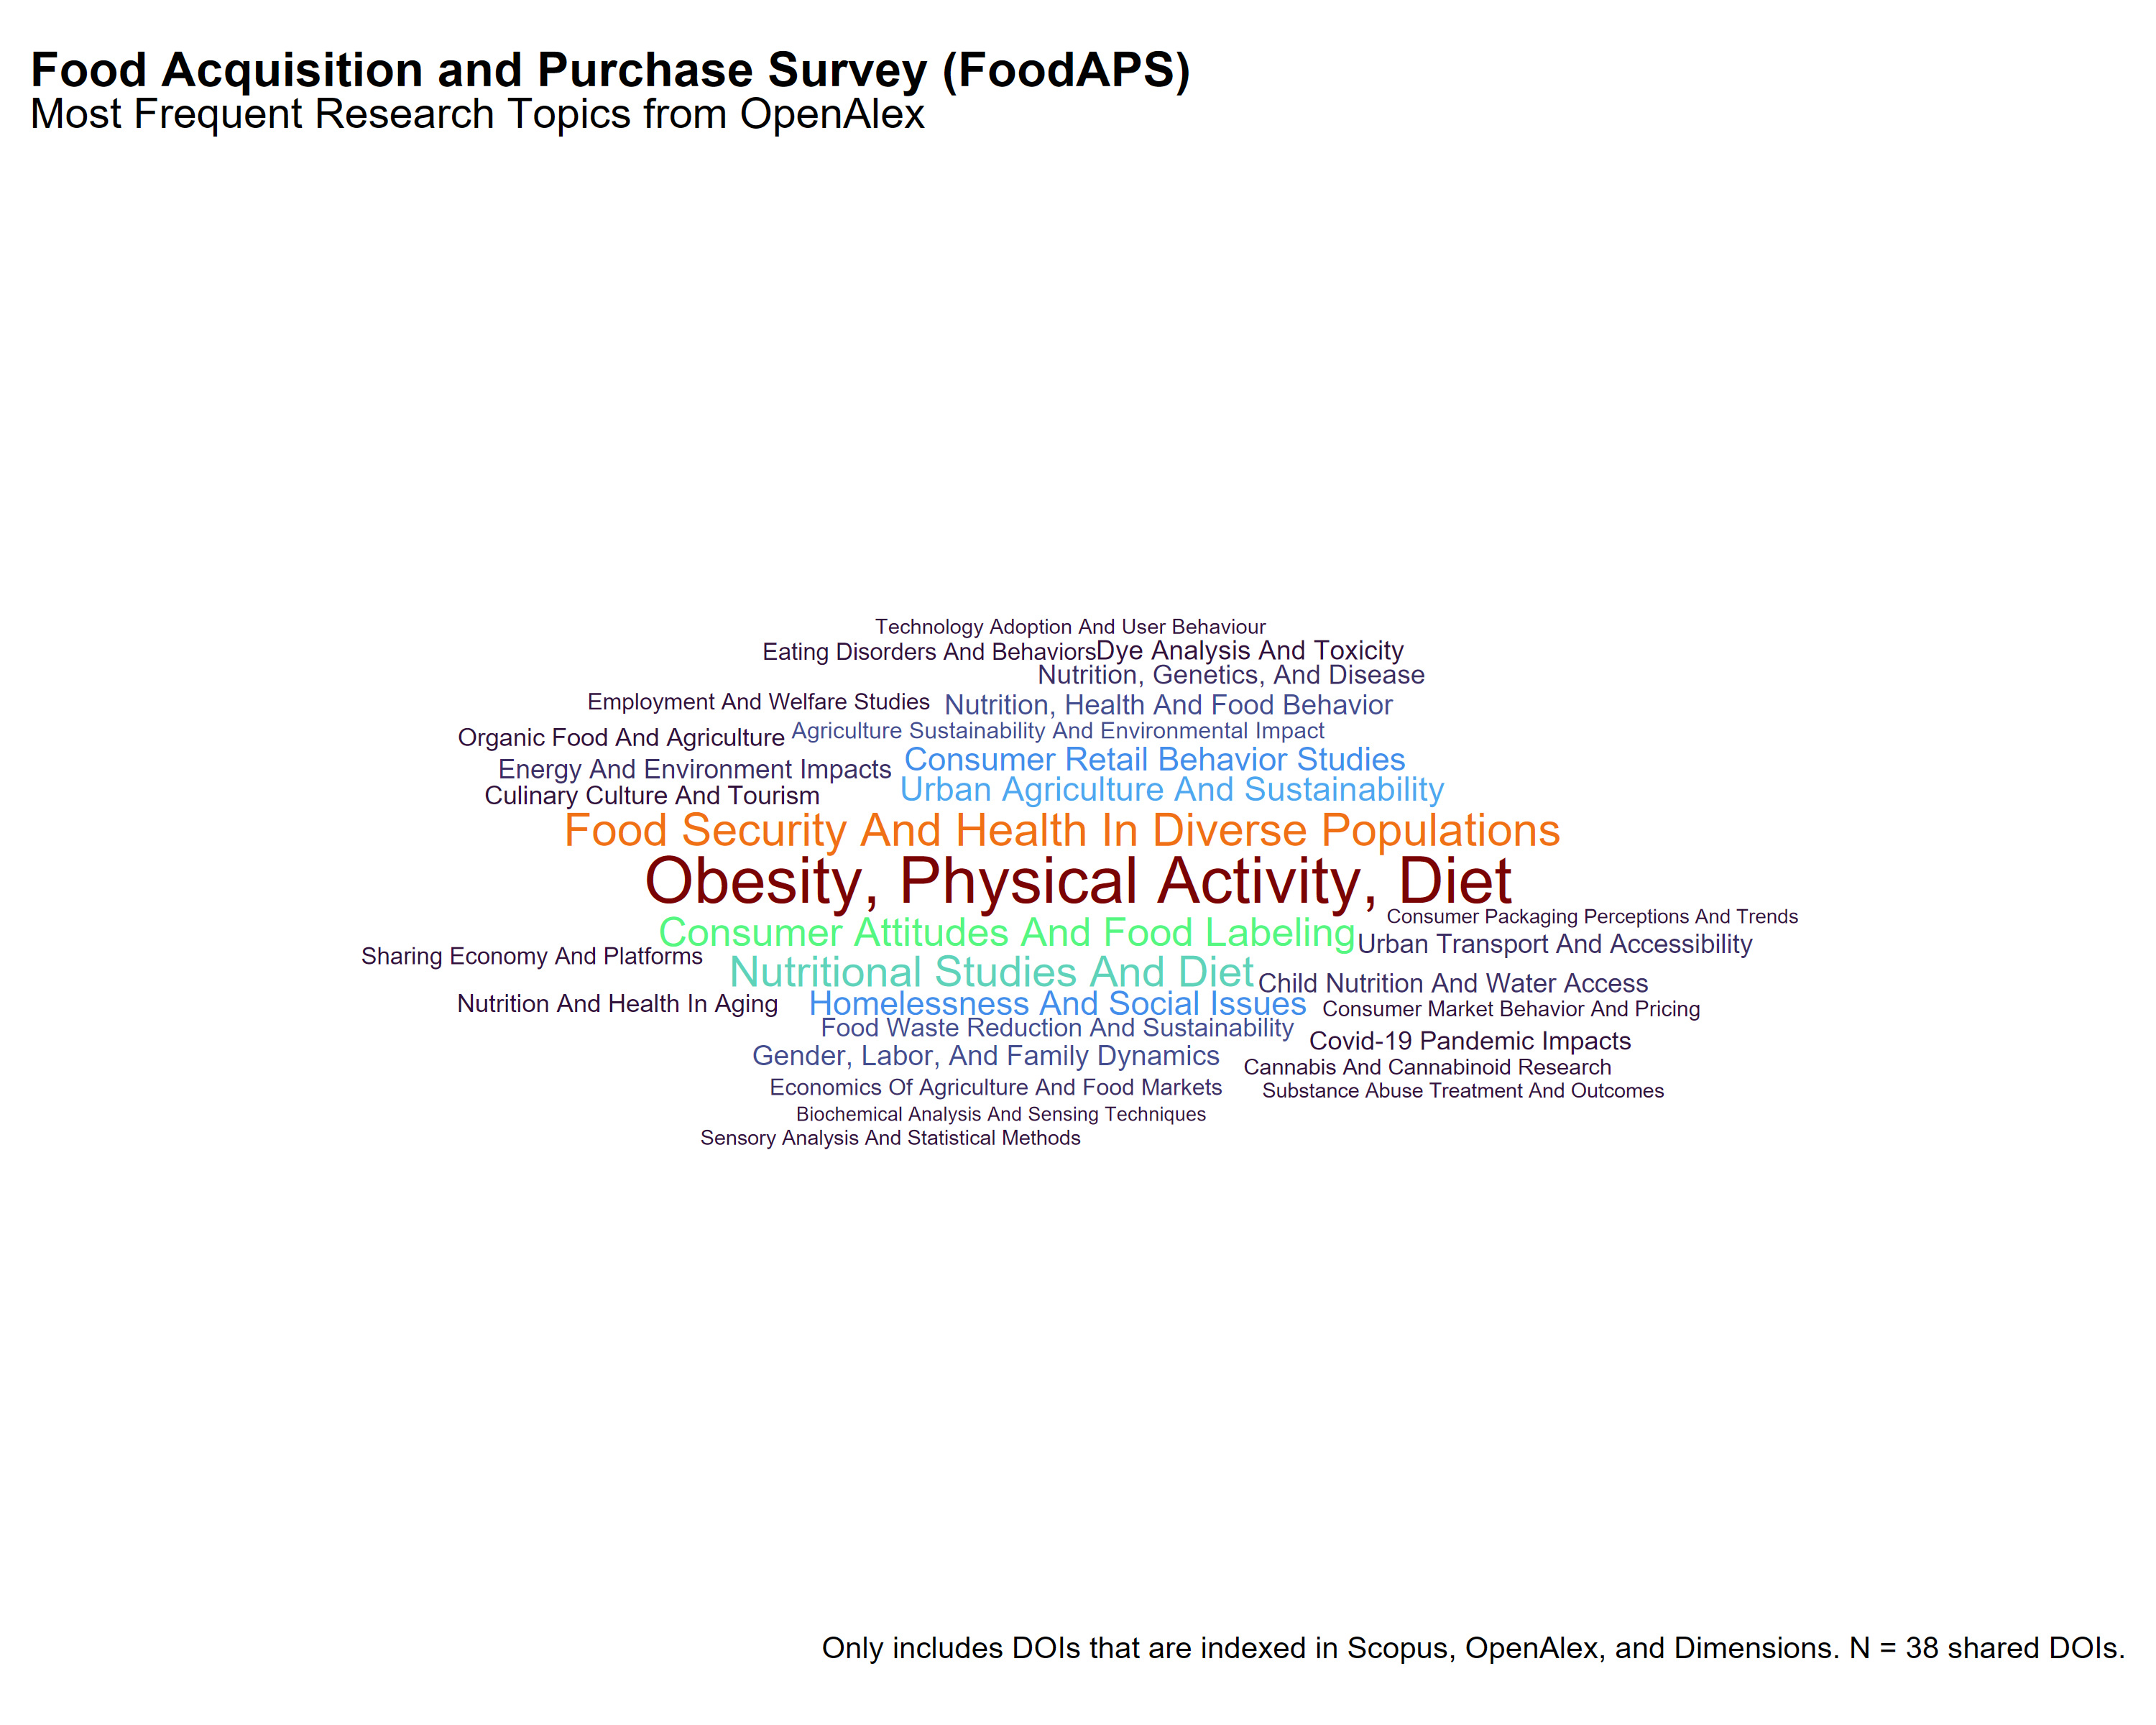
\includegraphics[keepaspectratio]{graphics/word_clouds/shared_dois/dataset09_wordcloud_shared_openalex.png}}

\paragraph{Dimensions}

\pandocbounded{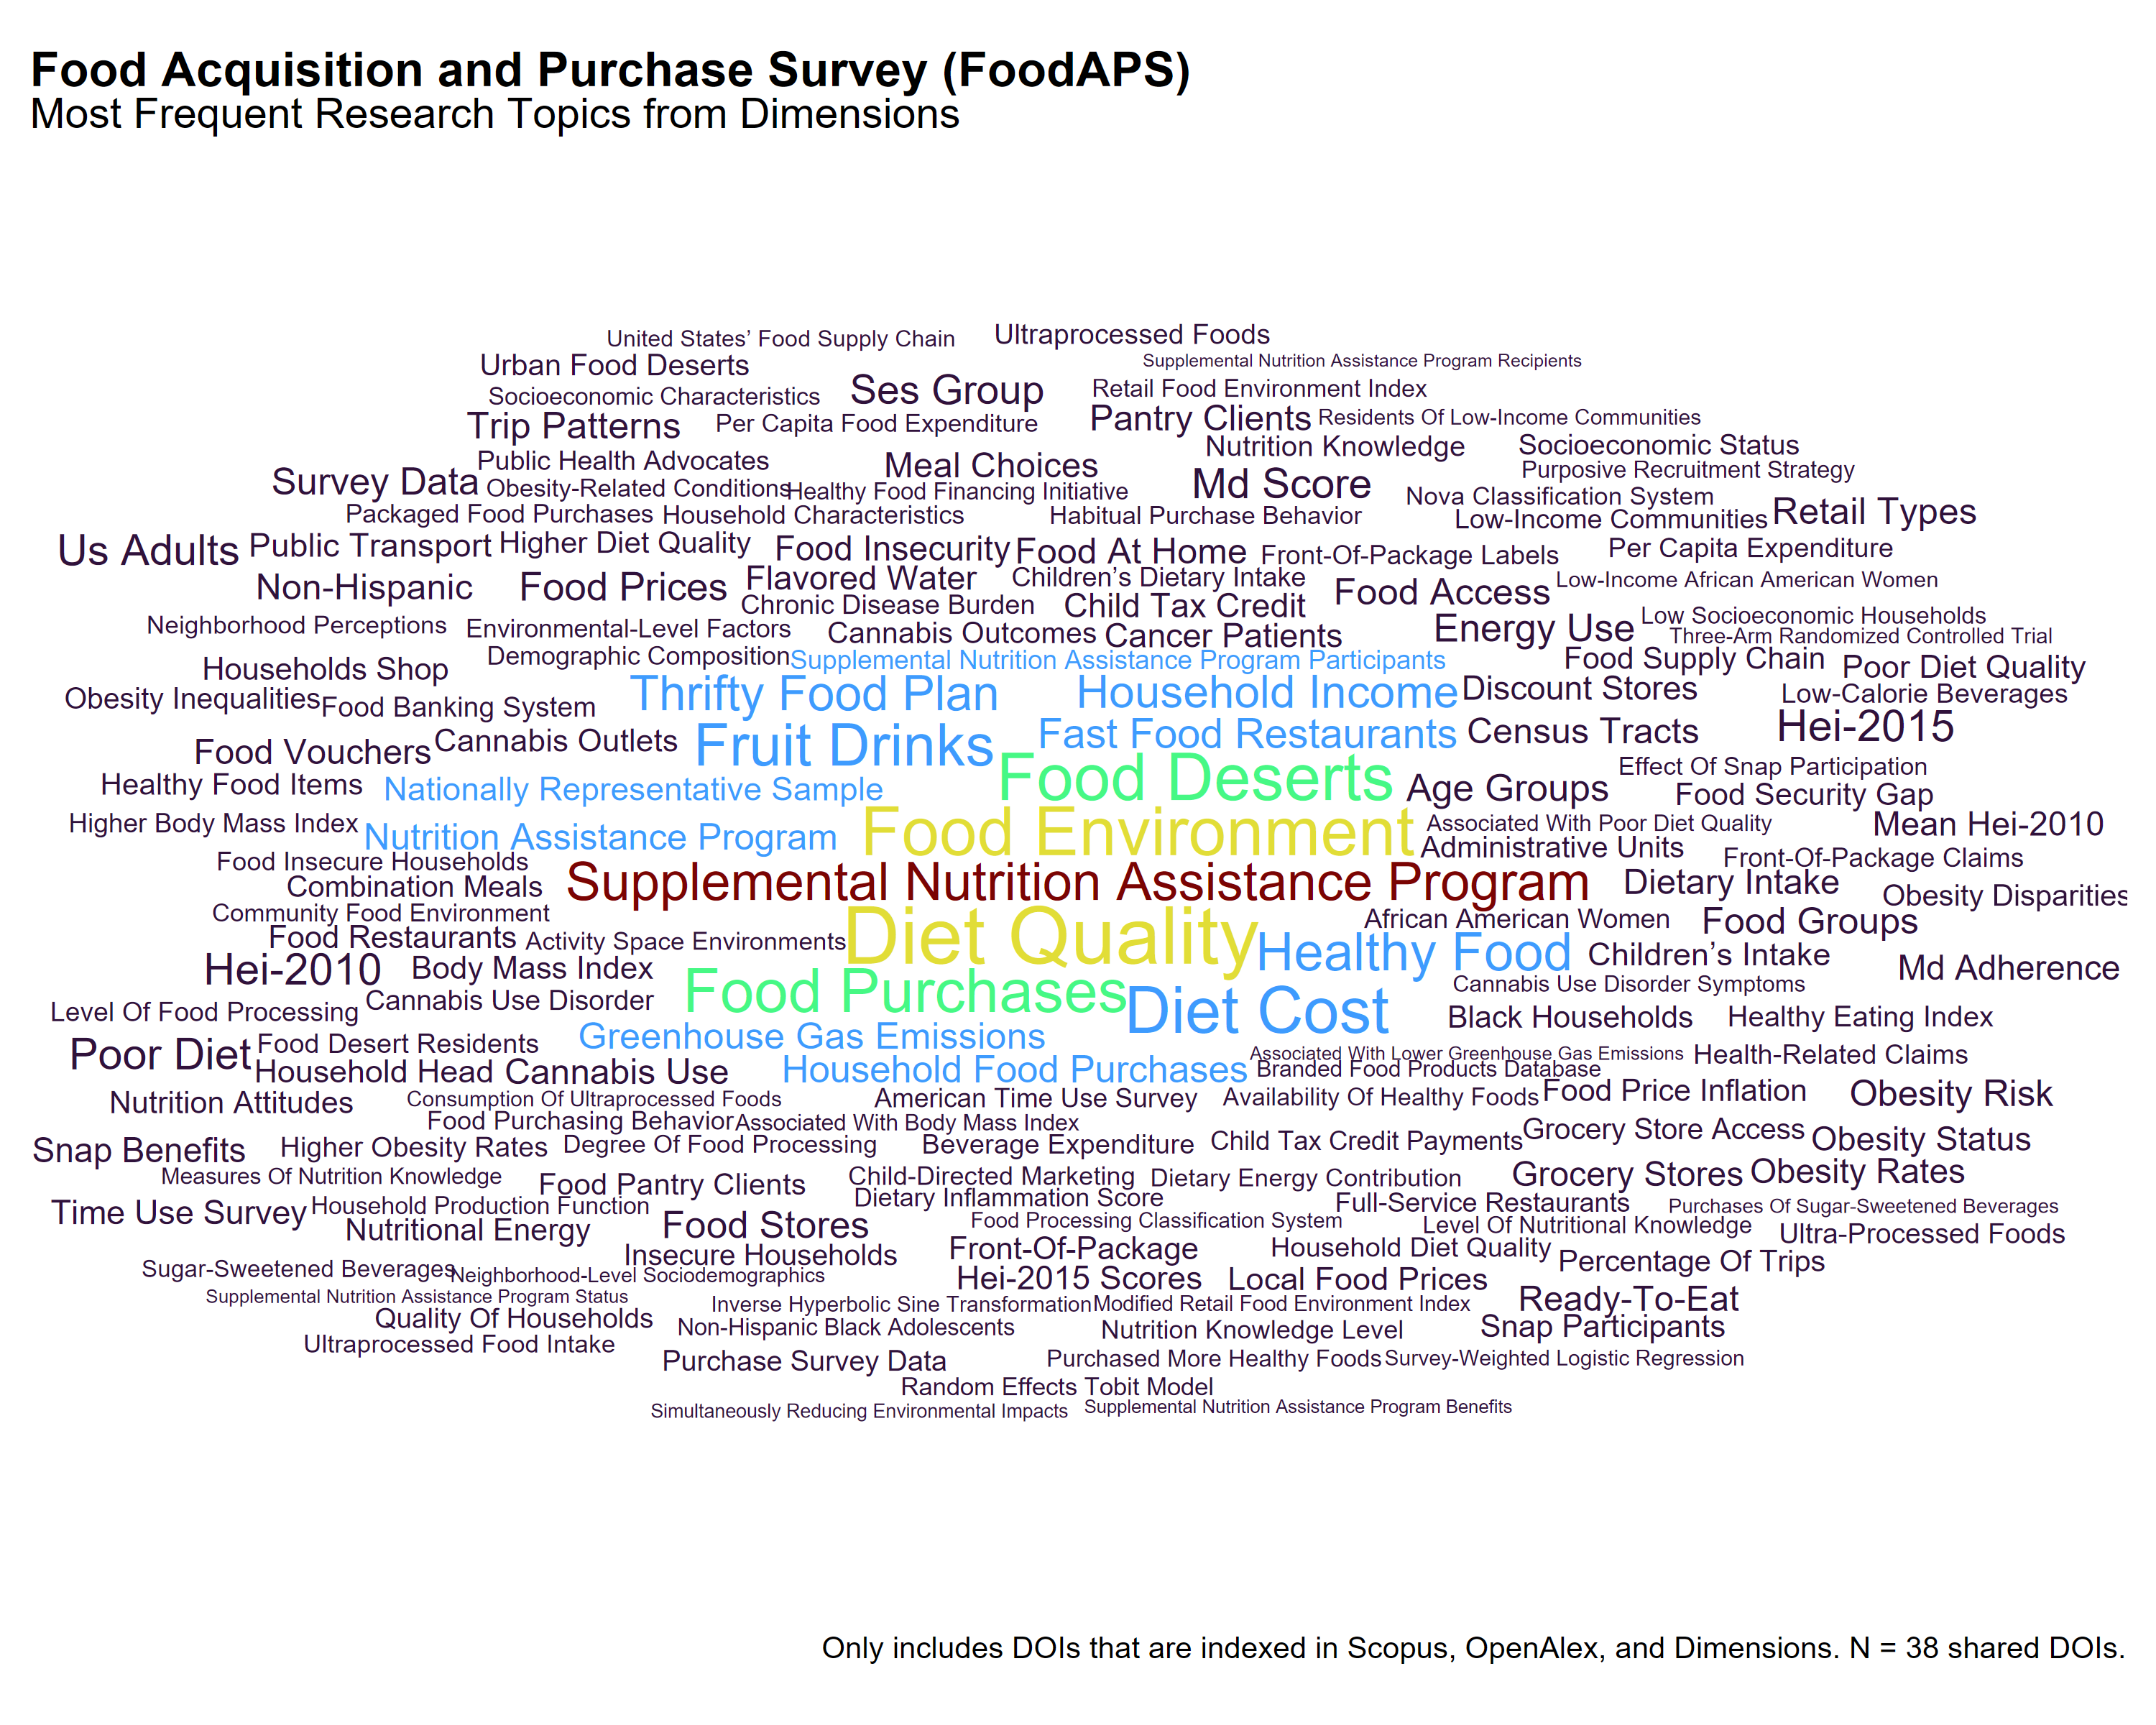
\includegraphics[keepaspectratio]{graphics/word_clouds/shared_dois/dataset09_wordcloud_shared_dimensions.png}}

The next set of word clouds summarizes the most frequent research topics
associated with publications that reference a given dataset, based on
each source's topic classification schema. The first word cloud in each
section aggregates topics across all sources---Scopus, OpenAlex, and
Dimensions---to provide a composite view of the research landscape.
Readers can then click on source-specific word clouds, which reflect the
full corpus of DOIs referencing the dataset within each source. These
differences highlight how each platform categorizes scholarly content
and may inform decisions about dataset visibility and disciplinary
reach.

\begin{tcolorbox}[enhanced jigsaw, leftrule=.75mm, colframe=quarto-callout-note-color-frame, toprule=.15mm, titlerule=0mm, colback=white, rightrule=.15mm, opacityback=0, breakable, bottomtitle=1mm, coltitle=black, colbacktitle=quarto-callout-note-color!10!white, left=2mm, toptitle=1mm, opacitybacktitle=0.6, title=\textcolor{quarto-callout-note-color}{\faInfo}\hspace{0.5em}{Additional Word Cloud Variants}, arc=.35mm, bottomrule=.15mm]

\end{tcolorbox}

\paragraph*{The Household Food Security Survey
Module}\label{the-household-food-security-survey-module-2}
\addcontentsline{toc}{paragraph}{The Household Food Security Survey
Module}

Among the 82 DOIs referencing the Household Food Security Survey Module
(HFSSM) that are indexed in Scopus, OpenAlex, and Dimensions, each
citation database reflects a distinct emphasis in topical
classification.

Dimensions highlights food insecurity, supplemental nutrition
assistance, and diet quality as central themes, along with demographic
and health-related topics such as older adults, physical activity,
mental health, and household income. These reflect a strong policy and
program-oriented lens, focused on vulnerable populations and health
outcomes.

OpenAlex surfaces broader population health and structural themes. Top
topics include Food Security and Health in Diverse Populations, Obesity,
Physical Activity, Diet, and Homelessness and Social Issues. The
emphasis here leans toward sociomedical framing and public health
determinants, especially at the community or systems level.

Scopus features terms like Food Pantries, Program Participation, and
Family Characteristic, consistent with food access research. But it also
brings in more disciplinary and biomedical language---Epigenetics,
Cancer, Autism, and Mindfulness---pointing to research that draws on
HFSSM data to explore clinical and psychological outcomes.

Together, these patterns show how different databases frame the same set
of publications through different classification systems. While the core
themes of food security and health are shared, each source emphasizes
different disciplinary, policy, or structural dimensions of the
research.

\paragraph{Scopus}

\pandocbounded{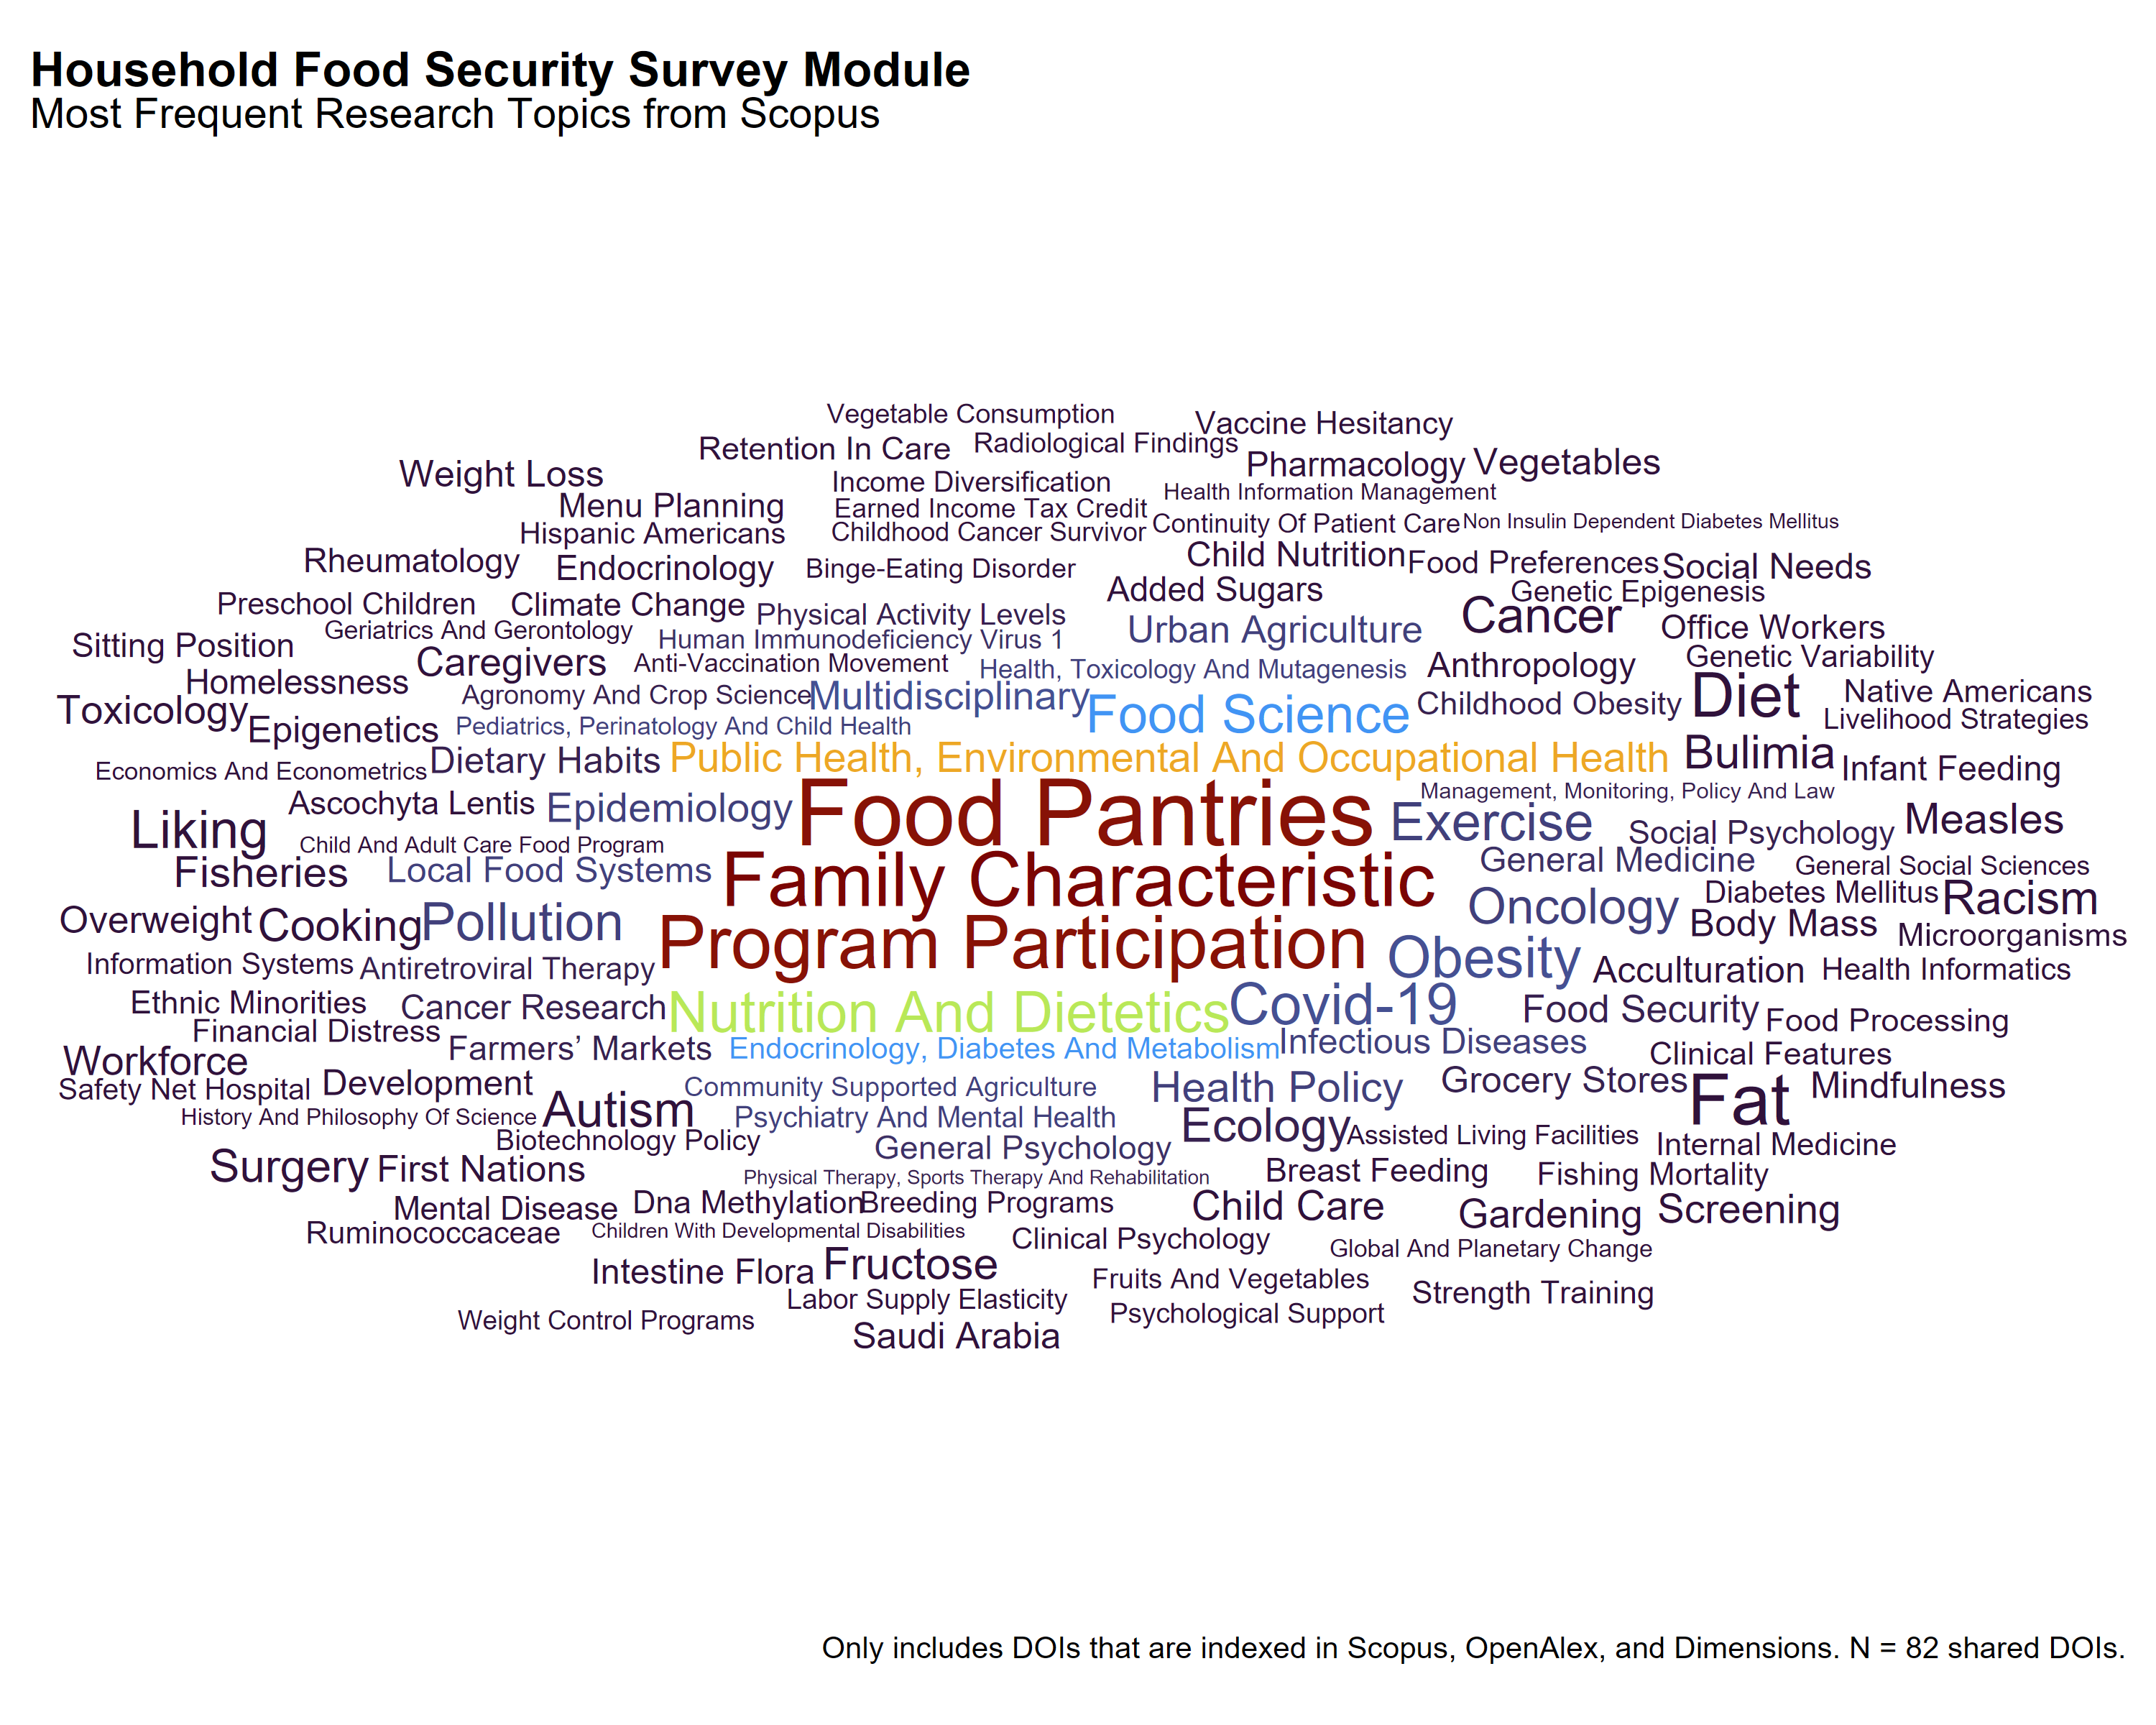
\includegraphics[keepaspectratio]{graphics/word_clouds/shared_dois/dataset10_wordcloud_shared_scopus.png}}

\paragraph{OpenAlex}

\pandocbounded{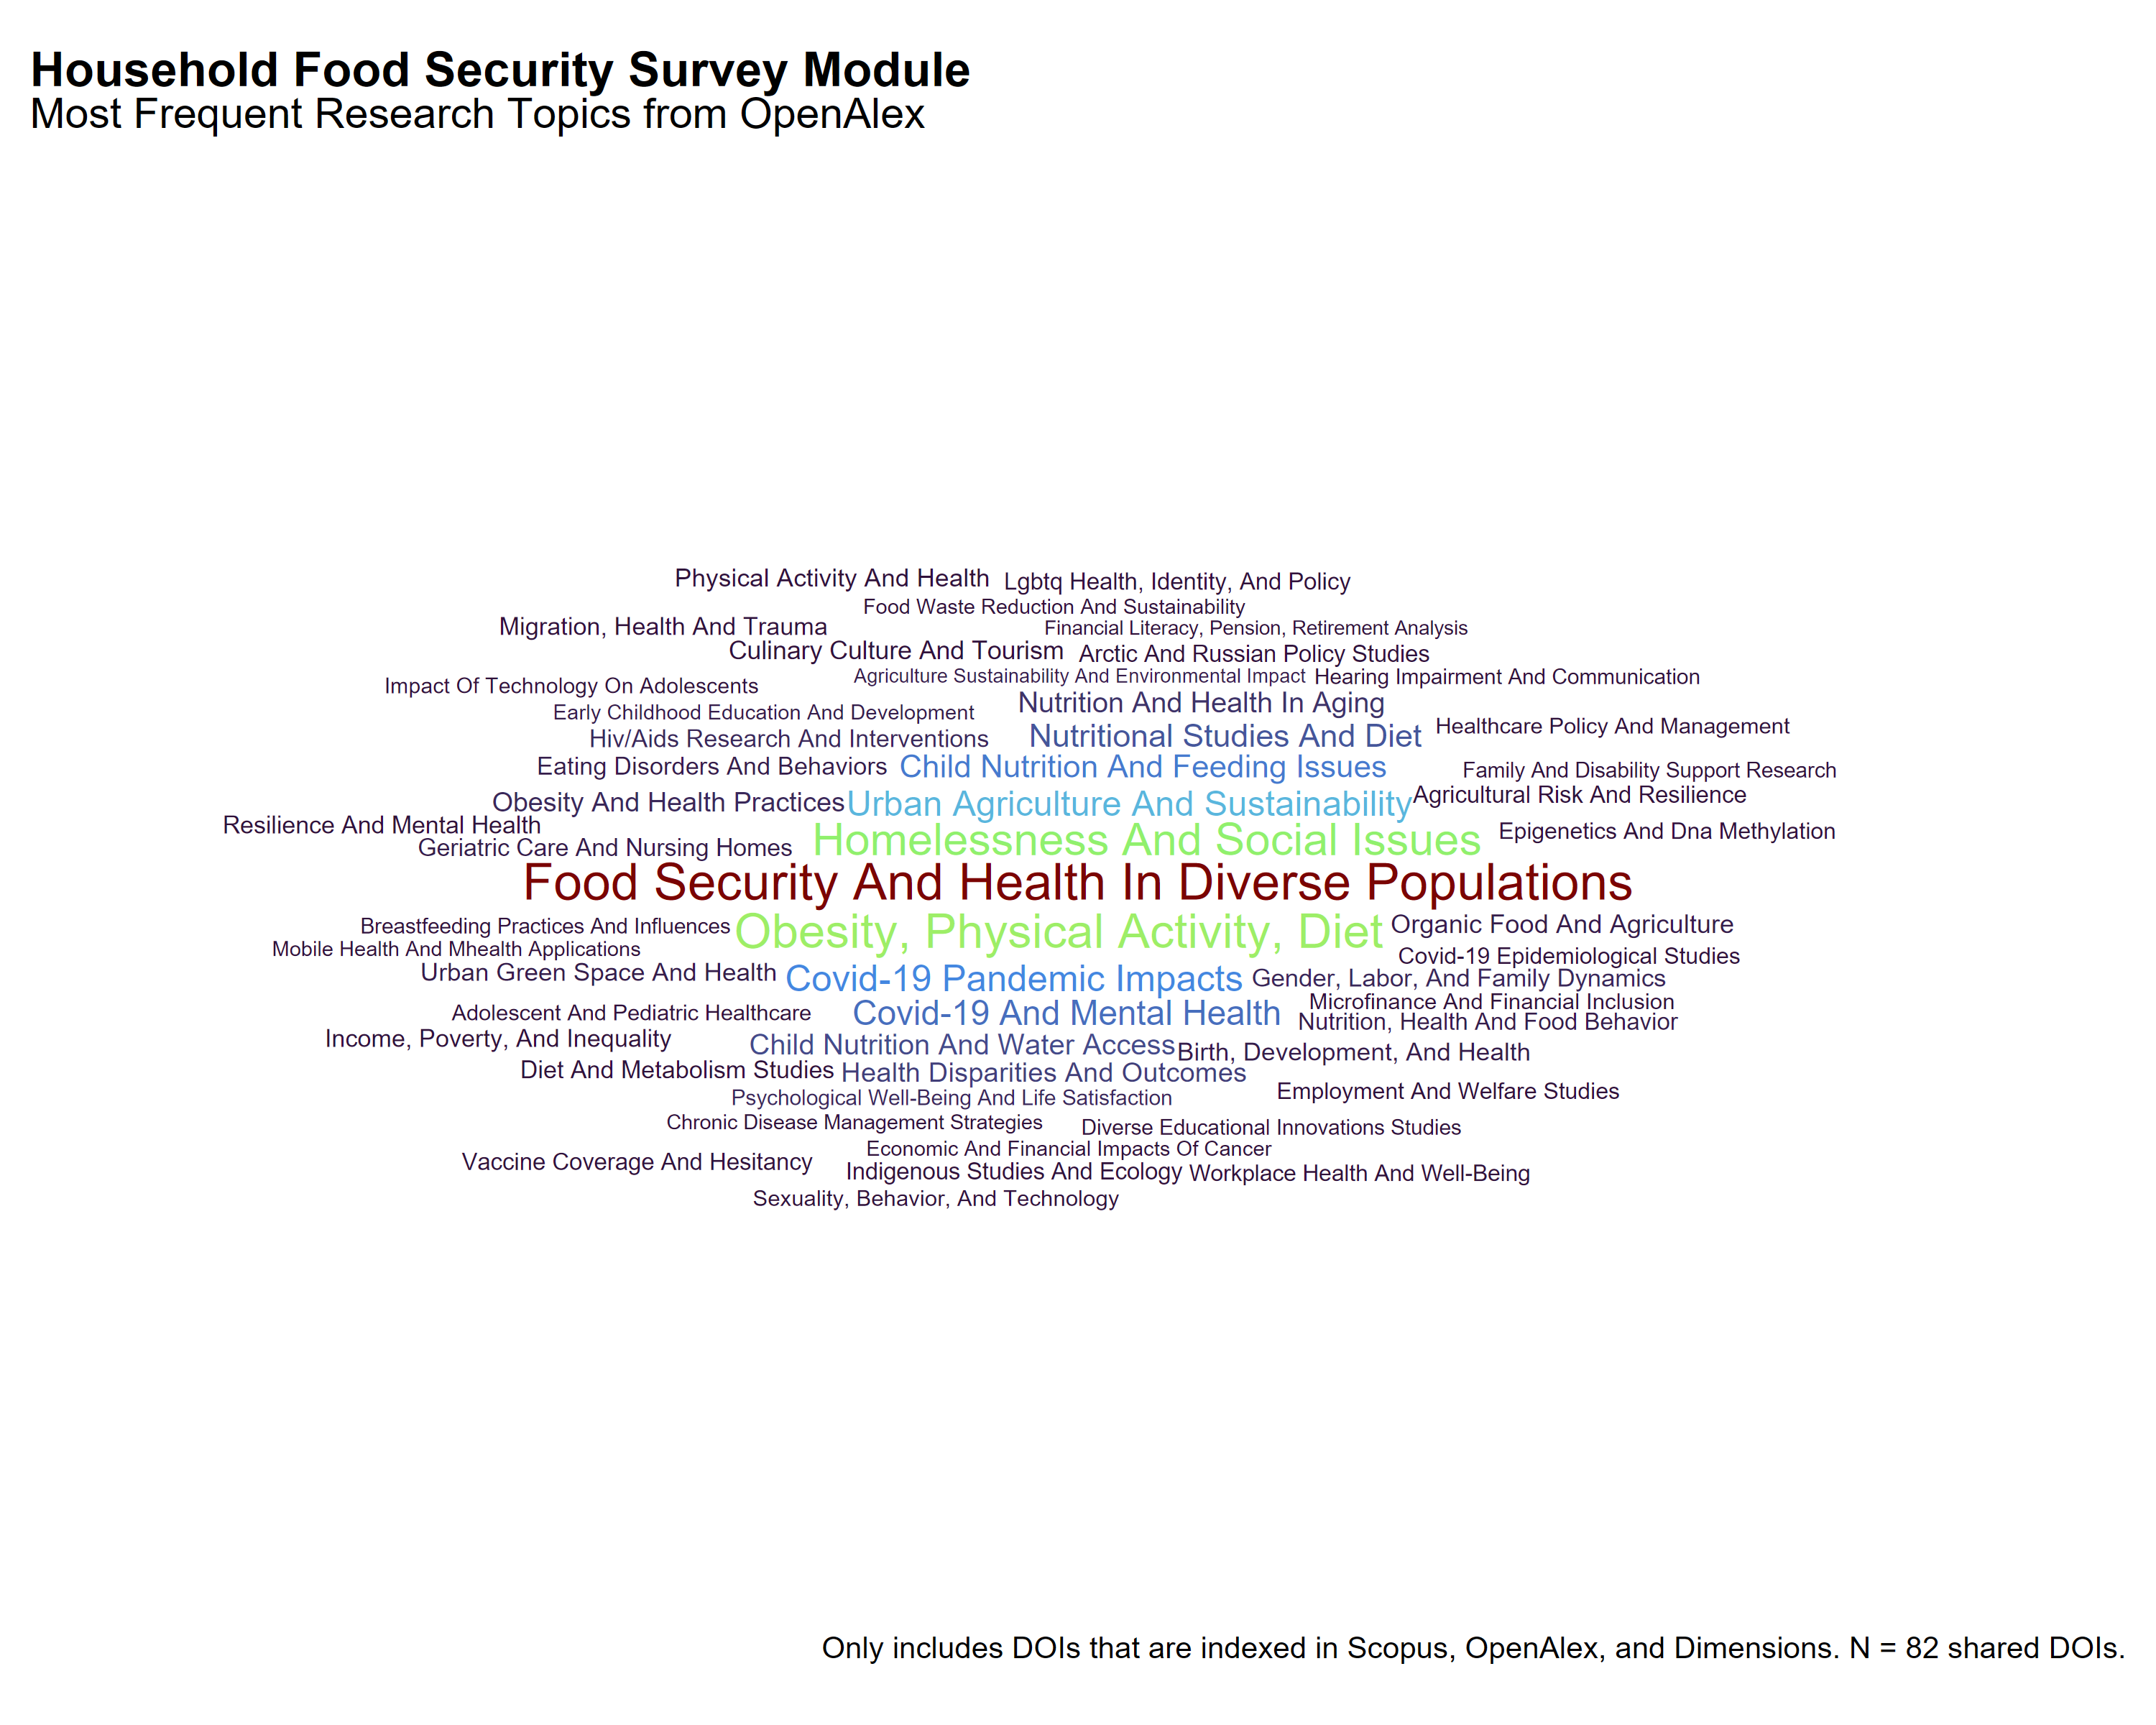
\includegraphics[keepaspectratio]{graphics/word_clouds/shared_dois/dataset10_wordcloud_shared_openalex.png}}

\paragraph{Dimensions}

\pandocbounded{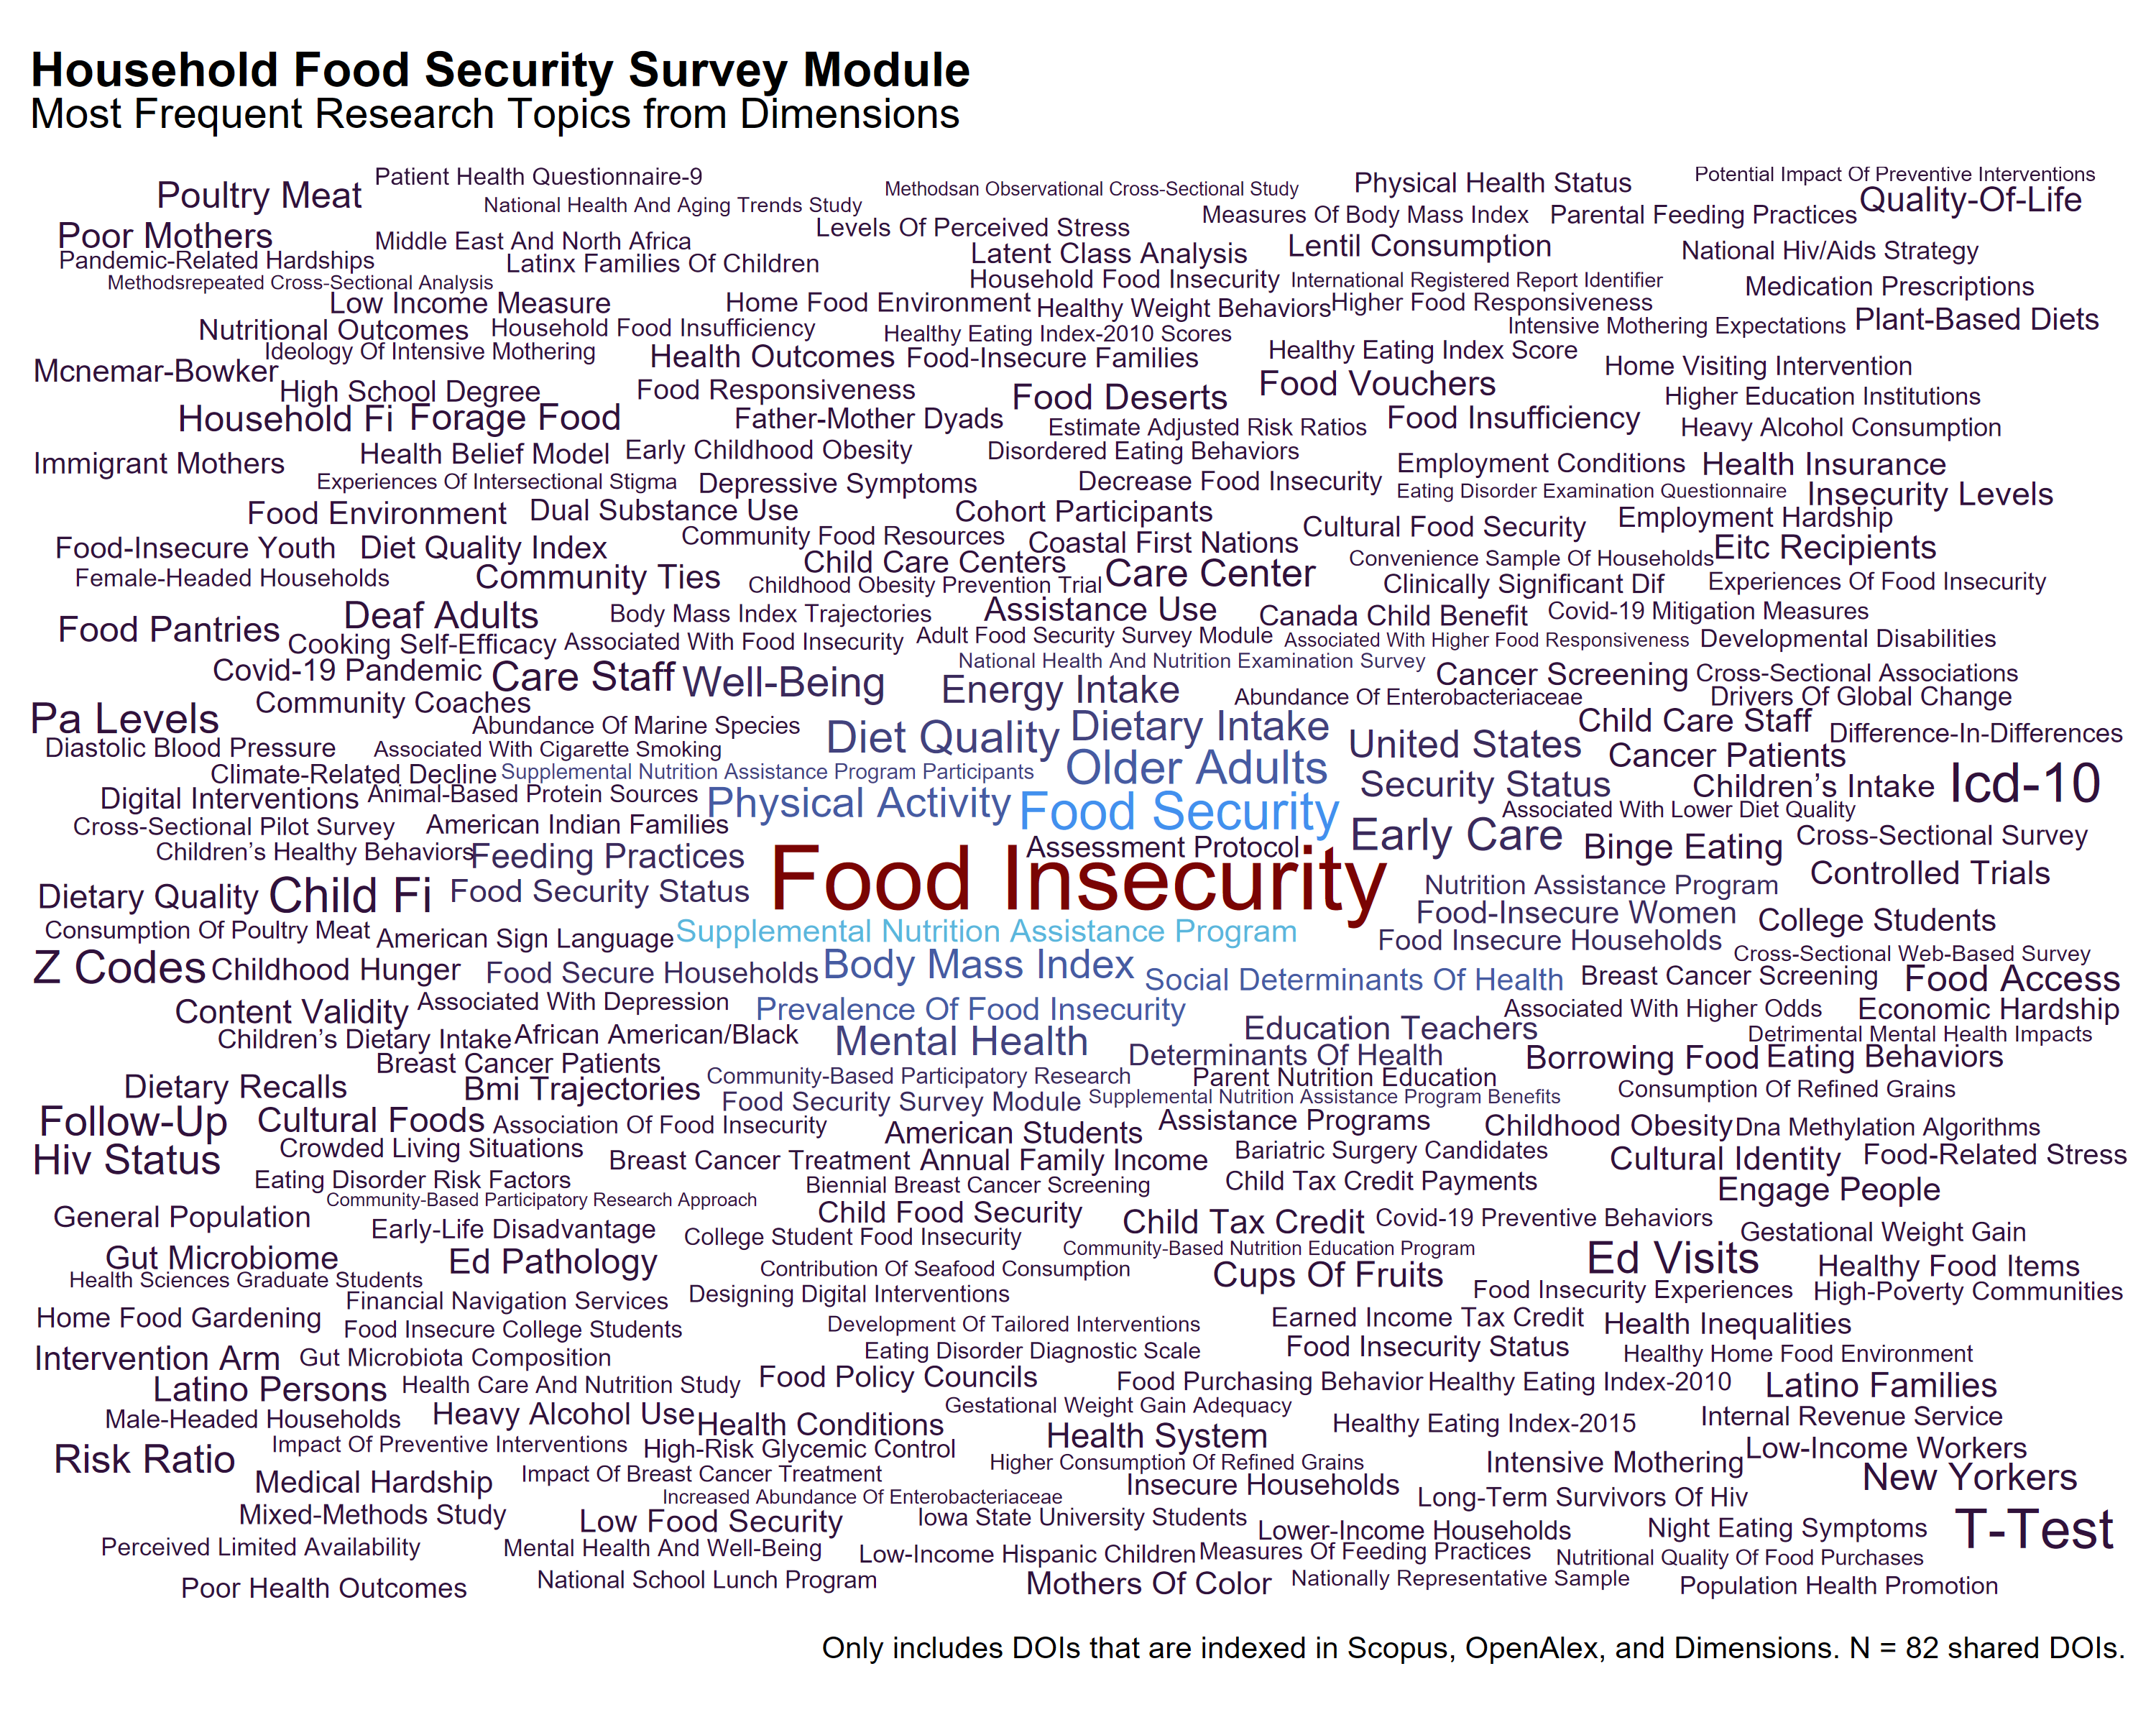
\includegraphics[keepaspectratio]{graphics/word_clouds/shared_dois/dataset10_wordcloud_shared_dimensions.png}}

The next set of word clouds summarizes the most frequent research topics
associated with publications that reference a given dataset, based on
each source's topic classification schema. The first word cloud in each
section aggregates topics across all sources---Scopus, OpenAlex, and
Dimensions---to provide a composite view of the research landscape.
Readers can then click on source-specific word clouds, which reflect the
full corpus of DOIs referencing the dataset within each source. These
differences highlight how each platform categorizes scholarly content
and may inform decisions about dataset visibility and disciplinary
reach.

\begin{tcolorbox}[enhanced jigsaw, leftrule=.75mm, colframe=quarto-callout-note-color-frame, toprule=.15mm, titlerule=0mm, colback=white, rightrule=.15mm, opacityback=0, breakable, bottomtitle=1mm, coltitle=black, colbacktitle=quarto-callout-note-color!10!white, left=2mm, toptitle=1mm, opacitybacktitle=0.6, title=\textcolor{quarto-callout-note-color}{\faInfo}\hspace{0.5em}{Additional Word Cloud Variants}, arc=.35mm, bottomrule=.15mm]

\end{tcolorbox}

\paragraph*{Rural-Urban Continuum
Code}\label{rural-urban-continuum-code-2}
\addcontentsline{toc}{paragraph}{Rural-Urban Continuum Code}

Among the 130 DOIs referencing the Rural-Urban Continuum Code (RUCC)
dataset that appear in Scopus, OpenAlex, and Dimensions, topic
classifications consistently focus on rural health disparities,
healthcare access, and population-level outcomes, though each database
frames these themes differently.

Dimensions places the strongest emphasis on county-level characteristics
and rural infrastructure. Terms such as rural counties, older adults,
cancer incidence, and opioid use disorder are prominent, reflecting the
dataset's utility for examining geographic variation in health outcomes
and healthcare delivery.

OpenAlex centers its taxonomy on population health and structural
factors. Topics like opioid use disorder treatment, health disparities
and outcomes, and global cancer incidence and screening signal a focus
on equity and large-scale health systems research. Behavioral health and
environmental health are also prominent themes.

Scopus reflects a broader mix of clinical and disciplinary topics.
Frequent terms include Covid-19, cancer, public health, obesity, and
health policy. Additional tags such as smoking ban, rural poverty, and
Medicaid point to both policy-oriented and biomedical lines of research.

Together, these differences illustrate how the same publications are
categorized through different topical lenses, depending on the
underlying classification systems used by each database.

\paragraph{Scopus}

\pandocbounded{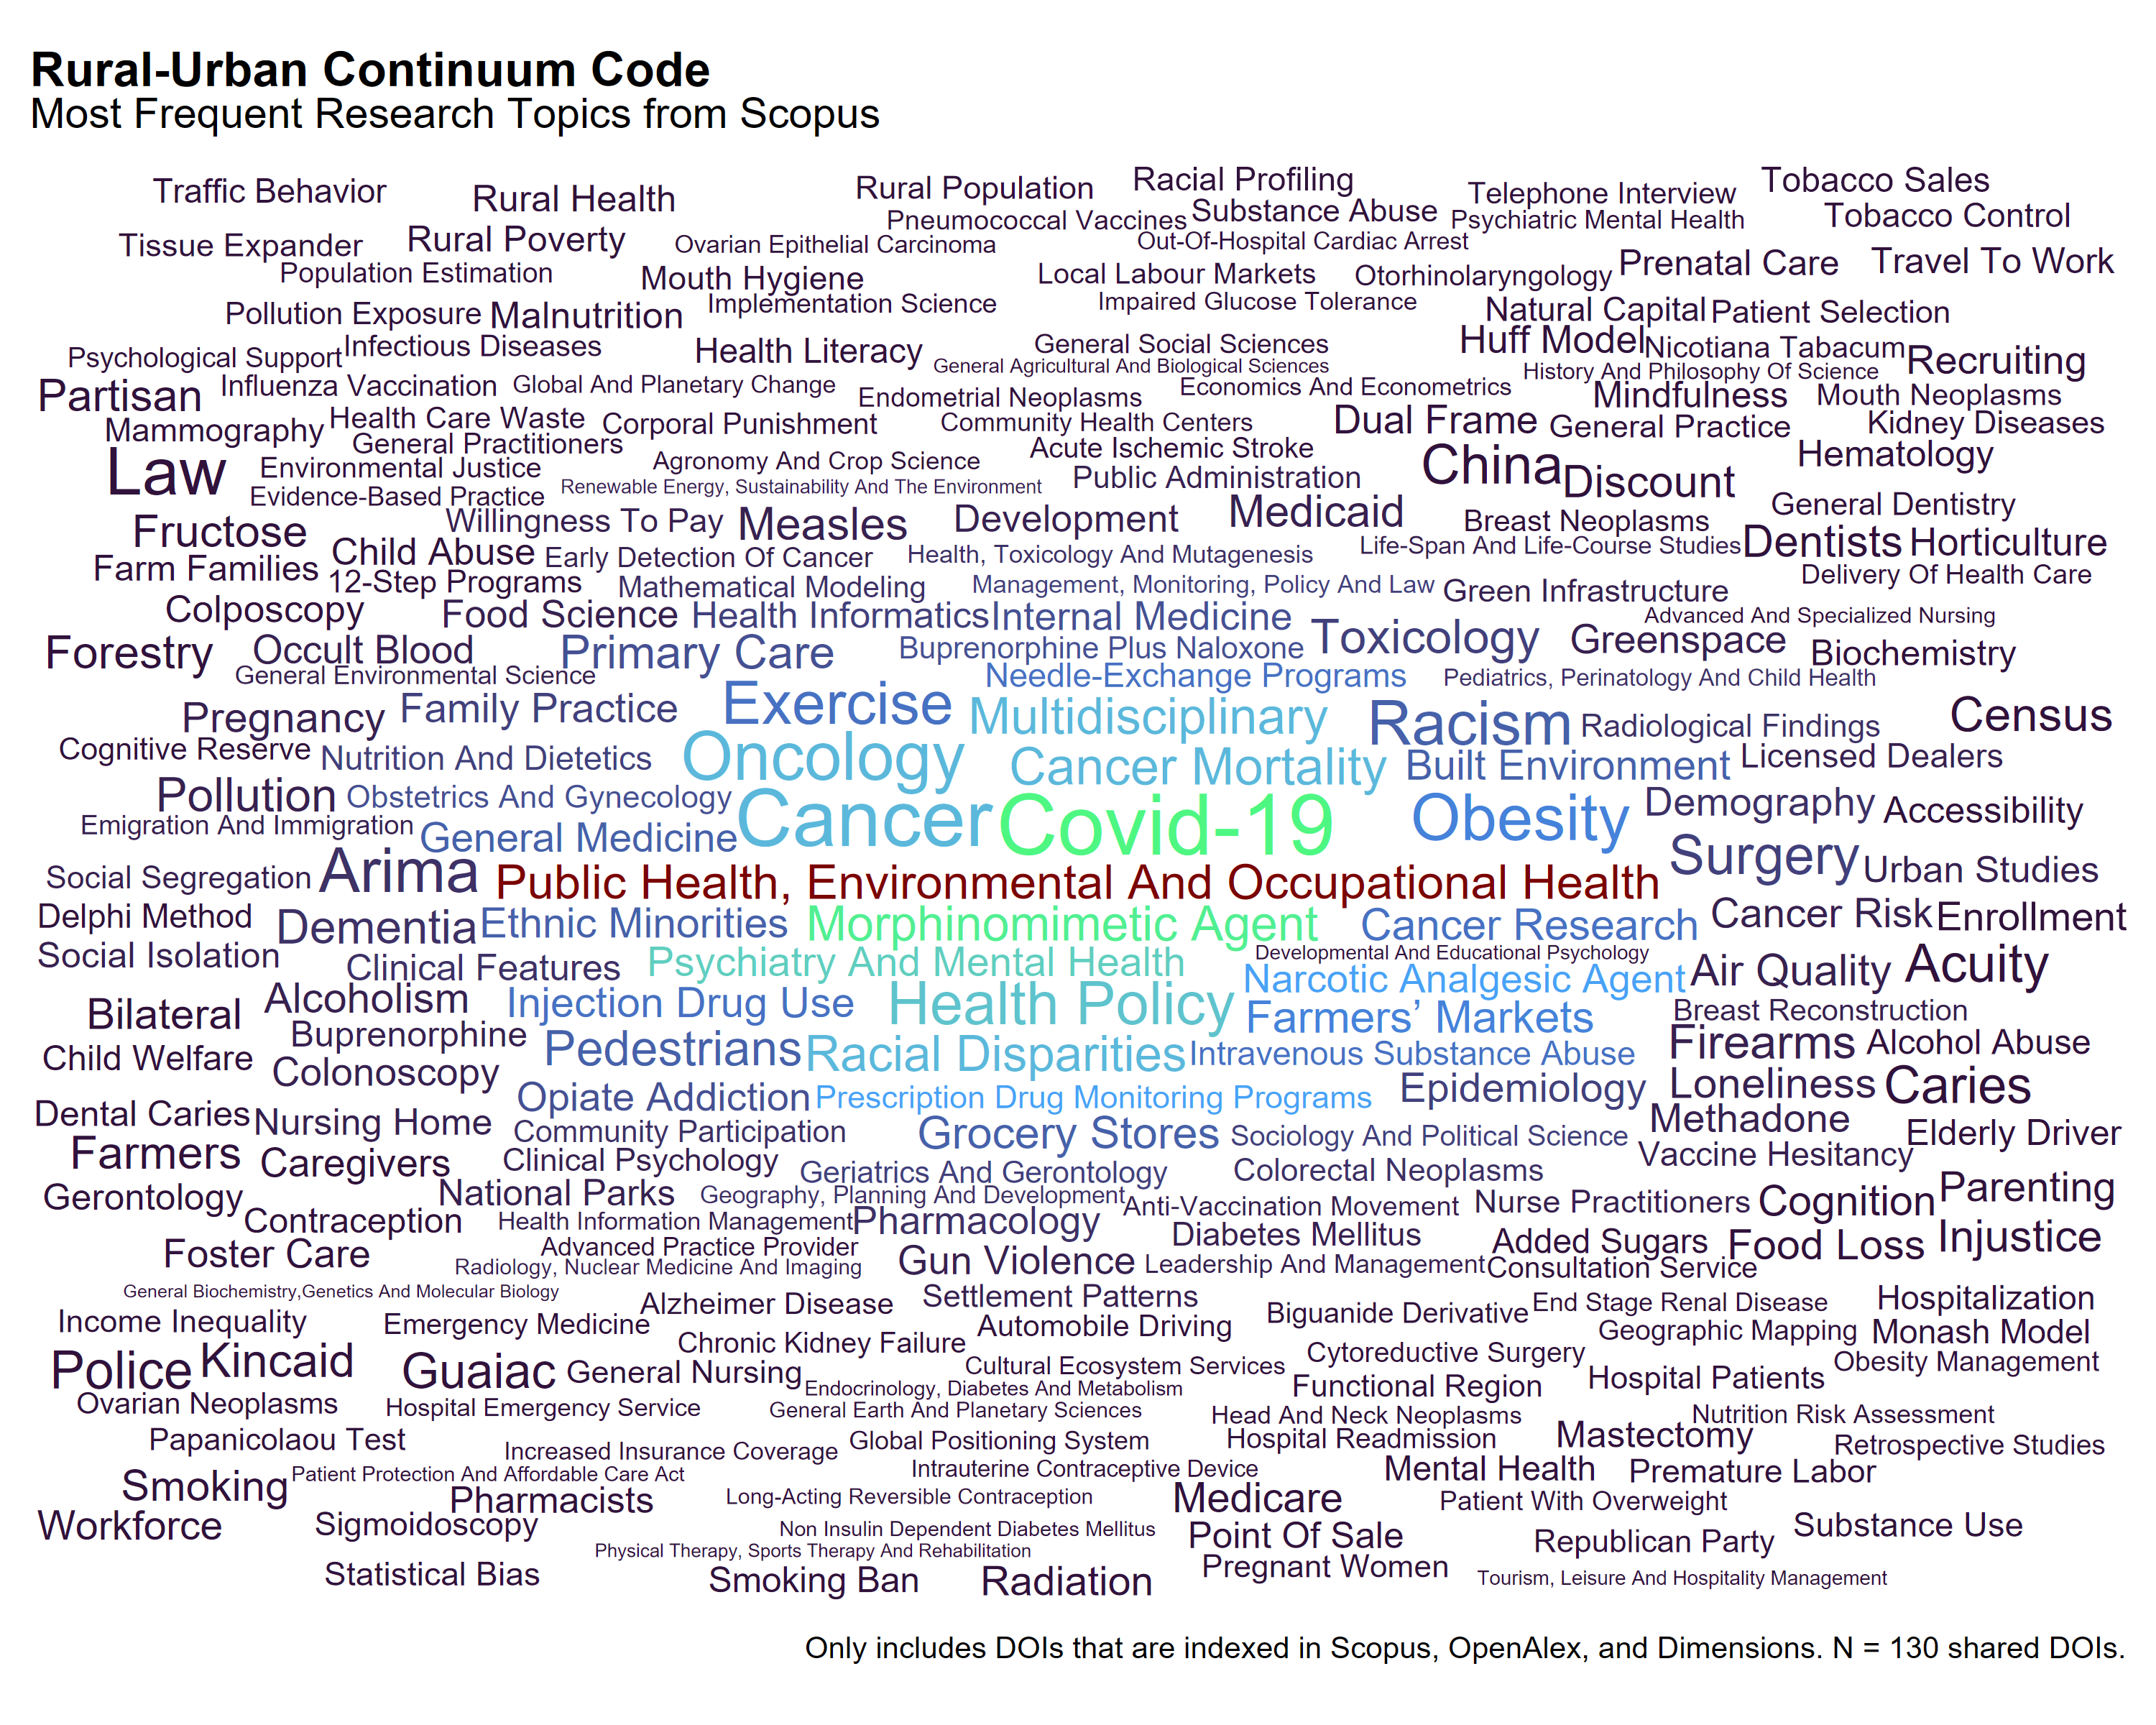
\includegraphics[keepaspectratio]{graphics/word_clouds/shared_dois/dataset06_wordcloud_shared_scopus.png}}

\paragraph{OpenAlex}

\pandocbounded{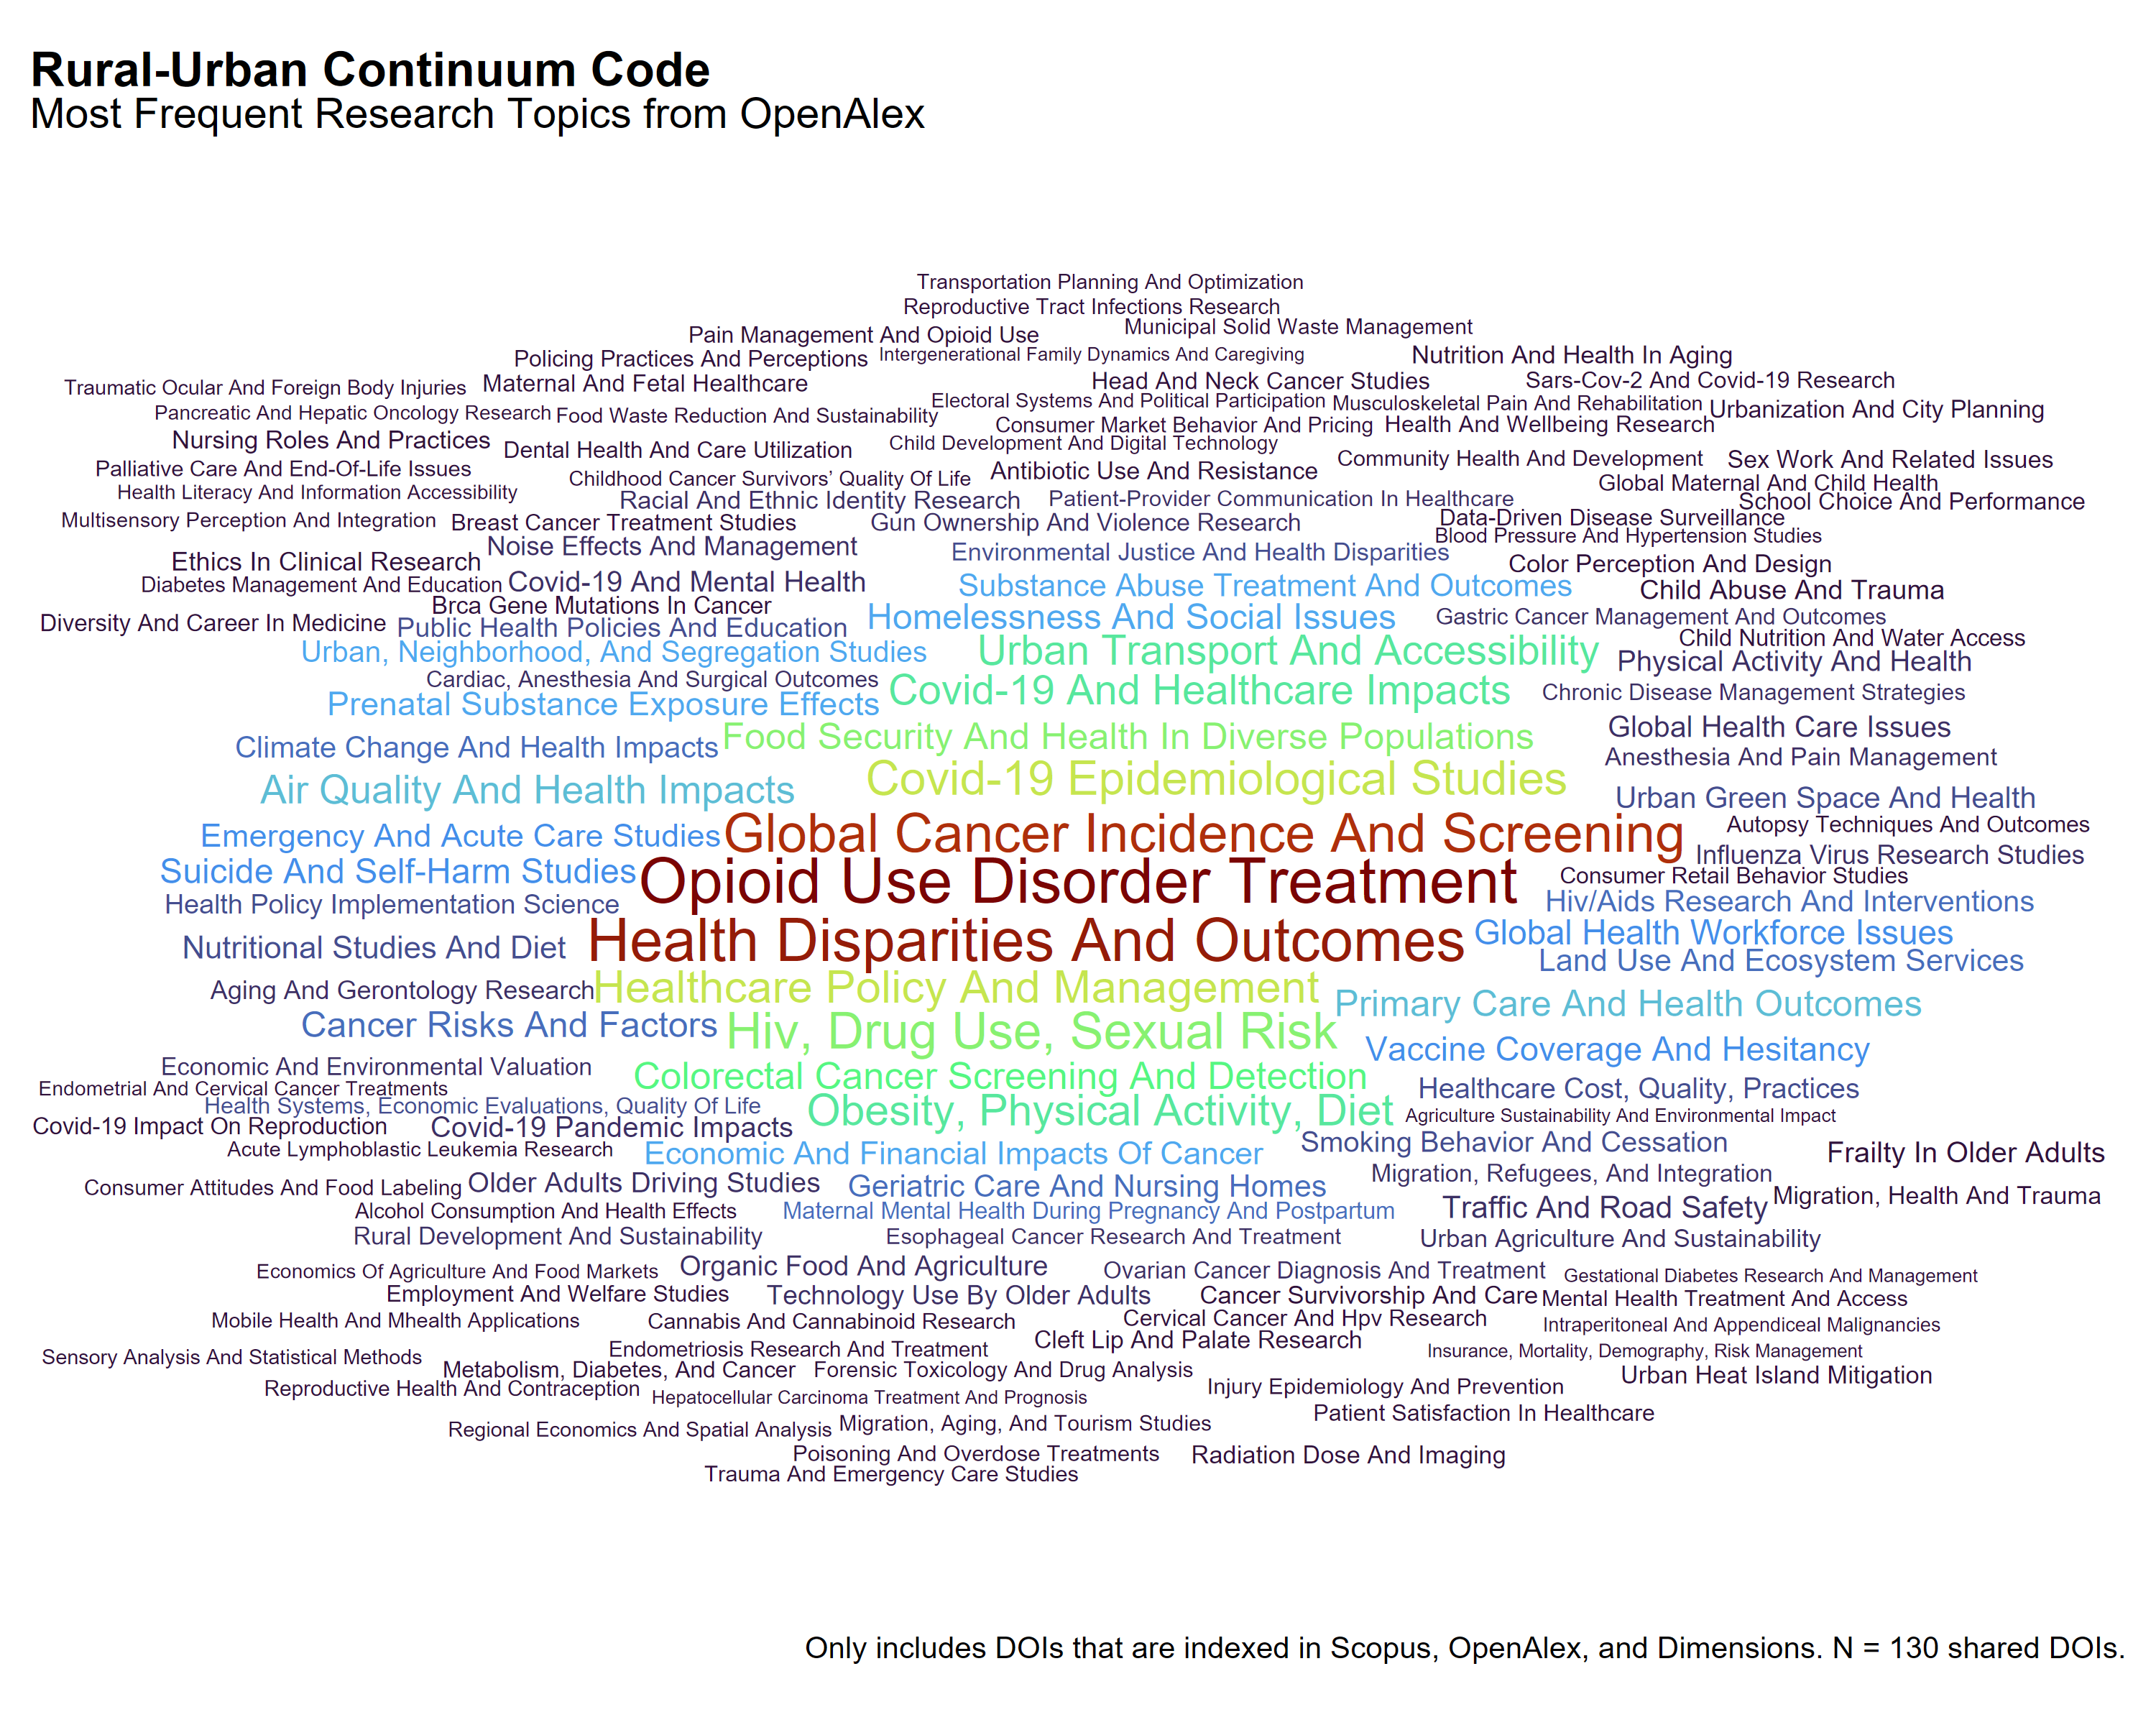
\includegraphics[keepaspectratio]{graphics/word_clouds/shared_dois/dataset06_wordcloud_shared_openalex.png}}

\paragraph{Dimensions}

\pandocbounded{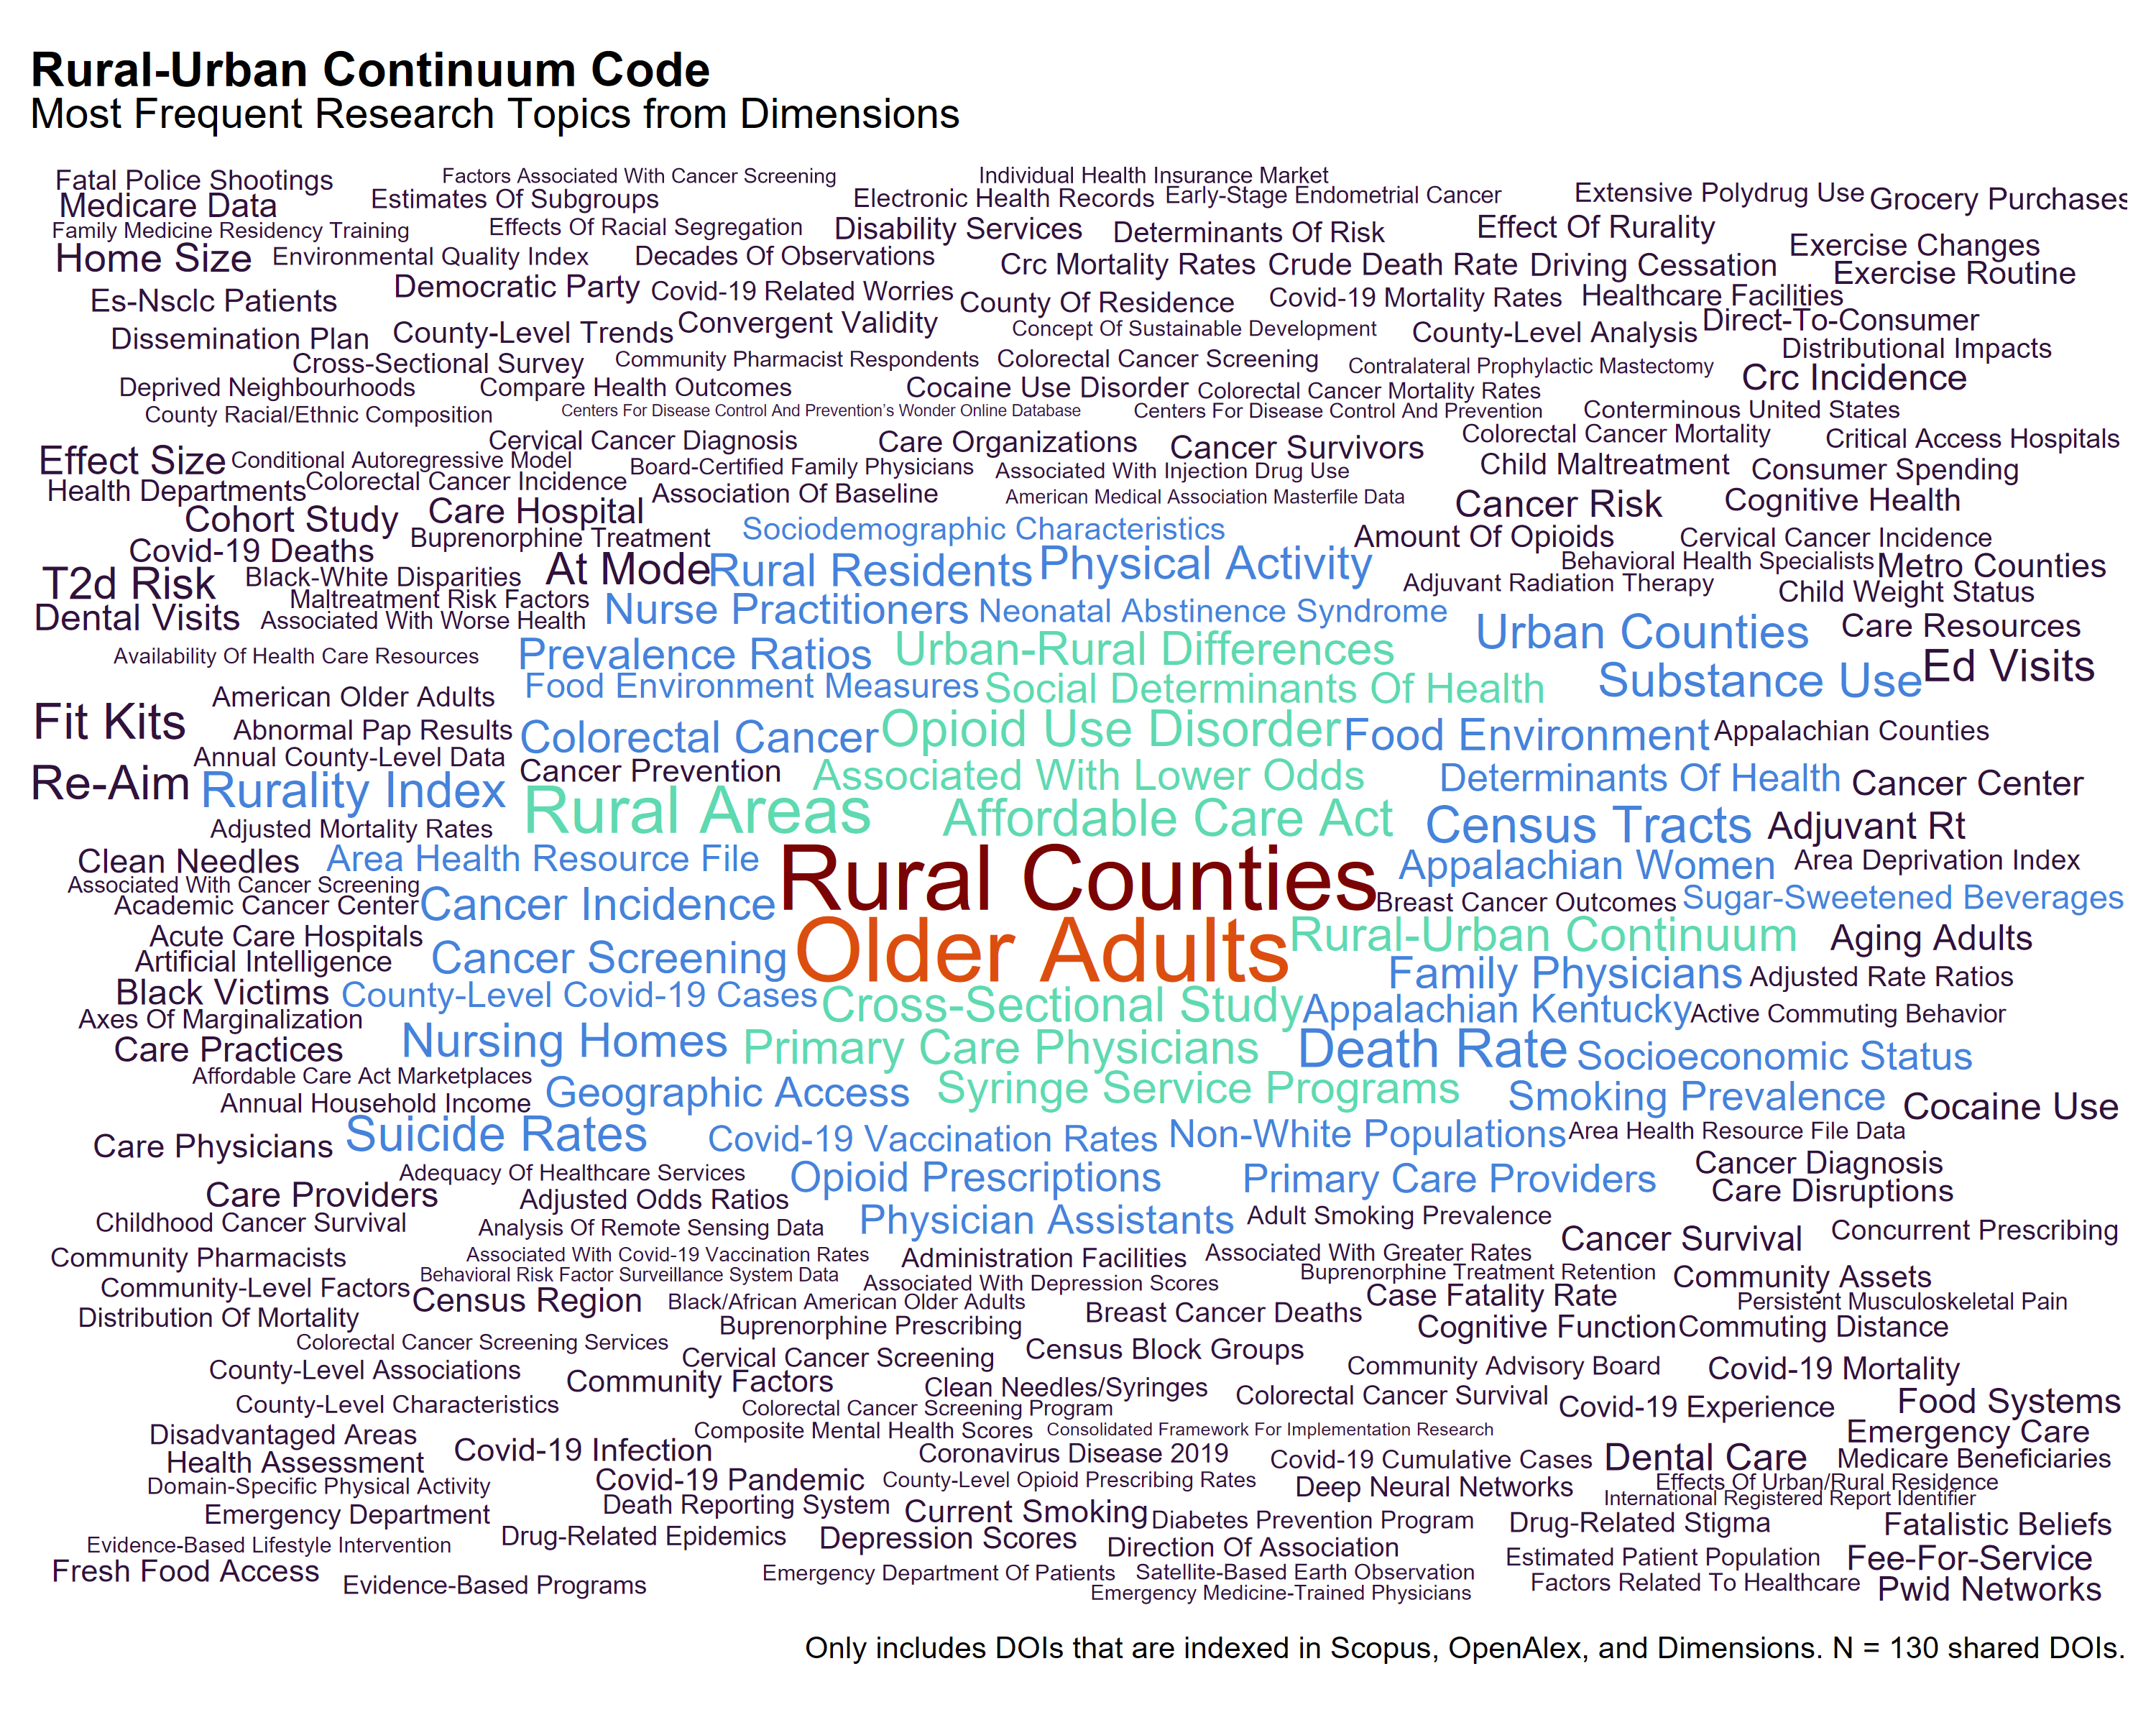
\includegraphics[keepaspectratio]{graphics/word_clouds/shared_dois/dataset06_wordcloud_shared_dimensions.png}}

The next set of word clouds summarizes the most frequent research topics
associated with publications that reference a given dataset, based on
each source's topic classification schema. The first word cloud in each
section aggregates topics across all sources---Scopus, OpenAlex, and
Dimensions---to provide a composite view of the research landscape.
Readers can then click on source-specific word clouds, which reflect the
full corpus of DOIs referencing the dataset within each source. These
differences highlight how each platform categorizes scholarly content
and may inform decisions about dataset visibility and disciplinary
reach.

\begin{tcolorbox}[enhanced jigsaw, leftrule=.75mm, colframe=quarto-callout-note-color-frame, toprule=.15mm, titlerule=0mm, colback=white, rightrule=.15mm, opacityback=0, breakable, bottomtitle=1mm, coltitle=black, colbacktitle=quarto-callout-note-color!10!white, left=2mm, toptitle=1mm, opacitybacktitle=0.6, title=\textcolor{quarto-callout-note-color}{\faInfo}\hspace{0.5em}{Additional Word Cloud Variants}, arc=.35mm, bottomrule=.15mm]

\end{tcolorbox}

\subsubsection{Author Comparison}\label{author-comparison}

To identify and compare authors across Scopus, OpenAlex, and Dimensions,
a multi-step disambiguation process was implemented. Because not all
authors have persistent identifiers (e.g., ORCIDs), and because name
formatting, use of initials, and institutional affiliations vary across
and within sources, a harmonization pipeline was developed. This process
follows the structure of the
\href{https://patentsview.org/disambiguation}{PatentsView disambiguation
methodology} and includes the following steps:

\begin{enumerate}
\def\labelenumi{\arabic{enumi}.}
\item
  \textbf{Name Normalization and Source-Specific Cleaning:} Author names
  were extracted from each source and cleaned using a consistent
  normalization function. This involved transliterating special
  characters, removing punctuation, standardizing case, and collapsing
  whitespace. In each database, author records were linked to
  publication DOIs and enriched with affiliation information where
  available.
\item
  \textbf{ORCID-Based Canonical Resolution:} When an author's ORCID was
  present---either directly in OpenAlex or indirectly via
  Dimensions---it was used as the canonical identifier. ORCID lookups
  were performed for all DOIs across sources, and a lookup table was
  constructed to resolve shared authors using both ORCID and cleaned
  name/DOI matches.
\item
  \textbf{Blocking Using Canopy Construction:} For authors without ORCID
  identifiers, blocking keys were constructed by combining the first
  initial and last name to form ``canopy'' groups. This reduced the
  number of pairwise comparisons needed for clustering by limiting them
  to plausible matches.
\item
  \textbf{String Similarity Clustering Within Canopies:} Within each
  canopy group, Jaro-Winkler string distances were calculated using the
  cleaned full names. Hierarchical clustering with average linkage was
  applied, and clusters were formed using a similarity threshold. Each
  cluster was then assigned a synthetic canonical ID based on the first
  observed name.
\item
  \textbf{Merging and Source Propagation:} Author mentions across all
  three sources were merged into a master long-format table, with
  canonical IDs assigned based on ORCID or string-based clustering. For
  each publication, flags were added to indicate whether an author
  appeared in Scopus, OpenAlex, or Dimensions. These flags were
  propagated to all mentions of a given author within the same DOI.
\item
  \textbf{Institutional Consolidation:} Author affiliations were
  collapsed across sources by pivoting to a wide format (institution\_1,
  institution\_2, etc.) and summarizing into a primary institution
  field. This structure supported subsequent author-level aggregation
  and topic classification.
\end{enumerate}

This approach enables the identification of unique authors across
bibliometric systems, even in the absence of persistent identifiers. It
supports comparisons of author counts, top contributors, and
topic-specific participation across Scopus, OpenAlex, and Dimensions.

\textbf{Main Takeaway}

Across all datasets, the authors most visible in one platform are not
always discoverable in others. The top contributors to a dataset can
vary significantly depending on which citation database is used. These
differences stem from inconsistencies in metadata, name disambiguation,
and indexing practices. As a result, evaluations or dashboards based on
a single source may misrepresent who is using a dataset, leading to
undercounting or omission of active researchers. Using multiple sources
helps create a more accurate and equitable picture of scholarly
engagement.

\subsubsection{Author Mentions by Dataset and Citation Database
(2017--2023, Article-Type
Only)}\label{author-mentions-by-dataset-and-citation-database-20172023-article-type-only}

\begin{longtable}[]{@{}
  >{\raggedright\arraybackslash}p{(\linewidth - 6\tabcolsep) * \real{0.3386}}
  >{\raggedright\arraybackslash}p{(\linewidth - 6\tabcolsep) * \real{0.2047}}
  >{\raggedright\arraybackslash}p{(\linewidth - 6\tabcolsep) * \real{0.2205}}
  >{\raggedright\arraybackslash}p{(\linewidth - 6\tabcolsep) * \real{0.2362}}@{}}
\toprule\noalign{}
\begin{minipage}[b]{\linewidth}\raggedright
USDA Dataset
\end{minipage} & \begin{minipage}[b]{\linewidth}\raggedright
Unique Authors (Scopus)
\end{minipage} & \begin{minipage}[b]{\linewidth}\raggedright
Unique Authors (OpenAlex)
\end{minipage} & \begin{minipage}[b]{\linewidth}\raggedright
Unique Authors (Dimensions)
\end{minipage} \\
\midrule\noalign{}
\endhead
\bottomrule\noalign{}
\endlastfoot
Agricultural Resource Management Survey (ARMS) & 732 & 4,464 & 648 \\
Census of Agriculture & 13,373 & 4,727 & 9,320 \\
Food Access Research Atlas (FARA) & 1,601 & 1,153 & 13,588 \\
Food Acquisition and Purchase Survey (FoodAPS) & 1,133 & 1,849 & 846 \\
Household Food Security Survey Module (HFSSM) & 3,536 & 1,661 & 2,520 \\
Rural-Urban Continuum Code (RUCC) & 6,894 & 1,882 & 6,478 \\
\end{longtable}

\emph{Note: Author counts reflect unique individuals associated with
article-type publications from 2017 to 2023 that mention the specified
USDA dataset in Scopus, OpenAlex, or Dimensions. Each citation database
represents its own independently derived corpus, with publication
inclusion determined by dataset keyword searches and metadata filters.}

The full author-level summary by dataset and citation source is
available
\href{graphics/tilemaps/all_author_summaries_by_source.csv}{here}.

For purposes of this report, we feature the top 20 authors by
publication count for each dataset and source. These visualizations help
illustrate how platform-specific indexing affects which researchers
appear most prominently. Comparing leading authors across Scopus,
OpenAlex, and Dimensions reveals potential disparities in dataset
visibility and discoverability.

\paragraph{ARMS}

For ARMS, the top 20 authors identified in each platform show limited
overlap. While some authors are discoverable across all three sources,
others appear only in one, particularly in OpenAlex or Dimensions. This
reflects inconsistencies in how author names are indexed and matched
across platforms, especially for researchers who publish under multiple
name variants or without ORCID identifiers.

\pandocbounded{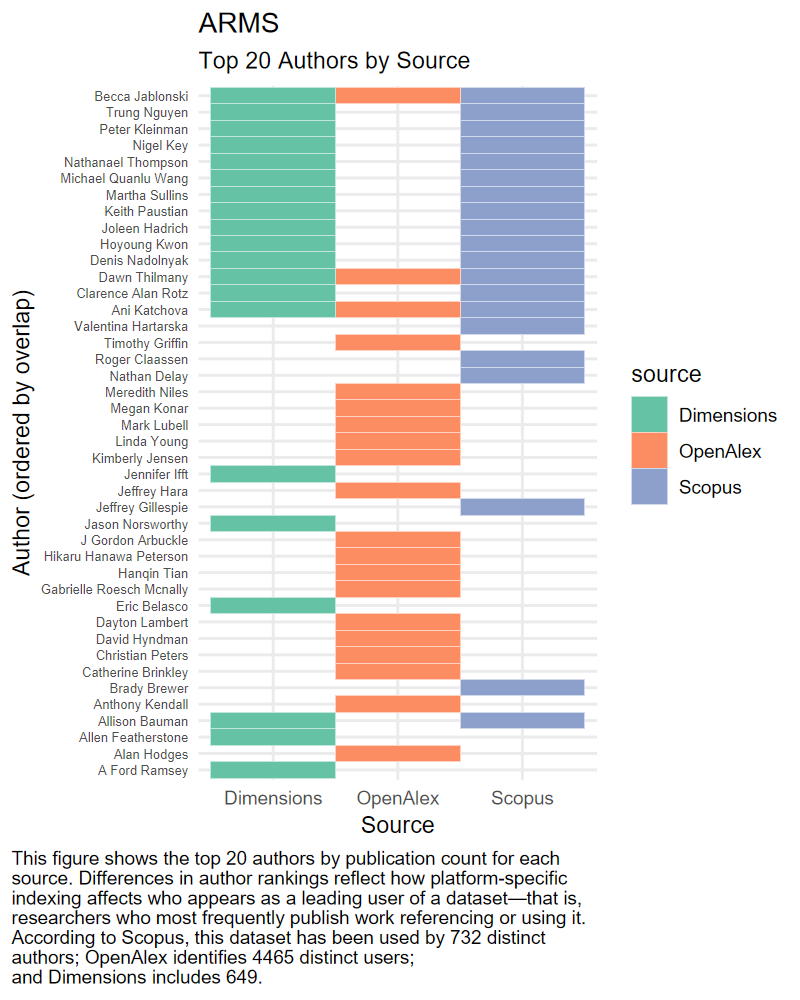
\includegraphics[keepaspectratio]{graphics/tilemaps/arms_top_20_author_overlap.png}}

\paragraph{Census of Ag}

The Census of Agriculture shows relatively higher agreement across
platforms, with many top authors appearing in multiple sources. However,
there are still noticeable differences, with some authors ranked highly
in one platform but not appearing at all in others. These discrepancies
are likely tied to variations in how author metadata and institutional
affiliations are recorded.

\pandocbounded{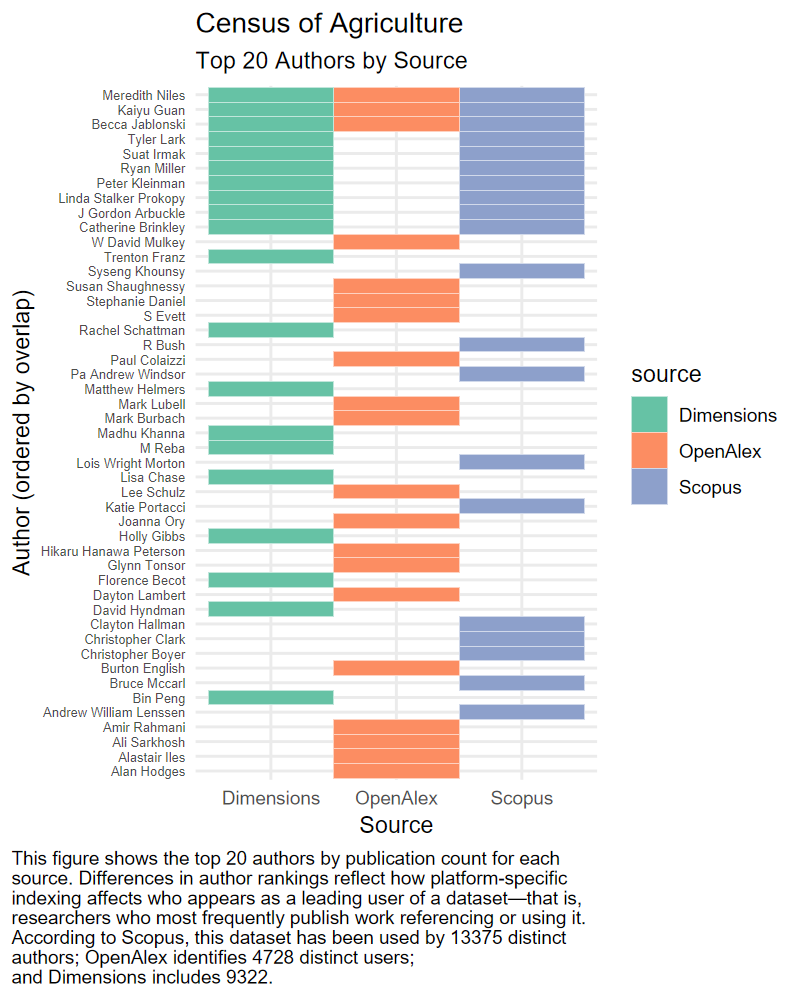
\includegraphics[keepaspectratio]{graphics/tilemaps/census_of_agriculture_top_20_author_overlap.png}}

\paragraph{FARA}

FARA displays substantial divergence in author coverage. A number of top
authors are visible in only one platform, and overlap across all three
is relatively limited. This dataset seems particularly affected by
platform-specific indexing practices---likely because much of the
associated research is interdisciplinary and published across a range of
journal types.

\pandocbounded{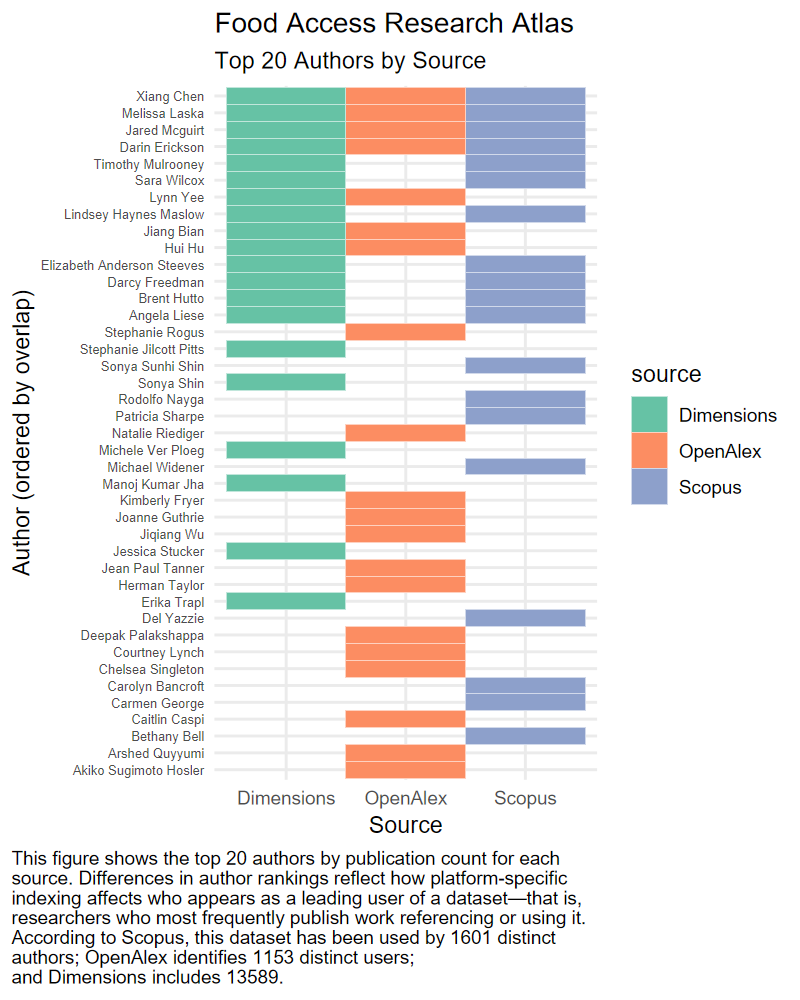
\includegraphics[keepaspectratio]{graphics/tilemaps/food_access_research_atlas_top_20_author_overlap.png}}

\paragraph{FoodAPS}

FoodAPS has uneven author coverage across platforms. While some authors
are picked up consistently, others are captured by only one source.
OpenAlex includes several authors who are not visible in Scopus or
Dimensions, suggesting that coverage differences may be especially
pronounced for newer researchers or those publishing in open-access
venues.

\pandocbounded{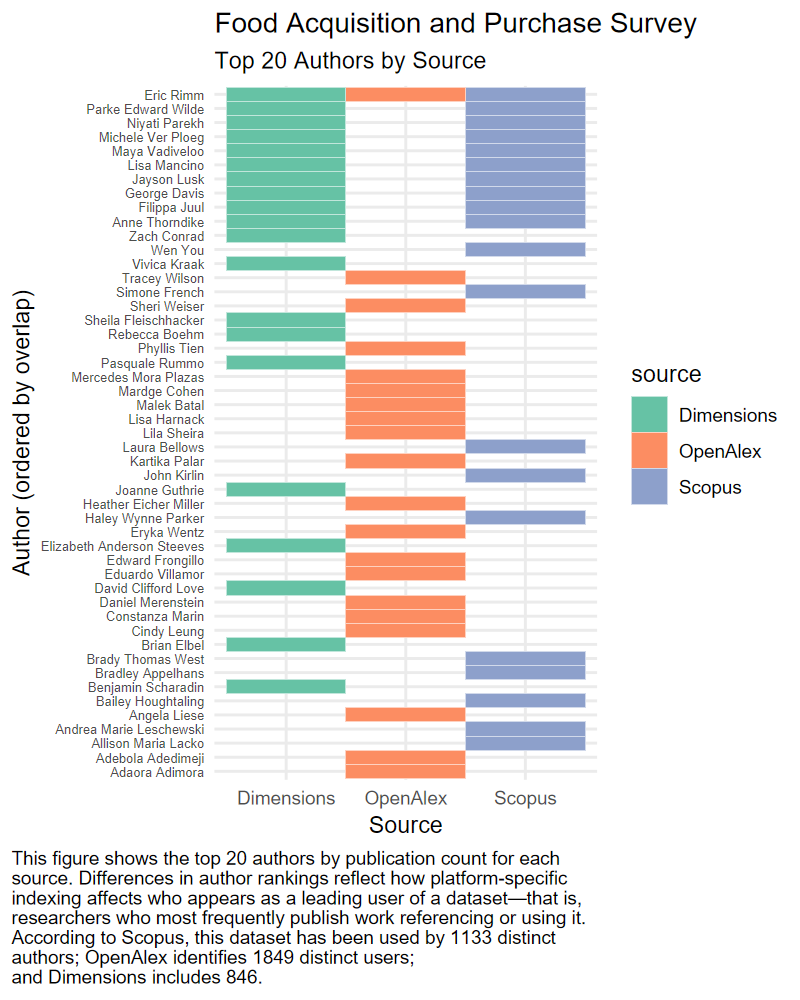
\includegraphics[keepaspectratio]{graphics/tilemaps/food_acquisition_and_purchase_survey_top_20_author_overlap.png}}

\paragraph{HFSSM}

The HFSSM dataset exhibits moderate agreement in author coverage. Most
top authors are represented in at least two sources, but each platform
still identifies several authors not seen in the others. This suggests
that while the dataset has relatively broad exposure, gaps remain that
could affect who is counted or highlighted in bibliometric analyses.

\pandocbounded{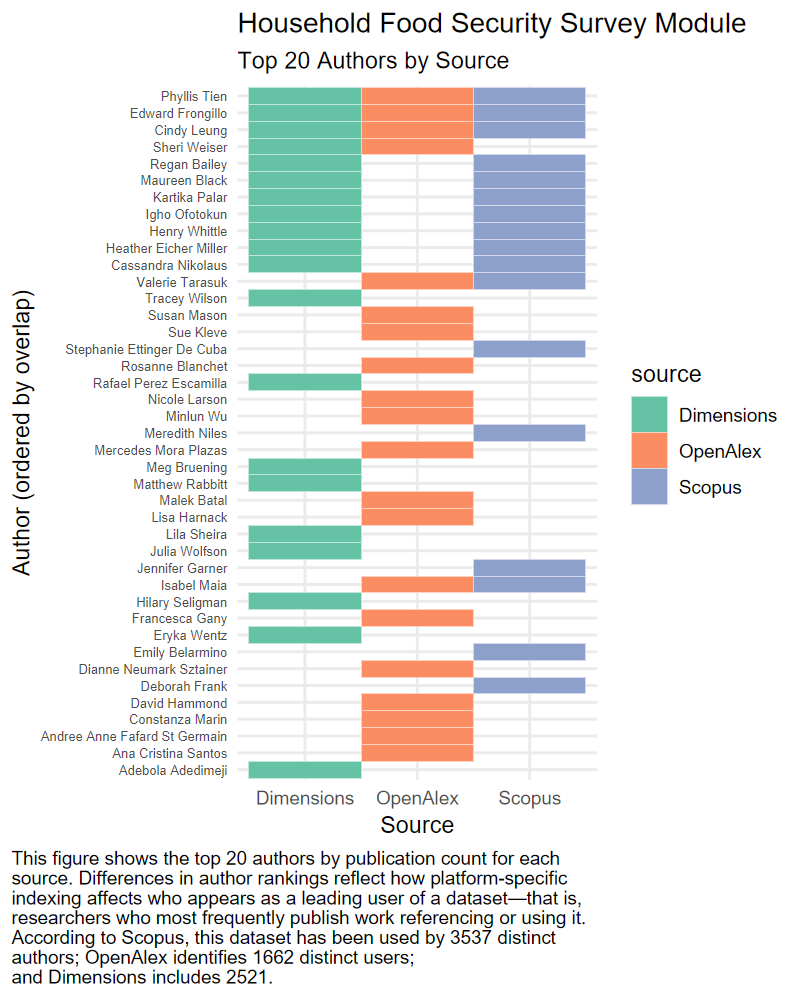
\includegraphics[keepaspectratio]{graphics/tilemaps/household_food_security_survey_module_top_20_author_overlap.png}}

\paragraph{RUCC}

RUCC shows the widest variation in author rankings. Many authors appear
in only one of the three sources, and very few are consistently
represented across all. This fragmentation likely reflects the broad
disciplinary scope of RUCC-related research, which spans public health,
demography, and social science---fields that are not uniformly indexed
across platforms.

\pandocbounded{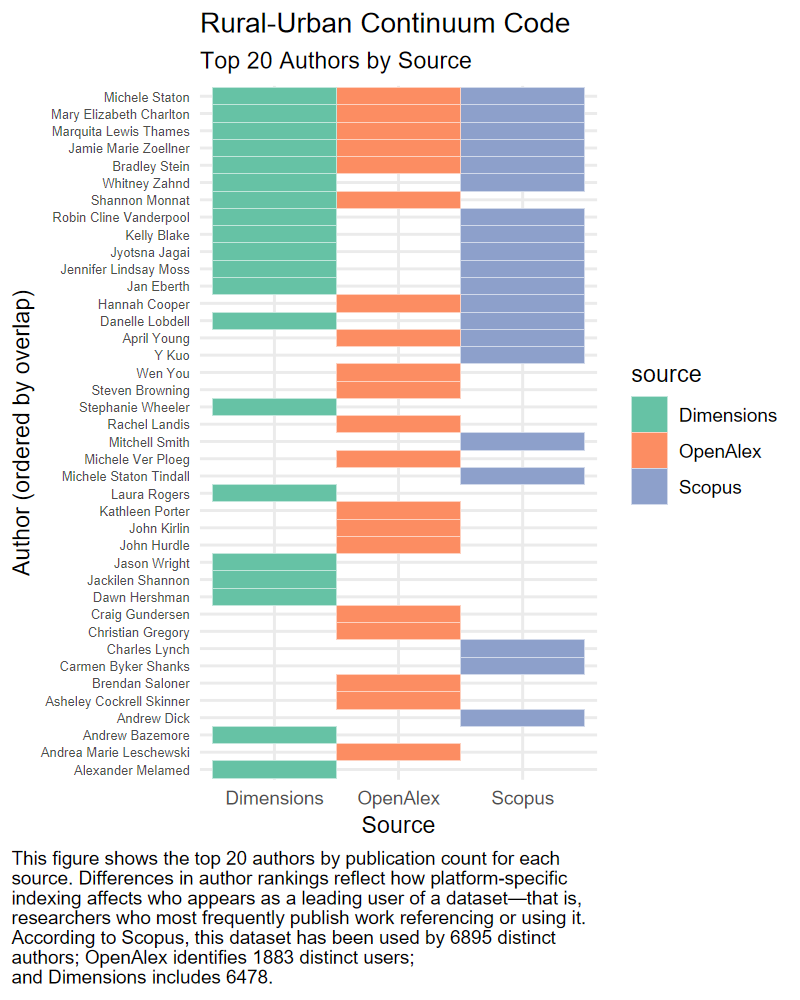
\includegraphics[keepaspectratio]{graphics/tilemaps/rural_urban_continuum_code_top_20_author_overlap.png}}

\subsubsection{Institutional Comparison}\label{institutional-comparison}

In addition to examining dataset mention coverage, the report also
evaluates differences in institutional representation across Scopus,
OpenAlex, and Dimensions. Each of the featured citation databases
represent some portion of the global research landscape, yet their
inclusion criteria and institutional coverage may vary. The purpose of
this analysis is to assess which institutions are represented in each
source.

\paragraph{Scopus}

\pandocbounded{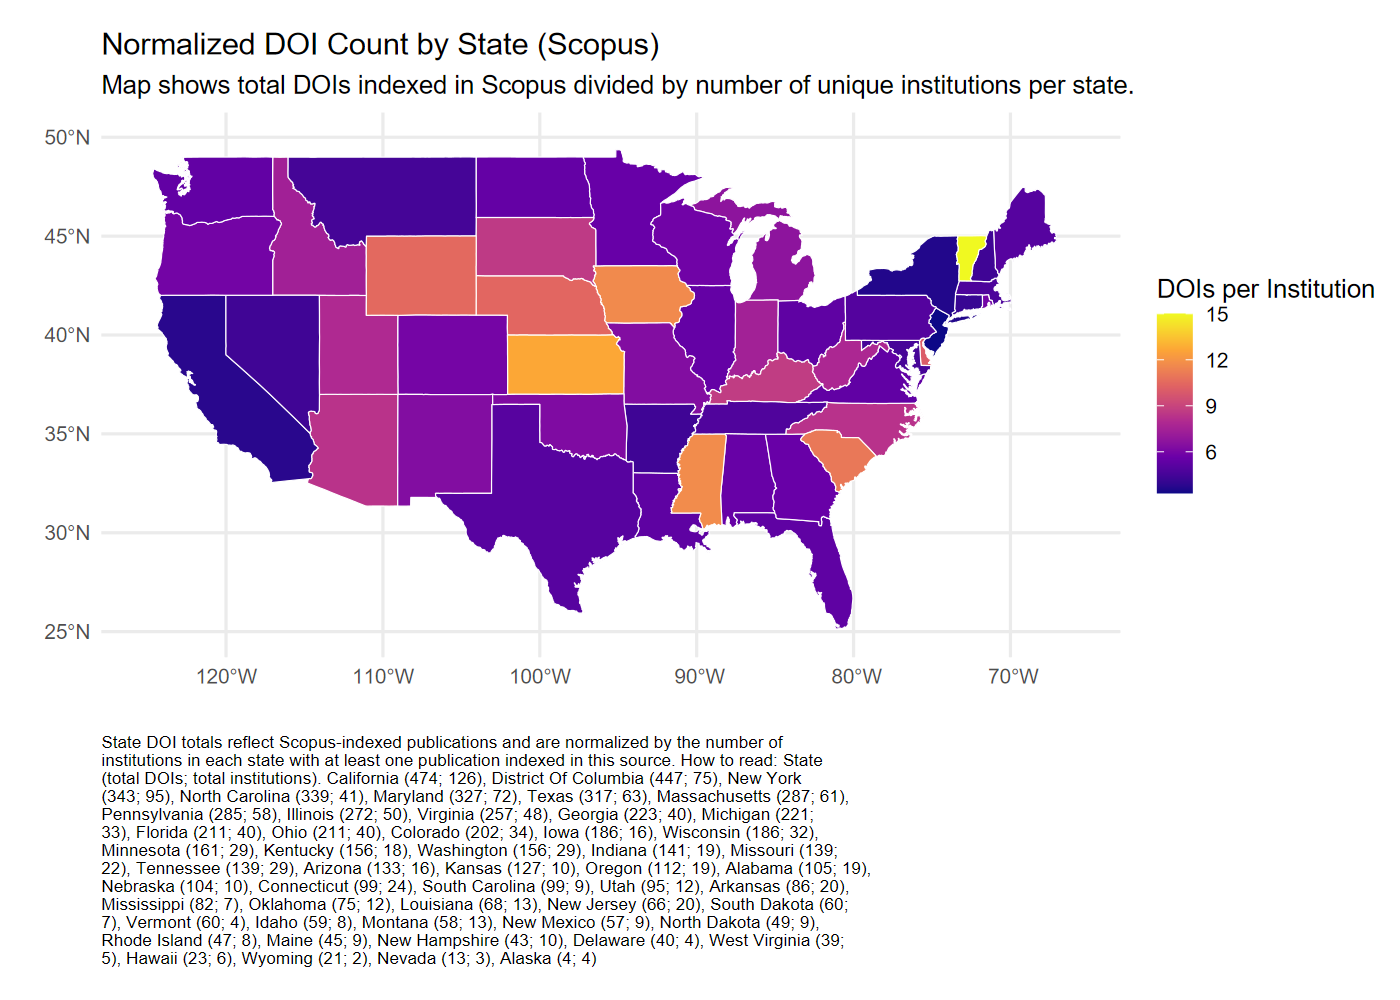
\includegraphics[keepaspectratio]{graphics/maps/scopus_normalized_dois_per_institution.png}}

\paragraph{Dimensions}

\pandocbounded{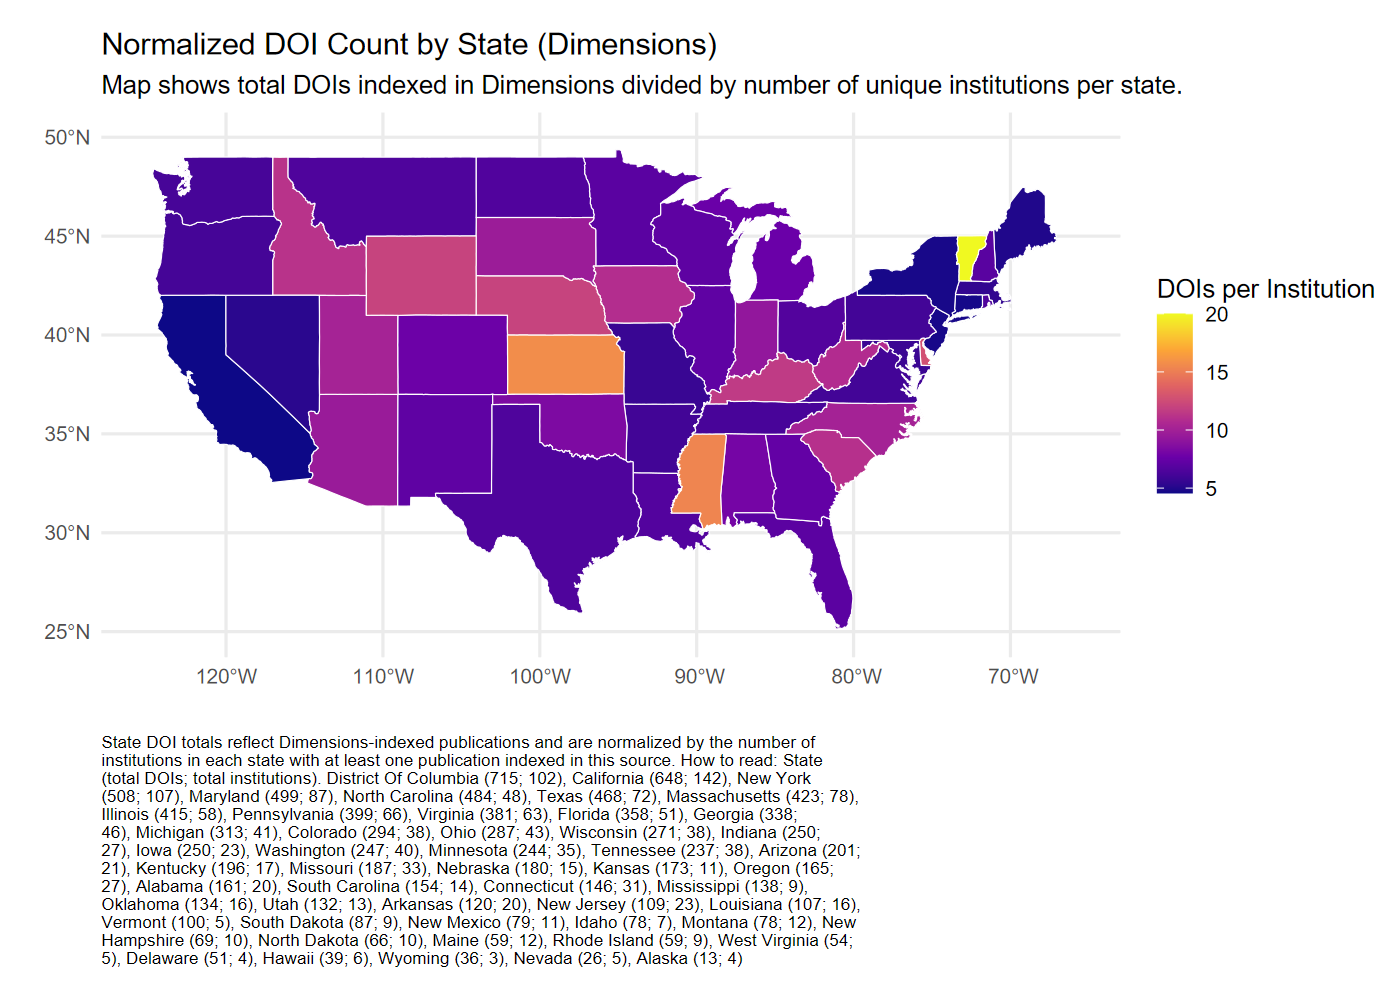
\includegraphics[keepaspectratio]{graphics/maps/dimensions_normalized_dois_per_institution.png}}

\paragraph{OpenAlex}

\pandocbounded{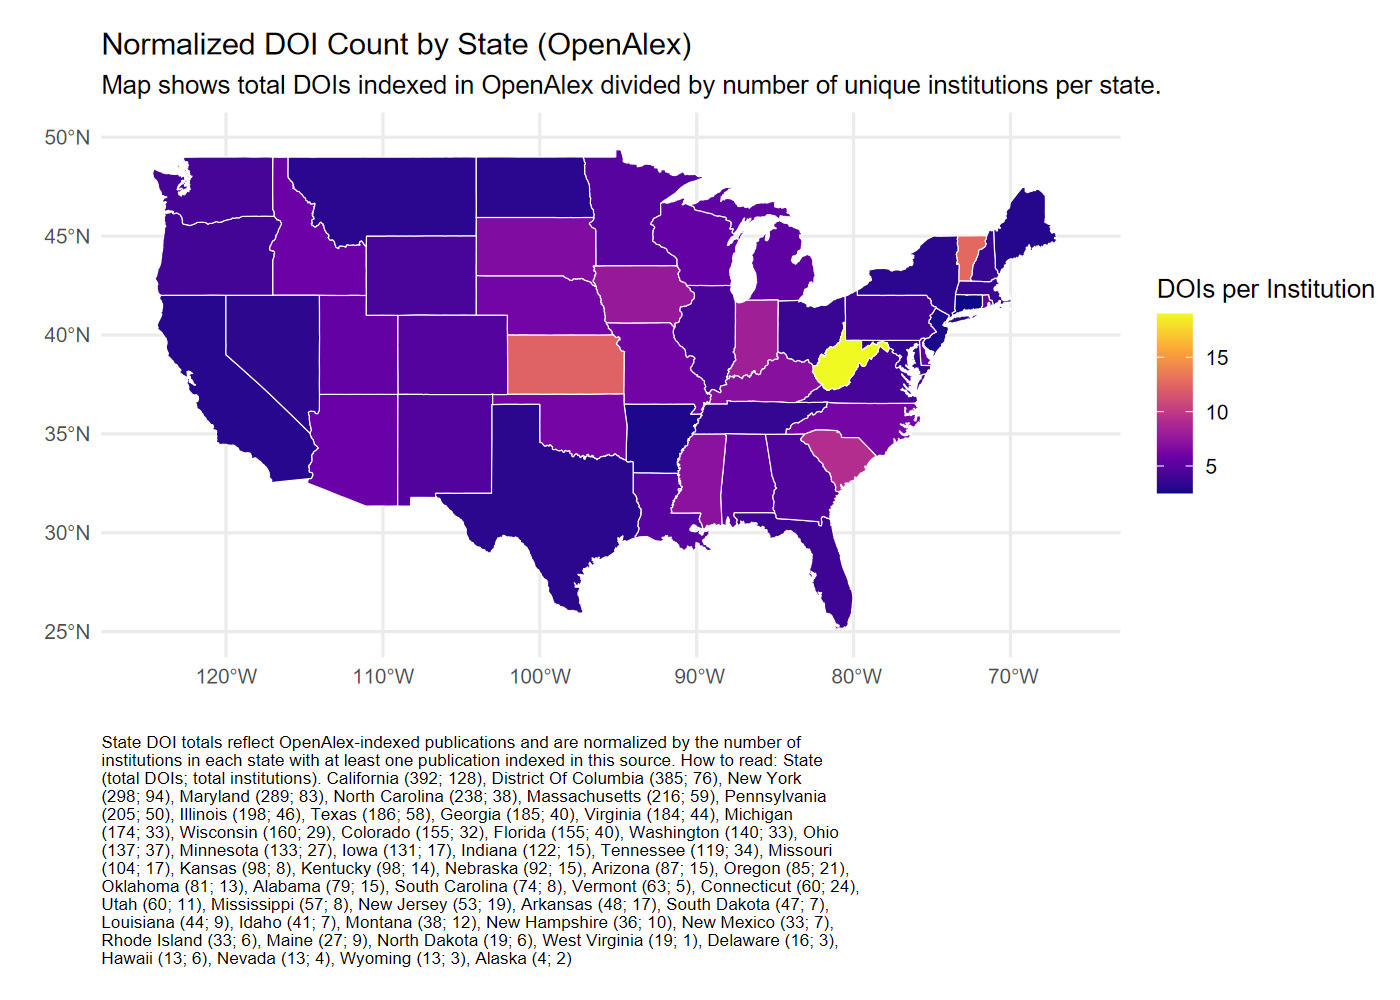
\includegraphics[keepaspectratio]{graphics/maps/openalex_normalized_dois_per_institution.png}}

\subsection{Conclusion}\label{conclusion}

This report compares how publications referencing the Census of
Agriculture are captured across Scopus, OpenAlex, and Dimensions. While
each platform provides partial visibility into dataset usage, the
overlap in coverage remains limited. Differences in indexing, topic
classification, and full-text availability lead to variation in which
publications, topics, and authors are discoverable. These findings
highlight how the choice of citation platform can shape perceptions of
research influence and dataset reach.

\newpage

\section*{Tables}\label{tables}
\addcontentsline{toc}{section}{Tables}

\begin{longtable}[]{@{}
  >{\raggedright\arraybackslash}p{(\linewidth - 6\tabcolsep) * \real{0.0877}}
  >{\raggedright\arraybackslash}p{(\linewidth - 6\tabcolsep) * \real{0.5702}}
  >{\raggedright\arraybackslash}p{(\linewidth - 6\tabcolsep) * \real{0.1491}}
  >{\raggedright\arraybackslash}p{(\linewidth - 6\tabcolsep) * \real{0.1930}}@{}}
\caption{Top 25 Topics by First Run
Count}\label{tbl-top25topics}\tabularnewline
\toprule\noalign{}
\begin{minipage}[b]{\linewidth}\raggedright
Topic ID
\end{minipage} & \begin{minipage}[b]{\linewidth}\raggedright
Topic Name
\end{minipage} & \begin{minipage}[b]{\linewidth}\raggedright
Full-Text Search Count
\end{minipage} & \begin{minipage}[b]{\linewidth}\raggedright
Total Count
\end{minipage} \\
\midrule\noalign{}
\endfirsthead
\toprule\noalign{}
\begin{minipage}[b]{\linewidth}\raggedright
Topic ID
\end{minipage} & \begin{minipage}[b]{\linewidth}\raggedright
Topic Name
\end{minipage} & \begin{minipage}[b]{\linewidth}\raggedright
Full-Text Search Count
\end{minipage} & \begin{minipage}[b]{\linewidth}\raggedright
Total Count
\end{minipage} \\
\midrule\noalign{}
\endhead
\bottomrule\noalign{}
\endlastfoot
T11610 & Impact of Food Insecurity on Health Outcomes & 549 & 78661 \\
T10010 & Global Trends in Obesity and Overweight Research & 272 &
111686 \\
T11066 & Comparative Analysis of Organic Agricultural Practices & 247 &
41275 \\
T12253 & Urban Agriculture and Community Development & 222 & 27383 \\
T10367 & Agricultural Innovation and Livelihood Diversification & 186 &
49818 \\
T11464 & Impact of Homelessness on Health and Well-being & 175 &
101019 \\
T12033 & European Agricultural Policy and Reform & 137 & 88980 \\
T10841 & Discrete Choice Models in Economics and Health Care & 126 &
66757 \\
T10596 & Maternal and Child Nutrition in Developing Countries & 116 &
118727 \\
T11898 & Impacts of Food Prices on Consumption and Poverty & 113 &
29110 \\
T11259 & Sustainable Diets and Environmental Impact & 109 & 45082 \\
T11311 & Soil and Water Nutrient Dynamics & 84 & 52847 \\
T10235 & Impact of Social Factors on Health Outcomes & 81 & 86076 \\
T10439 & Adaptation to Climate Change in Agriculture & 77 & 27311 \\
T11886 & Risk Management and Vulnerability in Agriculture & 73 &
44755 \\
T10226 & Global Analysis of Ecosystem Services and Land Use & 71 &
84104 \\
T10866 & Role of Mediterranean Diet in Health Outcomes & 70 & 76894 \\
T10969 & Optimal Operation of Water Resources Systems & 70 & 97570 \\
T10330 & Hydrological Modeling and Water Resource Management & 69 &
132216 \\
T11753 & Forest Management and Policy & 60 & 75196 \\
T12098 & Rural development and sustainability & 54 & 62114 \\
T10111 & Remote Sensing in Vegetation Monitoring and Phenology & 52 &
56452 \\
T10556 & Global Cancer Incidence and Mortality Patterns & 49 & 64063 \\
T11711 & Impacts of COVID-19 on Global Economy and Markets & 49 &
69059 \\
T12724 & Integrated Management of Water, Energy, and Food Resources & 47
& 40148 \\
\end{longtable}

\newpage

\begin{longtable}[]{@{}
  >{\raggedright\arraybackslash}p{(\linewidth - 6\tabcolsep) * \real{0.1154}}
  >{\raggedright\arraybackslash}p{(\linewidth - 6\tabcolsep) * \real{0.5846}}
  >{\raggedright\arraybackslash}p{(\linewidth - 6\tabcolsep) * \real{0.1308}}
  >{\raggedright\arraybackslash}p{(\linewidth - 6\tabcolsep) * \real{0.1692}}@{}}
\caption{Top 25 Journals by First Run
Count}\label{tbl-top25journals}\tabularnewline
\toprule\noalign{}
\begin{minipage}[b]{\linewidth}\raggedright
Journal ID
\end{minipage} & \begin{minipage}[b]{\linewidth}\raggedright
Journal Name
\end{minipage} & \begin{minipage}[b]{\linewidth}\raggedright
Full-Text Search Count
\end{minipage} & \begin{minipage}[b]{\linewidth}\raggedright
Total Count
\end{minipage} \\
\midrule\noalign{}
\endfirsthead
\toprule\noalign{}
\begin{minipage}[b]{\linewidth}\raggedright
Journal ID
\end{minipage} & \begin{minipage}[b]{\linewidth}\raggedright
Journal Name
\end{minipage} & \begin{minipage}[b]{\linewidth}\raggedright
Full-Text Search Count
\end{minipage} & \begin{minipage}[b]{\linewidth}\raggedright
Total Count
\end{minipage} \\
\midrule\noalign{}
\endhead
\bottomrule\noalign{}
\endlastfoot
S2764628096 & Journal of Agriculture Food Systems and Community
Development & 57 & 825 \\
S115427279 & Public Health Nutrition & 51 & 3282 \\
S206696595 & Journal of Nutrition Education and Behavior & 41 & 3509 \\
S15239247 & International Journal of Environmental Research and Public
Health & 39 & 59130 \\
S4210201861 & Applied Economic Perspectives and Policy & 39 & 647 \\
S10134376 & Sustainability & 35 & 87533 \\
S5832799 & Journal of Soil and Water Conservation & 34 & 556 \\
S2739393555 & Journal of Agricultural and Applied Economics & 34 &
329 \\
S202381698 & PLoS ONE & 30 & 143568 \\
S124372222 & Renewable Agriculture and Food Systems & 30 & 426 \\
S200437886 & BMC Public Health & 28 & 18120 \\
S91754907 & American Journal of Agricultural Economics & 28 & 876 \\
S18733340 & Journal of the Academy of Nutrition and Dietetics & 27 &
5301 \\
S78512408 & Agriculture and Human Values & 27 & 938 \\
S110785341 & Nutrients & 25 & 30911 \\
S2764593300 & Agricultural and Resource Economics Review & 25 & 247 \\
S4210212157 & Frontiers in Sustainable Food Systems & 23 & 3776 \\
S63571384 & Food Policy & 20 & 1069 \\
S69340840 & The Journal of Rural Health & 20 & 749 \\
S4210234824 & EDIS & 18 & 3714 \\
S19383905 & Agricultural Finance Review & 18 & 327 \\
S119228529 & Journal of Hunger \& Environmental Nutrition & 17 & 467 \\
S43295729 & Remote Sensing & 14 & 33899 \\
S2738397068 & Land & 14 & 9774 \\
S80485027 & Land Use Policy & 14 & 4559 \\
\end{longtable}

\newpage

\begin{longtable}[]{@{}
  >{\raggedright\arraybackslash}p{(\linewidth - 6\tabcolsep) * \real{0.1818}}
  >{\raggedright\arraybackslash}p{(\linewidth - 6\tabcolsep) * \real{0.3117}}
  >{\raggedright\arraybackslash}p{(\linewidth - 6\tabcolsep) * \real{0.2208}}
  >{\raggedright\arraybackslash}p{(\linewidth - 6\tabcolsep) * \real{0.2857}}@{}}
\caption{Top 25 Authors by First Run Count
Table}\label{tbl-top25authors}\tabularnewline
\toprule\noalign{}
\begin{minipage}[b]{\linewidth}\raggedright
Author ID
\end{minipage} & \begin{minipage}[b]{\linewidth}\raggedright
Author Name
\end{minipage} & \begin{minipage}[b]{\linewidth}\raggedright
Full-Text Search Count
\end{minipage} & \begin{minipage}[b]{\linewidth}\raggedright
Total Count
\end{minipage} \\
\midrule\noalign{}
\endfirsthead
\toprule\noalign{}
\begin{minipage}[b]{\linewidth}\raggedright
Author ID
\end{minipage} & \begin{minipage}[b]{\linewidth}\raggedright
Author Name
\end{minipage} & \begin{minipage}[b]{\linewidth}\raggedright
Full-Text Search Count
\end{minipage} & \begin{minipage}[b]{\linewidth}\raggedright
Total Count
\end{minipage} \\
\midrule\noalign{}
\endhead
\bottomrule\noalign{}
\endlastfoot
A5016803484 & Heather A. Eicher‐Miller & 15 & 140 \\
A5024975191 & Edward A. Frongillo & 13 & 351 \\
A5055158106 & Becca B.R. Jablonski & 12 & 60 \\
A5047780964 & Meredith T. Niles & 11 & 200 \\
A5076121862 & Sheri D. Weiser & 10 & 241 \\
A5068812455 & Cindy W. Leung & 10 & 170 \\
A5062679478 & J. Gordon Arbuckle & 10 & 68 \\
A5015017711 & Jeffrey K. O'Hara & 10 & 27 \\
A5081656928 & Whitney E. Zahnd & 9 & 147 \\
A5002438645 & Phyllis C. Tien & 8 & 244 \\
A5035584432 & Angela D. Liese & 8 & 172 \\
A5027684365 & Dayton M. Lambert & 8 & 110 \\
A5081012770 & Linda J. Young & 8 & 51 \\
A5008463933 & Catherine Brinkley & 8 & 34 \\
A5030548116 & Michele Ver Ploeg & 8 & 33 \\
A5056021318 & Nathan Hendricks & 7 & 320 \\
A5024248662 & Adebola Adedimeji & 7 & 137 \\
A5002732604 & Julia A. Wolfson & 7 & 137 \\
A5038610136 & Christopher N. Boyer & 7 & 115 \\
A5044317355 & Daniel Merenstein & 7 & 113 \\
A5006129622 & Carmen Byker Shanks & 7 & 103 \\
A5060802257 & Tracey E. Wilson & 7 & 102 \\
A5050792105 & Jennifer L. Moss & 7 & 90 \\
A5032940306 & Lisa Harnack & 7 & 89 \\
A5024127854 & Eduardo Villamor & 7 & 84 \\
\end{longtable}




\end{document}
